\documentclass[a4paper,12pt]{article}
\usepackage[utf8]{inputenc}
\usepackage[english]{babel}
 \usepackage[usenames,dvipsnames]{xcolor}
 \usepackage{amssymb}
\usepackage{amsmath,mathrsfs}
\usepackage{amsfonts}
 \usepackage[all]{xy}

 \usepackage{graphicx}
 \usepackage{enumerate}
 \usepackage{wrapfig}
\usepackage{amsthm}
\usepackage{authblk}

\usepackage{hyperref}
\hypersetup{
    colorlinks=true,       % false: boxed links; true: colored links
    linkcolor=red,          % color of internal links (change box color with linkbordercolor)
    citecolor=black,        % color of links to bibliography
    filecolor=cyan,         % color of file links
    urlcolor=magenta        % color of external links
}
 \usepackage[usenames,dvipsnames]{xcolor}
 \usepackage{mathbbol}
\usepackage{pgf,tikz}
\usetikzlibrary{calc}

 \def\ZZ{\mathbb{Z}}
 \def\NN{\mathbb N}
 \def\r{\mathfrak{r}}
 \def\D{\mathcal{D}}
 \def\Z{\mathbb{Z}}
 \def\H{\mathbb{H}}
 \def\M{\mathcal{M}}
 \def\s{\mathfrak S}
 \def\v{\mathfrak v}
 \def\chleq{\leq\!\!\!\leq }
 \def \chll{<\!\!\!<}

 \def\stab{\mathrm{Stab}}
\def\Kbar{\overline{K}}
\def\au{\overrightarrow{u}}
 \def\U{\mathcal U}
 \def\ab{ \mathrm{ab}}
 \def\Hom{\mathrm{Hom}}
 \def\GGL{\SO_0(1,2)}
 \def\isom{Isom}
 \def\lsem{[\![}
 \def\rsem{]\!]}
\def\V{\mathcal V}
\def\A{\mathcal A}
\def\TT{\mathcal T}
\def\R{\mathbb{R}}
\def\E{\mathbf E}
\def\G{\mathbf G}
\def\S{\mathcal S}
\def\calC{\mathcal C}
\def\adm{\P}

\def\T{\mathcal{T}}
\def\rot{\mathbf{rot}}
\def\div{\mathbf{div}}
\def\grad{\overrightarrow{\mathbf{grad}}}
\def\d{\mathrm{d}}
\def\S{\mathcal{S}}
\def\K{\mathbf K}
\def\D{\mathcal{D}}
\def\SO{\mathrm{SO}}
\def\E{\mathbb{E}}
\def\BTZ{{\E_{0}^{1,2}}}
\def\sing{\mathrm{Sing}}
\def\RR{\mathbb{R}}
\newcommand{\mass}[1]{{\mathbb E}^{1,2}_{#1}}
\def\isom{\mathrm{Isom}}
\def\L{\mathrm{L}}
\def\graph{\mathrm{Graph}}
\def\Teich{\mathrm{Teich}}
\def\Hol{\mathrm{Hol}}
\def\Reg{\mathrm{Reg}}
\def\fix{\mathrm{Fix}}
\def\teich{\mathrm{Teich}}
\def\susp{\mathrm{susp}}
\def\BTZext{\mathrm{Ext}_{BTZ}}
\def\pgcd{M_1\wedge M_2}
\def\ppcm{M_1\vee M_2}
\def\reg{\Reg}
\def\CC{\mathcal{C}}
\def\DD{\mathbb{D}}
\def\V{\mathcal V}
\def\F{\mathcal F}
\def\T{\mathcal{T}}
\def\G{\mathbf G}
\def\S{\mathcal S}
\def\W{\mathcal W} 
\def\MM{\overline M}
\def\SO{\mathrm{SO}}
\def\stab{\mathrm{Stab}}
\def\R{\mathcal R}
\def\CC{\mathbb{C}}
\def\J{\mathcal{J}}
\def\SS{\mathbb{S}}
\def\quadform{\mathbf{g}}
\def\Cell{\mathcal C}
\def\Cone{\mathcal D}
\def\Future{\mathcal F}
\def\E{\mathbb{E}}
\def\sing{\mathrm{Sing}}
\def\isom{\mathrm{Isom}}
\def\d{\mathrm{d}}
\def\Z{\mathbb Z}
\def\N{\mathbb{N}}
\def\reg{\mathrm{Reg}}
\def\D{\mathcal{D}}
\def\BTZ{\mathbb{E}^{1,2}_0}
\def\U{\mathcal{U}}
\def\fix{\mathrm{Fix}}
\def\BTZext{\mathrm{Ext}_{\mathrm{BTZ}}}
\def\Reg{\mathrm{Reg}}
\def\mink{\mathbb{E}^{1,2}}
\def\Dbar{\overline{\D}}
\def\adm{\mathcal{P}}
\def\EH{\mathcal{H}}
\def\grad{\mathrm{grad}}
\def\Hol{\mathrm{Hol}}
\def\Cat{\mathbf{C}}
\def\Top{\mathbf{Top}}
\def\M{\mathcal M}
\def\cotan{\mathrm{ct}}
\def\catGX{\mathbf{Var_{G,X}}}
\newcommand{\catE}[1]{\mathbf{Var_{\mass{#1}}}}
\newcommand{\catX}[1]{\mathbf{Var_{X_{#1}}}}
\def\Im{\mathrm{Im}}
\def\et{~\text{et}~}
\def\DD{\mathbb{D}}
\def\r{\mathfrak{r}}
\def\massA{\mass{\geq 0}}
\def\pgcd{M_1 \wedge M_2}
\def\ppcm{M_1 \vee M_2}
\def\teich{\mathrm{Teich}}
\def\fix{\mathrm{Fix}}
\def\dec{\mathrm{dec}}
\def\sing{\mathrm{Sing}}
\def\Hol{\mathrm{Hol}}
\def\so{\mathfrak{so}}
\def\pen{\mathcal{P}}
\def\susp{\mathrm{susp}}
\def\UU{\mathbb{U}}
\def\PP{\mathbb{P}}
\def\P{\mathcal{P}}
\def\Hom{\mathrm{Hom}}
\def\a{\lambda}
\def\b{\mu}
\def\cc{\beta}
\def\CellPSigmabar{\overline{\P}_\TT}
\def\dd{\alpha}
\def\A{\mathcal A}
\def\B{\mathcal B}
\def\CellPSigma{\P_\TT}
\def\GG{\isom_0(\mass{})}
\def\Hbar{\overline{\H^2}}
\def\RP{\mathbb{RP}^1}
\def\PSL{\mathrm{PSL}}
\def\HS{\mathbb{HS}}
\def\struc{\mathbf{Struct}}
\def\GL{\mathrm{GL}}
\def\SL{\mathrm{SL}}
\def\G{\mathcal G}
\def\Aut{\mathrm{Aut}}
\def\supp{\mathrm{supp}}
\def\Homeo{\mathrm{Homeo}}
\def\cool{{cool}}
\def\ord{\mathrm{Ord}}
\def\vecM{\overrightarrow{\E}^{1,2}}
\def\X{\overrightarrow X}
\def\gradH{{\overrightarrow{\grad} \mathcal{H}_{\bar\kappa}}}
\def\calP{\mathcal{P}}
\newcommand{\function}[5]{\displaystyle#1:\begin{array}{l|rcl}
& \displaystyle #2 & \longrightarrow & \displaystyle #3 \\
	& \displaystyle #4 & \longmapsto & \displaystyle #5 \end{array}}
\newcommand{\functiondeux}[7]{\displaystyle#1:\begin{array}{l|rcl}
& \displaystyle #2 & \longrightarrow & \displaystyle #3 \\
	& \displaystyle #4 & \longmapsto & \displaystyle #5 \\ 
	& \displaystyle #6 & \longmapsto & \displaystyle #7\end{array}}	
\newcommand{\functiontrois}[9]{\displaystyle#1:\begin{array}{l|rcl}
& \displaystyle #2 & \longrightarrow & \displaystyle #3 \\
	& \displaystyle #4 & \longmapsto & \displaystyle #5\\
	& \displaystyle #6 & \longmapsto & \displaystyle #7\\
	& \displaystyle #8 & \longmapsto & \displaystyle #9\end{array}}	
\newcommand{\functionn}[4]{\displaystyle\begin{array}{l|rcl}
& \displaystyle #1 & \longrightarrow & \displaystyle #2 \\
	& \displaystyle #3 & \longmapsto & \displaystyle #4 \end{array}}


\definecolor{MyGreen}{rgb}{0.0,.5,0.0}
\newcommand{\edl}[1]{{\color{MyGreen}{#1}}}
\newcommand{\leo}[1]{{\color{MyGreen} [\textbf{Leo: } #1]}}
\newcommand{\tautilde}[2]{\widetilde\tau_{#1,#2}}
\definecolor{MyDarkRed}{rgb}{0.7,0,0}
\newcommand{\edt}[1]{{\color{MyDarkRed}{#1}}}
\usepackage{float}
%%% Start of metadata


\title{Alexandrov Theorem for 2+1 flat radiant spacetimes}
\author{L\'eo Brunswic}
\affil{Huawei Shanghai Postdoctoral Research Center and  JiaoTong University Shanghai, Shanghai, China}
% First author

% \givenname{Léo}
% \surname{Brunswic}
% \address{Huawei Shanghai Postdoctoral Research Center, E2F2 }
% \email{math@brunswic.fr}
% \urladdr{leo.brunswic.fr}

% Second author (uncomment if necessary)
%
%\author{}
%\givenname{}
%\surname{}
%\address{}
%\email{}
%\urladdr{}
%
% (Add a similar block for other authors)
%
% Title and author both have running head options:
%
% \title[Running head title]{Main title}
% \author[Running head author]{Author}

%
% give a separate \keyword and \subject line for each keyword/phrase or 
% subject class e.g.\ \keyword{framed link} \subject{primary}{msc2010}{57M25}

% \keyword{}
% \subject{primary}{msc2010}{}
% \subject{secondary}{msc2010}{}

% Fill in the reference number if your article is stored on the arXiv
% e.g.\ \arxivreference{math.GT/0512347} or \arxivreference{1203.4984}.
% The newer style reference numbers (with a period) do not require the
% prefix arxiv: or math.NT/ or anything else. Just the reference
% number is sufficient.
% 
% \arxivreference{}

%%% End of metadata

%%% Start of user-defined macros %%%
%
% Theorem-type environments. There are two predefined styles:
%
% \theoremstyle{plain}: for theorems, corollaries etc with heading 
% bold and left justified, optional note bracketed in roman type
% and statement in slanted type. This is the default style.
%
% \theoremstyle{definition}: (alias remark) for definitions, remarks 
% etc with heading bold and left justified, optional note as before but
% with statement in roman type.
% 
% Some sample \newtheorem's (delete these unless you need
% them and insert your own):
%

\newtheorem{theo}{Theorem}	% Standard theorem environment

\newtheorem{lem}{Lemma}[section]		 % Lemma environment with numbering 
\newtheorem{prop}[lem]{Proposition}
\newtheorem{defiprop}[lem]{Definition-Proposition}
\newtheorem{cor}[lem]{Corollary}
\newtheorem{example}[lem]{Example}
\newtheorem*{theon}{Theorem}
\newtheorem*{problem}{Problem}
\newenvironment{claim}[1]{\par\noindent\underline{Claim:}\space#1}{}
\newenvironment{claimproof}[1]{\par\noindent\underline{Proof:}\space#1}{\hfill $\blacksquare$}

%									 % consecutive to theorems
\newtheorem*{zlem}{Zorn's Lemma}	 % A special unnumbered lemma.
%
\theoremstyle{definition}
\newtheorem{defi}[lem]{Definition}	% Definition environment with 
%									 % numbering consecutive to theorems
\newtheorem*{rem}{Remark}			 % Unnumbered environment for remarks.
%
% Type your macros (\newcommand's etc) below.
%

\def\CatSpread{\mathbf{Spr}}
\def\CatSingGX{\mathbf{SingGX}}

%%% End of user-defined macros %%%

\begin{document}

\maketitle
\begin{abstract}
Let $\Sigma$ be a closed surfaces endowed with a locally Euclidean metric with conical singularities $(\theta_i)_{i\in \lsem1,s\rsem}$.
Asuming all the $\theta_i$ are bigger than $2\pi$, Fillastre showed that one can realize the universal covering of $\Sigma$  as the boundary of a convex Fuchsian polyhedra in 3-dimensional Minkowski space $\mass{}$ in a unique manner up to the action of $ \SO(1,2)\ltimes \RR^3$ the affine isometry group of Minkowski space. 
The proof employed a so-called deformation method which is non-constructive.
We adapt a variationnal method previously used by Volkov, Bobenko, Izmestiev and Fillastre on similar problems to provide an effective proof of Fillastre Theorem.
In passing, we extend Fillastre's Theorem as follows. Without assumptions on the $\theta_i$ and for any choice of non-negative $(\kappa_i)_{i\in \lsem1,s\rsem}$ such that $\kappa_i<\theta_i$ and $\kappa_i\leq 2\pi$, there exists a unique couple $(M,P)$ where $M$ belongs to a class of singular locally Minkowski manifolds we define with $s$ singular lines of respective conical angle $\kappa_i$; and $P$ is convex polyhedron in $M$ whose boundary $\partial P$ is Cauchy-surface isometric to $\Sigma$, the $i$-th conical singularity of $\partial P$ lying on the $i$-th singular line of $M$. Fillastre Theorem is the special case $\kappa_i=2\pi$ and we note that some Penner-Epstein convex hull constructions correspond to the special case $\kappa_i=0$. 

\end{abstract}
%%%%%%%%%%%%%%%%%%%% Start of main body of article
\tableofcontents

\section{Introduction}
\subsection{Alexandrov Theorem} \

	
		Let $C$ be a cube in the 3-dimensional Euclidean space $\E^3$
		and consider $\Sigma:=\partial C$
		its boundary represented on the figure. On the one hand, $\Sigma$ is a surface homeomorphic to the 2-dimensional sphere $\SS^2$; on the other hand, $\Sigma$ is naturally endowed with a locally Euclidean metric with 6 conical singularities each of angle $3\pi/2$. \\
		\begin{wrapfigure}{r}{0.5\textwidth}
			\includegraphics[width=0.45\linewidth]{cube.png}
			\includegraphics[width=0.45\linewidth]{patron_cube.png}
		\end{wrapfigure}
		More generally, the boundary of any compact convex polyhedron in $\E^3$ is homeomorphic to the 2 dimensional sphere and is naturally endowed with a locally Euclidean metric with conical singularities of angles lesser than $2\pi$.
		
		A classical theorem of Alexandrov \cite{MR13540} shows that this construction is actually bijective.
		\begin{theon}[\cite{MR13540}]\label{theo:mr} Let $\Sigma$ be a locally Euclidean
			surface with conical singularities of angles lesser than $2\pi$ and homeomorphic to the sphere $\SS^2$,
			there exists a compact convex polyhedron $P$ in $\E^3$ such that $\partial P$ is isometric to $\Sigma$. Furthermore, two such polyhedra are congruent.
		\end{theon}
		Using a so-called deformation method, Alexandrov proved generalizations to convex polyhedron in $\H^3$ and $\SS^3$; this method is however not effective since it does not provide an efficient way to construct the convex polyhedra these Theorems predict.
\subsection{Generalizations to spaceforms and main result}
		
		In the 2000s,
		Izmestiev and Bobenko
		gave a new proof of Alexandrov theorem by a variational, therefore effective, method. See \cite{kane2009pseudopolynomial} for an complexity analysis of the resulting algorithm. Rivin, Hodgson, Schlenker and Fillastre
		proved generalizations to Lorentzian spaceforms (Minkowski, de Sitter and Anti-de Sitter) in which case conical singularities of the locally Euclidean surface have angles greater than $2\pi$.
		The Alexandrov problem can then be stated in a more general context that has been recently studied in a systematic way by Fillastre and Izmestiev. 
		
		\begin{problem}\label{rem:closed_surface_genus_endowed}
		
		
		
		 Let $\Sigma$ be a closed surface of genus $g$ endowed with singular metric of constant curvature
	 $K\in \{-1,0,1\}$ and cone angles all bigger that
	 $2\pi$ (case $\varepsilon=-)$ or all lesser than $2\pi$ (case $\varepsilon =+$).
		 Denoting by $X_K^\varepsilon$ the model space of constant curvature $K$ Riemannian if $\varepsilon=+$ and Lorentzian if $\varepsilon=-$.
        
         Is there a convex polyhedral Fuchsian realization of $\Sigma$  in $X_{K}^{\varepsilon}$.
		 Furthermore, is this polyhedron unique up to congruence?
		\end{problem}

    \begin{wrapfigure}{r}{0.4\textwidth}
		 \begin{tabular}{|c|c|c|c|c|}\hline
			$g$	&$K$	&$\varepsilon$	& DM & VM \\ \hline
			$0$	&$0$	&$+$&\cite{MR13540}&\cite{MR2410380} \\
			$0$	&$-1$	&$+$&\cite{MR2127379}& \\
			$0$	&$1$	&$+$&\cite{MR2127379}& \\
			$0$	&$1$	&$-$&\cite{Hodgson1993}& \\ \hline
			$1$	&$-1$	&$+$&&\cite{MR2469522}\\
			$1$	&$1$	&$-$&& \cite{MR2813423}\\
			\hline
			$\geq2$&$-1$&$+$&\cite{MR2313089}& \\
			$\geq2$&$-1$&$-$&\cite{MR2794916}& \\
			$\geq2$&$0$	&$-$&\cite{MR2794916}& [B] \\
			$\geq2$&$1$	&$-$&\cite{Schlenker2001hyperbolic}& \\ \hline
		 \end{tabular}
		\end{wrapfigure}
		The signature of the $X_K^{\varepsilon}$ and the Gauss-Bonnet formula impose  constraints on $(g,K,\varepsilon)$; the table on the right is based upon \cite{fillastre:hal-00535675} and sums up all possible situations
together with references to proofs by deformation (DM) and/or variational (VM) methods; [B] refers to the present work.
		
    
    Proving Fillastre Theorem --- case $(g,K,\varepsilon)=(\geq2,0,-)$ and $X_K^\varepsilon$ is Minkowski space $ \E^{1,2}$ --- by a variational method is the primary motivation of the present work. In this setting, ``convex polyhedral Fuchsian realization'' means that we build a triple $(\rho,\iota,P)$ where $\rho$ is a representation of $\pi_1(\Sigma)\rightarrow \mathrm{Isom}(\mass{})$, a $\rho$-equivariant embedding $\iota:\widetilde\Sigma\rightarrow \mass{}$ of the universal covering  of $\Sigma$ and a convex globally $\rho$-invariant polyhedron $P$; with the additionnal hypothesis that $\rho$ fixes a point and acts co-compactly the hyperboloid model of the hyperbolic plane $\H^2=\{(t,x,y)~|~t^2-x^2-y^2=1,t>0\}\subset \mass{}$  

	To this end, we adapt the variational method successfully used by Bobenko, Fillastre and Izmestiev \cite{MR2410380,MR2469522,MR2813423}; we derive Alexandrov-Fillastre, and obtain a generalization to a class of singular locally Minkowski 3-manifolds: radiant singular flat spacetimes we shall describe thereafter. 
	

	 \begin{theon}\label{theo:closed_locally_euclidean_surface} Let $\Sigma$ be a closed locally Euclidean surface of genus $g$ with $s$ marked conical singularities\footnote{We allow marked conical singularities with angle $2\pi$ hence not singular but marked nonetheless.}  of angles $(\theta_i)_{i\in \lsem 1,s\rsem}$.
For all $$\kappa\in \left(\prod_{i=1}^s[0,\min(\theta_i,2\pi)]\right) \setminus \{(\theta_i)_{i\in \lsem 1,s\rsem}\},$$ there exists a radiant singular flat spacetimes $M$ homeomorphic to $\Sigma\times \RR$ with exactly $s$ singular lines of angles $\kappa_1,\cdots,\kappa_s$ and
a convex polyhedron $P\subset M$ which boundary is isometric to $\Sigma$. The boundary of $P$ is a Cauchy-surface of $M$.
	
	Furthermore, if $\forall i\in\lsem 1,s\rsem,\kappa_i<\theta_i$ then $(M,P)$ is unique up to equivalence.
				
	Finally, if for some $i\in\lsem 1,s\rsem,\theta_i\leq \pi$ and $\kappa\in \RR_+^s$ is such that $\kappa_i>\theta_i$ then there is no such couple $(M,P)$.
	\end{theon}
	\begin{rem}\label{rem:taking_all_obtain_manifold}
	By taking all the $\theta_i>2\pi$ and $\kappa_i=2\pi$ we obtain a manifold $M$ whose universal covering is isomorphic to a subdomain of Minkowski space $X_{0}^-$ (via a Theorem of Mess \cite{mess}). Fillastre Theorem thus follows.
	\end{rem}


	
	
	
\subsection{Radiant spacetimes}
		Before giving the outline of the variational method we quickly describe radiant spacetimes. A more thorough description is given in annex together with technical results. We denote by $\mass{}$ the 3-dimensional Minkowski space (i.e.\ the oriented affine space $\RR^3$ together with the quadratic form\footnote{Beware we chose a sign convention for $\quadform$ different from most of the litterature to favor positive values of $\quadform$ on the relevant domains and avoid defining two different quadratic forms} $\quadform:=\d t^2-\d x^2-\d y^2$ written in some fixed choice of Cartesian coordinates $t,x,y$) and by $\GG$ the identity component of the Lie group of affine isometries of $\mass{}$ namely $\SO_0(1,2)\ltimes \RR^3$. We denote by $O:=(0,0,0)\in \mass{}$ the origin of $\mass{}$.
		A vector $u\neq 0$ is spacelike (resp.\ timelike, resp.\ lightlike, resp.\ causal) if $\quadform(u)<0$ (resp.\ $\quadform(u)>0$, resp.\ $\quadform(u)=0$, resp.\ $\quadform(u)\geq 0$). A causal vector is future (resp.\ past) if its $t$ coordinate is positive (resp.\ negative).
		Minkowski space is naturally endowed with two order relations: the causal order $\leq$ and the chronological order $\chleq$ (the associated strict relation is denoted by $\chll$). Given $p,q\in \mass{}$ then $p<q$ (resp.\ $p\ll q$) if $q-p$ is future causal (resp.\ future timelike). The group $\GG$ preserves the orientation of $\mass{}$ as well as the causal and the chronological orders. We define the causal future of $p$ denoted by $J^+(p):= \{q\in M~|~ p \leq q\}$, as well as the chronological future of $p$ denoted by $I^+(p):=\{q\in M~|~ p\chll q\}$. The causal past as well as the chronological past are defined accordingly. 		
		A plane in $\mass{}$ is spacelike (resp.\ timelike, resp.\ lightlike) if the induced quadratic form is positive definite (resp.\ definite, resp.\ degenerated), a normal to such a plane is a timelike vector (resp.\ spacelike vector, resp.\ lightlike vector). By convention, all spacelike and lightlike planes are oriented by a future normal vector.
		
		Radiant spacetimes are obtained via gluings of cones in $J^+(O)$ of triangular basis i.e. $C=\{ru: r\in \RR_+^*, u\in T\}$ with $T$ some affine spacelike triangle in $J^+(O)$. We will not consider any such gluing with boundary. 
		
		
		Such gluings have a natural $(\SO_0(1,2),I^+(O))$-structure in the sense of Ehresmann \cite{MR794193}, Thurston or Goldmann \cite{MR957518} on the complement of the edges of the cones (i.e.\ the 1-facet of the simplicial complex). These "singular" edges are one of two types: 
		\begin{itemize}
		 \item timelike edges are locally modeled on so-called massive particles (the plane orthogonal to the given edge is a Euclidean conical singularity of some angle $\kappa>0$);
		 \item lightlike edges are locally modeled on so-called Extreme BTZ-like singularities (see annex and \cite{Particules_1} for more details). The convention being such an edge bear a cone angle $\kappa=0$.
		\end{itemize}
		For brevity sake, we will write $\Future$ instead of $I^+(O)$ and $\Future$-manifold instead of $(\SO_0(1,2),\Future)$-manifold.		
		Cones in $J^+(O)$ have a natural $\SO_0(1,2)$-invariant 1-dimensional foliation formed by the rays from the origin of the form $\mathcal R_u:= \{ru: r>0\}$ with $u$ in $J^+(O)$; therefore each radiant spacetime comes with such a foliation. The statement ``The surface $\Sigma$ is a Cauchy-surface of the radiant spacetime $M$" is understood in our context as ''The surface $\Sigma$ is spacelike and intersects all rays of the natural foliation". 
		
		
		
	Equivalence in our context has to be understood in the following way: 
	Two couples $(M,P),(M',P')$ are equivalent if there exists an isomorphism $M\rightarrow M'$ of singular $\mass{}$-manifolds (i.e.\ a homeomorphism sending regular domain on regular domain and which is $\mass{}$-morphism on the regular domain) which induces a bijection $P\rightarrow P'¨$.
	
		
	\subsection{Variational method}
		Now that the terminology is clarified, the variational method proceeds as follows: 
	
					\begin{enumerate}
				\item consider a closed locally Euclidean surface $\Sigma$ of genus $g$ with $s\in \NN^*$ marked conical singularities $\theta_1,\cdots,\theta_s \in \RR_+^*$ and define $S$ the set of marked points;
				\item choose an arbitrary couple $(\tau,\TT)$ with $\tau: S \rightarrow \RR_+$ and $\TT$ a triangulation of $\Sigma$ whose set of vertices is $S$;
				
				\item for each triangle $T$ of $\TT$, choose a direct affine isometric embedding $\iota:T \rightarrow J^+(O):=\{t>0,\quadform\geq 0\}\subset \mass{}$ in such a way that for each vertex $s$ of $T$ we have $\quadform\circ \iota (s)=\tau(s)$; 
				\item to each triangle $T$ is then associated the cone of rays from $O:=(0,0,0)$ through $T$ in $\mass{}$; glue these cones together following the same combinatorics as $\TT$; the gluing is a 3-manifold $M$ endowed with a flat Lorentzian metrics on the complement of the rays through the vertices of $\TT$, furthermore we have a natural embedding of $\iota: \Sigma \rightarrow M$ in such a way that $\iota(\Sigma)$ is the boundary of the polyhedron $P:=J^+(\iota(\Sigma))$ of $M$;
				\item study the domain of $\tau \in (\RR_+)^{S}$ so that the polyhedron $P$ is convex, $\iota$ is then called convex, and show that for a given $\tau$ there is at most one triangulation $\TT$ (up to equivalence) for which the embedding $\iota$ is convex; a $\tau$ is then admissible if it does have such a triangulation;
				\item choose some target Lorentzian angles $\bar\kappa$ and	define an Einstein-Hilbert functional on the space of admissible $\tau \in (\RR_+)^{S}$ in such a way that each of its critical points induces a manifold $M$ with Lorentzian cone angle $\bar \kappa$ around the rays through the vertices of $\TT$; 	
				\item finally, study this functional and show it admits a unique critical point.
		 \end{enumerate}
		 
		
		
	\subsection{Special case $\kappa=0$}
		Another view point on our result is given by Penner \cite{penner1987,MR3052157}. Penner constructed a cellulation of the Decorated Teichmüller space of a closed surface $\Sigma$ with $s$ marked points $S=\{\sigma_1,\cdots,\sigma_s\}$ viewed as the space of marked finite volume complete hyperbolic surface with $s$ cusps homeomorphic to $\Sigma\setminus S$ together with a choice of a positive number on each cusp.
		Consider such a surface $\Sigma^*$, the universal covering of $\Sigma^*$ naturally identifies with the usual hyperbolic plane $\H^2:=\{(t,x,y)\in \mass{}~|~\quadform(t,x,y)=1,~t>0\}$ in $\mass{}$ and the positive number $\lambda_\sigma$ on each cusp $\sigma$ corresponds to a point on the lightlike rays corresponding to the cusp:
		\begin{itemize}
		 \item there exists a unique horocycle $\mathcal{H}_{\sigma,\lambda_\sigma}$ of length $\lambda_\sigma$ around $\sigma$;
		 \item consider a ray $\R$ fixed by a parabolic holonomy of $\Sigma^*$ and consider a points $p\in \R$, the intersection of the future light cone of $p$ (i.e.\ the set $\{q\in \mass{}~|~ \quadform(q-p)=0, t(q-p)>0\}$) with $\H^2$ is a horocycle around $\R$ and every horocycles are obtained in this manner.
		\end{itemize}
		
		Penner  then considers the surface obtained as the boundary of the convex hull of these points\footnote{A joint work of Penner and Epstein \cite{MR918457} generalizes this construction.}, he shows the surface obtained is locally Euclidean, its quotient by the holonomy of $\Sigma^*$ is a locally Euclidean surface $\Sigma_{\E^2}$ with $s$ conical singularities. Furthermore, the convex hull is a polyhedron, the faces of which induce a cellulation on $\Sigma_{\E^2}$ with marked points $S$. He notes that this cellulation is simply the Delaunay cellulation of $(\Sigma_{\E^2}, S)$. 
		It is not hard to see that:
		\begin{enumerate}
		 \item this construction actually defines a natural bijection from the decorated Teichmüller space of $(\Sigma, S)$ to the deformation space of locally Euclidean metric on $\Sigma$ with arbitrary conical singularities on $S$;
		 \item The quotient by the holonomy of $\Sigma^*$ of the union of $I^+(O)$ with the rays fixed by parabolic holonomy of $\Sigma^*$, is a radiant spacetime with $s$ conical singularities of angle $0$.
		\end{enumerate}
		Penner construction can thus be seen as the special case of our Theorem where $\kappa=0$ and $(\Sigma, S)$ runs through all locally Euclidean surface with $s$ conical singularities at $S$ of arbitrary angles. 
		

	\subsection*{Acknowledgements}
		This work has been initiated as part of a PhD project at Laboratoire de Mathématiques d'Avignon, Université d'Avignon et des Pays de Vaucluse, under Thierry Barbot's supervision, then continued as part of a project that has received funding from the European Research Council (ERC) under the European Union's Horizon 2020 research and innovation programme (grant agreement ERC advanced grant 740021--ARTHUS, PI: Thomas Buchert).  The author thanks Thierry Barbot and Thomas Buchert for their continuous support, encouragments and valuable remarks, François Fillastre and Marc Troyanov for their many corrections and comments on earlier versions of the manuscript, Graham Smith for his remarks that led to significative simplifications, the reviewers for their useful comments, as well as Masoud Hasani, Jean-Marc Schlenker, Frédéric Paulin, Gye-Seon Lee, Suhyoung Choi, Francis Bonahon, Anna Wienhard, Ivan Izmestiev, Erwann Delay, Miguel Sánchez, Abdelghani Zeghib, Philippe Delanoë, Daniel Monclair, Vincent Pécastaing, Roman Prosanov, Rabah Souam, Andrea Seppi, Tengren Zhang, Jeffrey Danciger, Nicolas Tholozan, Qiyu Chen and Clément Guérin for valuable discussions.
		
		

	
		
		
				\section{Convex $\tau$-suspension and polyhedral embedding}
				\label{sec:tau_susp}

						In the present section we shall define and study $\tau$-suspension of a singular locally Euclidean surface $(\Sigma, S)$.  A cellulation of $\Sigma$ is an homeomorphism between $\Sigma$ and a gluing of affine convex dimension $n$ polyhedron along $(n-1)$-facets. We identify $k$-facets with their image in $\Sigma$. All cellulations considered in this section have totally geodesic facets.
						
						
					\begin{defi}\label{def:compact_euclidean_surface_conical}
					Let $(\Sigma, S)$ be a compact Euclidean surface with conical singularities with a finite subset $S$ of marked points such that $\sing(\Sigma)\subset S$,
					and let $\Cell$ be a cellulation of $(\Sigma, S)$.
				$\Cell$ is adapted if the set of vertices of $\Cell$ is exactly $S$.

					 
					 
					\end{defi}
					
					\begin{defi}\label{def:compact_euclidean_surface_conical_2} Let $(\Sigma, S)$ be a compact Euclidean surface with conical singularities with a finite subset $S$ of marked points such that $\sing(\Sigma)\subset S$. Let $M$ be a singular $\mass{}$-manifold.
					An embedding $\iota: \Sigma \rightarrow M$ is polyhedral if there exists a geodesic adapted cellulation $\Cell$ of $(\Sigma, S)$ such that on each cell $C$, the restriction of $\iota$ to 
					 $Int(C)$ is an isometric affine map into the regular locus of $L$.
					\end{defi}
					
					The notion of isometric affine map is well-defined in this context. Indeed, both $\E^2$ and $\mass{}$ are affine spaces endowed with a semi-Riemannian metric, the regular loci of $\Sigma$ and $M$ are endowed with a $\E^2$-structure and a $\mass{}$-structure respectively.

					
					
					The quadratic form on $\mass{}$ is a $\SO_0(1,2)$-invariant function defined on the underlying vector space $\overrightarrow{\mass{}}$: 
			$$\function{\quadform}{\overrightarrow{\mass{}}}{\RR}{(t,x,y)}{t^2-x^2-y^2}$$
		We extend the definition of $\quadform$ to $\mass{}$ via the identification $\mass{}\rightarrow \overrightarrow{\mass{}}, x\mapsto x-O$.
		The map $\quadform$ is positive on the future of the origin in $\mass{}$, namely $J^+(O):= \{(t,x,y)\in \RR^3 ~|~ t^2-x^2-y^2\geq 0 \text{~and~} t>0\}$; furthermore, it induces a Cauchy time function on $I^+(O)$ i.e. an increasing map $(I^+(O),\leq)\rightarrow (\RR_+^*,\leq)$ whose restriction to any inextendible future causal curve of $I^+(O)$ is surjective (see annex for more details on the structure of singular $\mathcal F$-manifolds). 
		Since $\quadform$ is $\SO_0(1,2)$-invariant, it induces a well-defined non-increasing function on every radiant singular flat spacetimes.
				
				
		In a radiant singular flat spacetime, the surface $\quadform = 1$ is a hyperbolic surface with conical singularities and cusps which is complete and has finite volume. One can prove that the association $M \mapsto \{\quadform=1\}$ induces a bijection from the deformation space of marked radiant singular flat spacetimes to the deformation space of marked finite volume complete hyperbolic surfaces with conical singularities and cusps see Theorem \ref{theo:radiant_struc} in annex.
		
		\subsection{Affine embedding of triangles into $\mass{}$}
							The goal of this section is mainly to introduce terminology that will be used throughout the paper and to prove a parameterization of polyhedral embeddings into radiant singular flat spacetimes of a singular locally Euclidean surface by the class  of {\it distance-like} function we introduce. This last point is the object of Theorem \ref{theo:time_carac}.
							
							
							\begin{lem}\label{lem:prolongement}
								Let $T=[ABC]$ be a non degenerated Euclidean triangle and let $\tau: \{A,B,C\} \rightarrow \RR$.
								
								There exists a unique couple $(\tau_0,\omega)\in \RR\times \E^2$
								such that the map
								 $$\function{\widetilde\tau}{\E^2}{\RR}{x}{\tau_0-d(x,\omega)^2 }$$
								 extends $\tau$.

								 Furthermore, if $\tau\geq 0$ then $\tau_0>0 $ and $\widetilde\tau > 0$ on the triangle $[ABC]$ except possibly at $A,B$ or $C$.
							\end{lem}
							\begin{proof} Identify $\E^2$ to $\RR^2$ via Cartesian coordinates $(x,y)$; without loss of generality, we can assume $A=(0,0)$ and we write $B=(x_B,y_B)$ and $C=(x_C,y_C)$.
							 Finding $\widetilde\tau$ is equivalent to solving the following system in $\omega=(x_\omega,y_\omega)$ and $\tau_0$:
							 \begin{eqnarray*}
							 \left\{ \begin{array}{l}
										\displaystyle \tau_A=\tau_0- x_\omega^2-y_\omega^2 \\
										\displaystyle \tau_B=\tau_0- (x_\omega-x_B)^2-(y_\omega-y_B)^2\\
										\displaystyle \tau_C=\tau_0- (x_\omega-x_C)^2-(y_\omega-y_C)^2
									 \end{array}
									\right. &\Leftrightarrow& \left\{ \begin{array}{l}
										 \displaystyle x_\omega^2+y_\omega^2+\tau_A= \tau_0 \\
										\displaystyle \tau_B-\tau_A+x_B^2+y_B^2=2x_\omega x_B +2y_\omega y_B\\
										\displaystyle \tau_C-\tau_A+x_C^2+y_C^2=2x_\omega x_C +2y_\omega y_C\\
									 \end{array}
									\right. \\
							 \end{eqnarray*}
							 Since $A,B,C$ are in general position, the second and third line form a non-singular linear system of unknown $(x_\omega,y_\omega)$. The first line is already solved.
							 Existence and uniqueness of $\widetilde\tau$ follows.

							 Assume $\tau\geq 0$, since $A,B,C$ are distinct, $\omega$ is distinct from one of them, say $P \in \{A,B,C\}$, then $0\leq \tau_P = \tau_0-d(P,\omega)^2< \tau_0$.
							 Furthermore, $\widetilde\tau$ is strictly concave then its minimum on $[ABC]$ is reached in the set of extremal points e.g.\ $\{A,B,C\}$ and nowhere else. 
							 \end{proof}


							\begin{lem} \label{lem:isom_equiv}
							Let $A,B,A',B' \in J^+(O)$, $A\neq B$, $A'\neq B'$, such that $\quadform(A)=\quadform(A')$, $\quadform(B)=\quadform(B')$ and $\quadform(B-A)=\quadform(B'-A')$, there exists a unique isometry $\gamma\in \SO_0(1,2)$ such that 
							$\gamma A = A'$ and $\gamma B=B'$. Furthermore, if $C$ is on a given side of the oriented plane $(OAB)$ then $\gamma C$ is on the same side of $(OA'B')$.
							\end{lem}
							\begin{proof}
							 The group $\SO_0(1,2)$ acts transitively on each of the sets $(\quadform_{|J^+(O)\setminus \{O\}})^{-1}(\tau_0)$ for $\tau_0\geq0$. There thus exists some $\gamma_0\in \SO_0(1,2)$ such that $\gamma_0 A = A'$. The stabilizer of $A'$ under the action of $\SO_0(1,2)$ is a 1-parameter subgroup (either parabolic or elliptic depending on wether $(OA')$ is lightlike or timelike); under its action the orbit of $\gamma_0 B$ is $$\left\{x \in J^+(O)~:~ \quadform(x-A') = \quadform\left(\gamma_0 B-A'\right) \quad \text{and} \quad \quadform(x)= \quadform(\gamma_0 B)\right\}.$$
							 The stabilizer of $A'$ acts freely on this set, so there exists a unique $\gamma$ with the wanted properties. Finally, $\SO_0(1,2)$ preserves orientation, the result follows.
							\end{proof}
								
							\begin{prop}\label{prop:affine_emb}
								Let $T=[ABC]$ be an oriented non degenerated Euclidean triangle and let $\tau: \{A,B,C\}\rightarrow \RR_+$. 
								There exists a direct isometric affine embedding $\iota: T\rightarrow J^+(O)$ such that $\tau = \quadform\circ \iota_{|\{A,B,C\}}$ where $\iota(T)$ is endowed with the orientation induced by a future pointing normal vector. 
								
								Furthermore, 
								\begin{itemize}
								 \item such an embedding is unique up to the action of $\SO_0(1,2)$;
								 \item $\quadform\circ \iota = \widetilde\tau$ where $\widetilde\tau$ is given by Lemma \ref{lem:prolongement}.
								 \end{itemize}

							\end{prop}
							\begin{proof}
								Endow $\mass{}$ with Cartesian coordinates $(t,x,y)$, write $O=(0,0,0)$ the origin and identify $\E^2$ with $\{t=0\}\subset \mass{}$.
								Take $(\tau_0,\omega)\in \RR\times \E^2$ and $\widetilde\tau$ given by Lemma \ref{lem:prolongement} and define $$ \function{\iota}{T}{\mass{}}{x}{x+
								\overrightarrow u} \quad \text{with} \quad 
								\overrightarrow u=\begin{pmatrix}\sqrt{\tau_0}\\ -\overrightarrow{O\omega}\end{pmatrix}.
	$$
								Write $\omega = (x_\omega,y_\omega)$. For $(x,y)\in T$, we have $$\quadform\circ \iota(x,y) = \sqrt{\tau_0}^2-(x-x_\omega)^2-(y-y_\omega)^2 = \widetilde\tau(x,y). $$
								Since $\tau\geq 0$, by Lemma \ref{lem:prolongement}, $\widetilde\tau\geq 0$ hence $\quadform\circ \iota_{|T}\geq0$. Moreover, $\sqrt{\tau_0}>0$ thus $\iota(T)\subset J^+(O)$. The existence statement follows as well as the second additionnal point.
								
								If $\iota$ and $\iota'$ are two such embeddings, by Lemma \ref{lem:isom_equiv}, there exists a unique isometry sending $\iota(A)$ on $\iota'(A)$ and $\iota(B)$ on $\iota'(B)$. There thus exists exactly two points $P_1,P_2\in J^+(O)$ such that $\quadform(P_i)=\tau(C)$ and $\d(A,C)^2 = \quadform(\iota(P_i)-\iota(A))$ and $\d(B,C)^2 = \quadform(\iota(P_i)-\iota(B))$
								for $i\in \{1,2\}$. Since these two points are image from one another by the reflexion across the plane $(O\,\iota(A)\,\iota(B))$ which is orientation-reversing and preserves $\leq$, exactly one induces the right orientation.\end{proof}
								
                            \begin{defi}[$f$-triangulation]\label{def:triangulation}
                             Let $(\Sigma, S)$ be singular locally Euclidean surface and let $f:\Sigma \rightarrow \RR$. 
                             A triangulation $\TT$ is a $f$-triangulation if $\TT$ is a geodesic triangulation of $\Sigma$ whose vertices contains $S$ and such that for all triangle $T\in \TT$, there exists 
								$\omega \in \E^2$ and $\tau_0 \in \RR$ such that
								$$\forall x\in T,\quad f(x) = \tau_0-\d(\D(x),\omega)^2$$
								where $\D:T\rightarrow \E^2$ is a developing map of $T$.
                             
                            \end{defi}

							\begin{defi}[Distance-like function]\label{def:distance_like_function}
								Let $(\Sigma, S)$ be singular locally Euclidean surface. A function $f:\Sigma \rightarrow \RR$ is distance-like if it admits an adapted triangulation.
							\end{defi}

							
							\begin{rem}\label{rem:singular_locally_euclidean_surface} 
							 Let $(\Sigma, S)$ be singular locally Euclidean surface, let $M$ be a radiant spacetime. For any polyhedral embedding $\iota:\Sigma\rightarrow M$, the map $\quadform\circ \iota: \Sigma\rightarrow \RR_+$ is distance-like.
							\end{rem}

							\begin{prop}\label{prop:prolongement} 
							Let $(\Sigma, S)$ be singular locally Euclidean surface.
							Let $\TT$ be an adapted triangulation of $(\Sigma, S)$.

									For all $\tau:S\rightarrow \RR$, there exists a unique distance-like extension $\widetilde\tau$ such that $\TT$ is a $\widetilde\tau$-triangulation.
							\end{prop}
							\begin{proof} Apply Lemma \ref{lem:prolongement} to each triangle of $\TT$.
							\end{proof}
							\begin{defi}\label{def:singular_locally_euclidean_surface} 
							Let $(\Sigma, S)$ be singular locally Euclidean surface.
							Let $\TT$ be an adapted triangulation  of $(\Sigma, S)$ and let $\tau:S\rightarrow \RR_+$. 
							We denote by
							 $\tautilde{\tau}{\TT}$ the extension of $\tau$ given by Proposition \ref{prop:prolongement}.
							 
							\end{defi}


							\begin{defi}[Equivalent Triangulations ]\label{defi:triang_equi}
							Let $(\Sigma, S)$ be singular locally Euclidean surface.
								Let $\tau:S\rightarrow \RR_+$,
								two adapted triangulations $\TT_1,\TT_2$ of $(\Sigma, S)$ are $\tau$-equivalent if 
								$$\tautilde{\tau}{\TT_1}=\tautilde{\tau}{\TT_2}.$$
							\end{defi}


							\begin{defi}[$\tau$-suspension] \label{defi:tau_susp}
							Let $(\Sigma, S)$ be singular locally Euclidean surface and 
							$f: \Sigma \rightarrow \RR_+$ distance-like. 
	
							Choose a $f$-triangulation $\TT$ not necessarily adapted to $(\Sigma, S)$.
							For each $T\in \TT$, denote by $\iota_T:T\rightarrow J^+(O)$ the affine embedding of $T$ given by Proposition \ref{prop:affine_emb} and denote by $C_T:=\{t\cdot\iota_T(x) ~:~ t\in \RR_+^*, x\in T\}$. For each edge $e$ of $\TT$ bounding $T_1,T_2 \in \TT$ , let $\gamma_e$ be the isometry given by Lemma \ref{lem:isom_equiv} sending the face of $C_{T_2}$ associated to $e$ to the face of $C_{T_1}$ associated to $e$.
							
							
							
							Define $M(f)$ as the radiant spacetime obtained by gluing the family $(C_T)_{T\in \TT}$ via the isometries $(\gamma_e)_{e \in \text{ edges}(\TT)}$ 
							\end{defi}

							
							\begin{prop}\label{prop:Mtautilde}
							 Let $(\Sigma, S)$ be singular locally Euclidean surface and 
							$f: \Sigma \rightarrow \RR_+$ distance-like. The spacetime $M(f)$ does not depend on the choice of the $f$-triangulation $\TT$.							 
							\end{prop}
							
							\begin{proof}							 
							 Consider two geodesic $f$-triangulations $\TT_1$ and $\TT_2$. There exists a geodesic $f$-triangulation of $(\Sigma, S)$ such that any 2-facets of $\TT_1$ or  $\TT_2$ is a union of adjacent 2-facets of $\TT$. It thus suffices to show that 
							 on a given triangle $T\subset \Sigma$ on which $\widetilde\tau$ is $\mathscr C^1$, any decomposition of $T$ into smaller triangles $(T_i)_{i\in \lsem 1,n\rsem}$ induces a gluing isomorphic to $C_T$. We may assume $T$ is obtained by gluing inductively $T_{k+1}$ to $\bigcup_{i=1}^k T_i$ for $k\in \lsem 1,n-1\rsem$. We give ourselves an embedding $\iota_0: T \rightarrow J^+(O)$ given by Proposition \ref{prop:affine_emb}. Start from $T_{1}$ with an embedding $\iota:T_1\rightarrow J^+(O)$, using Lemma \ref{lem:isom_equiv}, without loss of generality, we may assume that $\iota_{0|T_1}=\iota$, then glue the $C_{T_k}$ for $k\in \lsem 2,n\rsem$ naturally extending $\iota:\bigcup_{i=1}^kT_i \rightarrow J^+(O)$. By Lemma \ref{lem:isom_equiv}, at each step there is only one way to glue a cone $C_{T_{k+1}}$ to $\bigcup_{i=1}^kC_{T_i}$ so that $\widetilde\tau = \quadform\circ \iota$. Hence, at each step there is at most one extension of $\iota$ to $\bigcup_{i=1}^kT_i$; the embedding $\iota$ thus coincides with the restriction of $\iota_0$ at each step and thus on the whole $T$. Finally, $C_T$ is isomorphic to the gluing of the $(C_{T_i})_{i\in\lsem 1,n\rsem}$.
							\end{proof}

					\begin{defi}[Equivalent polyhedral embedding]\label{def:equivalent_polyhedral_embedding} Let $(\Sigma, S)$ be a singular locally Euclidean surface and let $(M_1,\iota_1)$, $(M_2,\iota_2)$ be two radiant spacetimes together with a polyhedral embedding of $(\Sigma, S)$. 
					
					We say that $(M_1,\iota_1)$ is equivalent to $(M_2,\iota_2)$ if there exists an isomorphism $\varphi: M_1\rightarrow M_2$ such that $\iota_2 = \varphi \circ \iota_1$.
					 
					\end{defi}
					
					\begin{theo}\label{theo:time_carac}
					Denoting by $\sim$ the equivalence relation among polyhedral embeddings, the function
					 $$ \functionn{ \left\{(M,\iota) ~:~ \begin{array}{c}
					 M \text{ radiant}\\
												 \iota~\text{polyhedral} \\ \text{embedding} 
												 \end{array}
\right\}/\sim }{ \left\{ \widetilde\tau ~:~\begin{array}{c}
												 \widetilde\tau: \Sigma\rightarrow \RR_+ \\ \text{ distance-like }
												 \end{array}\right\} }{(\iota,M)}{\quadform\circ \iota }$$
					is bijective of inverse $\widetilde\tau \mapsto M(\widetilde\tau)$.
					
					\end{theo}
					\begin{rem}\label{rem:proof_depends_description_radiant}
					 The proof depends on a description of radiant spacetimes as suspension of singular hyperbolic surfaces we give in annex.
					\end{rem}


					\begin{proof}
						Denote by $\Phi$ the function above.
						For any $\widetilde\tau$ distance-like on $(\Sigma, S)$, by Proposition \ref{prop:affine_emb}, the construction of $M(\widetilde\tau)$ ensures $\Phi(M(\widetilde\tau))=\widetilde\tau$. Hence, $\Phi$ is surjective.
						Let $(M_1,\iota_1)$ be polyhedral embedding of $(\Sigma, S)$, let $\widetilde\tau:= \Phi(M_1,\iota_1)$, $M_2 = M(\widetilde\tau)$ with its polyhedral embedding $\iota_2:\Sigma\rightarrow M_2$. 
						By Theorem \ref{theo:radiant_struc}, for $i\in \{1,2\}$, $M_i$ is isomorphic to $\susp(\Sigma_i)$ with $\Sigma_i$, the space of rays of the natural causal foliation of $M_i$ endowed with its $\H^2_{\geq0}$-structure. Define the natural projections $\pi_i:M_i\rightarrow \Sigma_i$. Denote by $\R: \Future \rightarrow \H^2$ the map that associate to any $x\in \Future$ the intersection point of the ray through $x$ with $\H^2\subset \Future$. 
						
						 For $i\in \{1,2\}$, the map $\pi_i\circ \iota_i: \Sigma\rightarrow \Sigma_i$ is a homeomorphism. The map $h:= \pi_2\circ \iota_2 \circ (\pi_1\circ \iota_1)^{-1}$ is then a homeomorphism.						
						We shall prove $g$ is an a.e.\ $\H^2$-morphism from $\Sigma_1$ to $\Sigma_2$ and hence that $\susp(h): M_1\rightarrow M_2$ is an isomorphism.
						

						Choose a geodesic triangulation $\TT$ of $\Sigma$ adapted to $\widetilde\tau$, its image by $\pi_i\circ \iota_i$ is a geodesic triangulation of $\Sigma_i$. Note that $h$ sends cell of $\Sigma_1$ to cell of $\Sigma_2$, thus in order to prove that $h$ is a $\H^2$-morphism, it suffices to prove that its restrictions to each cell of $\Sigma_1$ are isometries.
						
						
						
						
						

						Let $T\in \TT$, $x\in T\setminus S$, and, for $i\in \{1,2\}$, choose a chart $(\U_i,\V_i,\varphi_i)$ of $M_i$ around $\iota_i(x)$ such that $\V_i$ is a cone of $\Future$.
						Let $T_\Sigma\subset T\setminus S$ be a triangle of $\Sigma$ containing $x$.
						For $i\in\{1,2\}$, write $T_{M_i}:= \iota_i(T_\Sigma)$, $T_{\Sigma_i}:= \pi_i\circ \iota_i(T_\Sigma)$, $T^{(i)}_{\Future}:= \varphi_i(T_{M_i})$ and $T^{(i)}_{\H^2}:=\R\circ \varphi_i(T_{M_i})$. By construction of the $\H^2$-structure on $\Sigma_i$, $\varphi_i$ induces a chart $\overline \varphi_i: T_{\Sigma_i}\rightarrow T_{\H^2}^{(i)}$. By Lemma \ref{lem:isom_equiv}, there exists a unique $\phi\in \GGL$ such that $\varphi_2\circ \iota_2 = \phi\circ \varphi_1\circ \iota_1$. Since $\R$ commutes with the action of $\GGL$, we then have $\R\circ \varphi_2\circ \iota_2 = \phi\circ\R\circ \varphi_1\circ \iota_1$. The following commutative diagram sums up the situation.
						
						
						
						$$
						\xymatrix{
						\Sigma\ar[ddd]^{\pi_1\circ\iota_1}_{\rotatebox{90}{$\sim$}}\ar@{=}[rrrrrr]&&&&&&\Sigma\ar[ddd]_{\pi_2\circ \iota_2}^{\rotatebox{90}{$\sim$}}
						\\&T_{\Sigma}\ar[ul]_*-{\rotatebox{-45}{$\supset$}} \ar[d]_{\rotatebox{90}{$\sim$}}^{\iota_1}\ar@{=}[rrrr]&&&&T_{\Sigma}\ar[d]_{\rotatebox{90}{$\sim$}}^{\iota_2}\ar[ur]^*-{\rotatebox{45}{$\subset$}}&
						\\& T_{M_1}\ar[d]_{\rotatebox{90}{$\sim$}}^{\pi_1}\ar[r]_{\sim}^{\varphi_1}& T_{\Future}^{(1)} \ar[d]_{\rotatebox{90}{$\sim$}}^{\R} \ar@{-->}[rr]^{\exists!\phi \in \GGL}
						&&T_{\Future}^{(2)} \ar[d]_{\rotatebox{90}{$\sim$}}^{\R}&T_{M_2}\ar[d]_{\rotatebox{90}{$\sim$}}^{\pi_2}\ar[l]^{\sim}_{\varphi_2}&
						\\ \Sigma_1&\ar[l]_{\supset}T_{\Sigma_1} \ar[r]_{\sim}^{\overline\varphi_1}& T^{(1)}_{\H^2} \ar@{-->}[rr]^\phi
						&& T^{(2)}_{\H^2}&T_{\Sigma_2} \ar[l]^{\sim}_{\overline\varphi_2} \ar[r]^\subset& \Sigma_2
						}
						$$
						
						Therefore, the (co-)restriction of $h$ from $T_{\Sigma_1}$ to $T_{\Sigma_2}$ is an isometry. It follows that $h$ is an isometry from triangle of $\pi_1\circ \iota_1(\TT)$ to triangle of $\pi_2\circ\iota_2(\TT)$.\end{proof}


				\subsection{Convex embeddings}

					We start by precising the notion of convex embedding in Definition \ref{defi:plong_conv} and translate the notion in term of {\it Q-convex} distance-like function.
					Proposition \ref{prop:plong_conv} is the main result of this subsection: it provides 
					a parameterization of convex polyhedral embeddings by a domain of $\RR_+^S$.
					In the whole section, $(\Sigma, S)$ is a marked locally Euclidean surface with conical singularities included in the set of marked point $S$.

					\begin{defi}[Convex Polyhedral embedding] \label{defi:plong_conv}
						Let $M$ be a radiant spacetime with $\iota:\Sigma\rightarrow M$ a polyhedral embedding.

						The embedding $\iota$ is convex if $J^+(\iota(\Sigma))$ is convex in the sense that for any spacelike geodesic $c:[a,b]\rightarrow M$, if $\{c(a),c(b)\}\subset J^+(\iota(\Sigma))$ then 
						$c([a,b]) \subset J^+(\iota(\Sigma))$

					\end{defi}
					\begin{defi}[Q-convexity on $\RR$]\label{def:q_convexity} Let $I\subset \RR$ be an interval.
						A function $f: I \rightarrow \RR$ is Q-convex (resp.\ Q-concave)
						if $f$ is continuous, piecewise $\mathscr{C}^1$ and if for all $t_0\in I$,
						$$\lim_{t_0^-}f' \leq \lim_{t_0^+} f'\quad\quad \left( \mathrm{resp.}~~ \lim_{t_0^-}f' \geq \lim_{t_0^+} f'\right).$$
					\end{defi}



					\begin{defi}[Q-convexity on $\E^2_{>0}$-surface]\label{def:q_convexity_surface}

						A function $\widetilde\tau: \Sigma \rightarrow \RR$ is Q-convex (resp.\ Q-concave) if for all geodesic 
						$c: I \rightarrow \Sigma\setminus S$, the restriction of $\widetilde\tau$ to $c$ is Q-convex (resp.\ Q-concave).
					\end{defi}


					

					\begin{lem}\label{lem:diff_Q_convexe} Let $f,g:[a,b]\rightarrow \RR$ be two continuous functions piecewise of the form $x\mapsto-x^2+\alpha x+\beta$ with $f$ of class $\mathscr C^1$.
					\begin{itemize}
					 \item If $g$ is Q-convex with $f(a)\geq g(a)$ and $f(b)\geq g(b)$. then $g\leq f$.
					 \item If $g$ is Q-concave with $f(a)\leq g(a)$ and $f(b)\leq g(b)$ then $f\leq g$.
					\end{itemize}
					Furthermore, if the Q-convexity (resp.\ Q-concavity) is strict, the inequalities are strict on $]a,b[$.

					
					
					\end{lem}
					\begin{proof} $g-f$ is piecewise affine; since $f$ is $\mathscr C^1$ the Q-convexity of $g-f$ (hence its convexity) is the same as the Q-convexity of $f$. In the first (resp.\ second) case, since $g-f$ is non-positive (resp. non-negative)  at $a$ and $b$, it is thus non-positive (resp.\ non-negative) on $[a,b]$. The strict case is obtained the same way.
					\end{proof}
\begin{lem}\label{lem:future_radiant} Let $M$ be a radiant singular flat spacetime and let $\Sigma\subset \M$ be a Cauchy-surface. Denote by $\R:M\rightarrow \Sigma$ the function that associates to $x\in M$ the unique intersection point with $\Sigma$ of the ray through $x$ of the natural foliation of $M$; denote as well $M_{>0}$ the complement in $M$ of the singular lightlike lines.
		
		Then, 
		$$J^+_M(\Sigma) = \overline{\{x\in M_{>0}~|~ \quadform(x)\geq \quadform(\R(x))\}}.$$ 
		\end{lem}
		\begin{proof}
		Since $\Sigma$ is a Cauchy-surface of $M$, $J^+_M(\Sigma)\cap J^-_M(\Sigma) = \Sigma$ and $J^+_M(\Sigma)\cup J^-_M(\Sigma) = M$. 
		Since $\quadform$ is increasing toward the future along the time-like rays of the natural foliation of $M$, then $$\{x\in M_{>0}~|~ \pm \quadform(x)\geq \pm \quadform(\R(x))\} \subset J^\pm_M(\Sigma).$$ Furthermore, since $M$ is globally hyperbolic and $\Sigma$ compact, $J^{\pm}_M(\Sigma)$ are closed. Hence 
		$$ \overline{\left\{x\in M_{>0}~|~ \pm \quadform(x)\geq \pm \quadform(\R(x))\right\}} \subset J^\pm_M(\Sigma).$$
		Since $M_{>0}$ is dense in $M$, we have 
		$$ \bigcup_{\epsilon \in \{+,-\}}\overline{\left\{x\in M_{>0}~|~ \epsilon \quadform(x)\geq \epsilon \quadform(\R(x))\right\}}= M $$
		furthermore 
		 $$\Sigma \subset \bigcap_{\epsilon \in \{+,-\}}\overline{\left\{x\in M_{>0}~|~ \epsilon \quadform(x)\geq \epsilon \quadform(\R(x))\right\}} ~\subset~ J^+_M(\Sigma)\cap J^-_M(\Sigma) = \Sigma$$
		and it follows that 
		$$ \overline{\left\{x\in M_{>0}~|~ \pm \quadform(x)\geq \pm \quadform(\R(x))\right\}} = J^\pm_M(\Sigma).$$\end{proof}

		 
					\begin{prop}\label{prop:conv_Q_conv}
						Let $\widetilde\tau:\Sigma \rightarrow \RR_+$ distance-like and $M:=M(\widetilde\tau)$ with its associated polyhedral embedding $\iota:\Sigma \rightarrow M$.

						The embedding $\iota$ is convex if and only if $\widetilde\tau$ is Q-convex.
					\end{prop}

					\begin{proof} We identify $\Sigma$ with $\iota(\Sigma)$ and
					denote by $\R: M \rightarrow \Sigma$ the map that associate to any $x\in M$ the intersection point of the ray (of the natural foliation) through $x$ with $\Sigma$. 
					Consider a spacelike geodesic $c:[a,b]\rightarrow M$ such that $c(a),c(b) \in J^+(\Sigma)$. A direct computation in a chart gives that both $ \quadform\circ c$ and $ \quadform\circ \R\circ c$ are continuous piecewise of the form $s \mapsto -s^2+\alpha s+\beta$ and that $\quadform\circ c$ is $\mathscr C^1$. Furthermore, the derivatives of $ \quadform\circ \R\circ c$ and $\widetilde\tau\circ \R\circ c$ may be discontinuous at $s\in [a,b]$ only when the ray through $c(s)$ encounters an edge of $\Sigma$.
						At such an $s$, these two functions $\quadform\circ \R\circ c$ have the same Q-convexity.
					
					\begin{itemize}
						\item Assume that $\widetilde\tau$ is Q-convex and consider a spacelike geodesic $c:[a,b]\rightarrow M$ such that $c(a),c(b) \in J^+(\Sigma)$. By Lemma \ref{lem:diff_Q_convexe}, $\quadform\circ c- \quadform\circ \R\circ c$ is non-negative and by Lemma \ref{lem:future_radiant} we thus have $c([a,b])\subset J^+(\Sigma)$. Finally, $J^+(\Sigma)$ is convex, hence $\iota$ is convex.
						\item Assume that $\widetilde\tau$ is not Q-convex, there thus exists edge $e$ in $\Sigma$ around which $\widetilde\tau$ is strictly Q-concave. Consider two points $x,y$ in $\Sigma$ each in a different side of said edge. We can choose $x,y$ close enough so that they lie in a chart of $M$ around $\iota(e)$. Then consider the geodesic $c:[a,b]\rightarrow M$ in this chart from $x$ to $y$. It follows from Lemma \ref{lem:diff_Q_convexe} that
						$\quadform\circ c<\quadform\circ \R\circ c$ on $]a,b[$, thus by Lemma \ref{lem:future_radiant} that $c(]a,b[)$ is not in $J^+(\Sigma)$ and hence $J^+(\Sigma)$ is not convex, neither is $\iota$.
						
						
					\end{itemize}\end{proof}
		



					\begin{prop} \label{prop:unique_Q_convexe}

					Let $\tau\in \RR_+^{S}$, up to equivalence there is at most one adapted triangulation $\TT$ 
						such that the distance-like extension $\tautilde{\tau}{\TT}: \Sigma\rightarrow \RR_+$ is Q-convex.
					\end{prop}
					\begin{proof}
					 Let $\TT_1$ and $\TT_2$ be two adapted triangulations $(\Sigma, S)$ such that both $f_1:=\tautilde{\tau}{\TT_1}$
					 and $f_2:=\tautilde{\tau}{\TT_2}$ are Q-convex.
					 For all $e$ edge of $\TT_1$, the function $f_{1|e}$ is continuous quadratic while
					 the function $f_{2|e}$ is piecewise quadratic and Q-convex; also, they are equal on the vertices of $e$.
					 By Lemma \ref{lem:diff_Q_convexe}, it thus follows that $f_2\leq f_1$ on $e$.
					 For any $T$ triangle of $\TT_1$, $f_1\geq f_2$ on $\partial T$ and applying again Lemma \ref{lem:diff_Q_convexe}
					 along any segment $[a,b]$ of $T$ with $a,b\in \partial T$, we deduce that $f_1\geq f_2$ on $T$. Therefore, $f_1\geq f_2$ on the whole $\Sigma$. We show the same way that $f_1\leq f_2$ hence $f_1=f_2$. The triangulations $\TT_1$ and $\TT_2$ are then equivalent.\end{proof}
					\begin{cor}\label{cor:most_one_q_convex_distance_like}
					 Let $\tau\in \RR_+^{S}$, there is at most one Q-convex distance-like extension $\widetilde\tau$ of $\tau$ to the whole $\Sigma$.
					\end{cor}

					\begin{defi}[Admissible times] \label{defi:temps_admissbles}

						Define $\adm$ the set of $\tau\in \RR_+^{S}$ such that there exists an adapted triangulation $\TT$ of $(\Sigma, S)$ inducing a Q-convex distance-like extension $\tautilde{\tau}{\TT}$. Elements of $\adm$ are called admissible times.

						For $\tau \in \adm$, we denote by $\TT_\tau$ the unique adapted triangulation of 
						 $\Sigma$ (up to equivalence) such that $\tautilde{\tau}{\TT_\tau}$ is Q-convex. We define as well $\widetilde\tau_\tau:= \tautilde{\tau}{\TT_\tau}$ and $M(\tau):=M(\widetilde\tau_\tau)$.

					\end{defi}
					As a Corollary of Proposition \ref{prop:unique_Q_convexe} and Theorem \ref{theo:time_carac} we obtain the following.
					\begin{prop}\label{prop:plong_conv} With $\sim$ the equivalence relation between polyhedral embeddings, the function
					 $$ \functionn{ \left\{(M,\iota) ~:~ \begin{array}{c}M \text{ radiant}\\
												 \iota:\Sigma\rightarrow M ~\text{polyhedral} \\ \text{convex embedding} 
												 \end{array}
\right\}/\sim }{\adm}{(\iota,M)}{\left(\quadform\circ \iota\right)_{|S} }$$
					 is bijective.
					\end{prop}

			\section{Domain of admissible times}
				\label{sec:etude_domaine_convexe}
					In the whole section, we give ourselves a marked locally Euclidean surface with conical singularities $(\Sigma, S)$. While Proposition \ref{prop:plong_conv} above parameterizes polyhedral embeddings by the domain $\adm\subset \RR^S$, for now little is known about the latter and before studying the image of $\tau\mapsto M(\tau)$ we shall provide a thorough description. More precisely, we prove the following.
					\begin{theo}\label{theo:domain_description} Let $\mathbf{1}_S$ the indicator function of $S$, $H$ the linear hyperplane of $\RR^S$ orthogonal to $\mathbf{1}_S$ and $\pi$ the orthogonal projection onto $H$. Define $\overline\adm = \pi(\adm)\subset H$. 
					Then we have the following properties.
					\begin{enumerate}[(a)]
					 \item $\overline\adm$ is a convex compact polyhedron.
					 \item $\displaystyle\adm = (\overline{\adm} + \RR\cdot\mathbf{1}_S)\cap \RR_+^S$.
					 \item The interior of $\overline \adm$ contains $0\in \RR^S$.
					 \item With $\mathscr T:= \{\TT_\tau: \tau\in \adm\}$, each $\CellPSigmabar:= \{\pi(\tau) ~|~\TT_\tau=\TT\}\subset \overline \adm$ is a convex polyhedron of $H$ for $\TT\in E$. Furthermore, the family $(\CellPSigmabar)_{\TT\in \mathscr T}$ is a finite cellulation of $\overline{\adm}$.
					 \item The support planes $\Pi$ of $\adm$  whose intersection with $\adm$ has non-empty interior relative to $\Pi$ are either of the form ``$\tau_\sigma = 0$'' for some $\sigma\in S$ or ``$Q^*(\tau)=0$'' for some  unflippable immersed hinge $Q$ around an edge of a triangulation $\TT_\tau$ for some $\tau\in \adm$ (see Definitions \ref{defi:hinge},\ref{defi:immersed_hinge},\ref{defi:Q_forme_affine} and \ref{defi:immersed_hinge_flippable} below).					
					\end{enumerate}
					
					\end{theo}
					\begin{figure}
					\caption{Projection of the domain of admissible $\tau$}
					\begin{center}
					 \raisebox{-0.5\height}{\includegraphics[width=0.35\linewidth]{regulier.png}}
					 \raisebox{-0.5\height}{\includegraphics[width=0.6\linewidth]{irregulier.png}}			
					 \end{center}
					 On the left, the domain $\overline \adm$ of the surface obtained by gluing two copies of an equilateral triangles edges to edges. The central cell (red) corresponds to the Delaunay triangulation of the surface while each of the other cells correspond to the triangulations obtained after flipping an edge of the Delaunay triangulation.
					 On the right, the domain $\overline \adm$ of the surface obtained by two copies of the triangle of vertices $(0,0),(1,1),(0,3)$. The upper triangle corresponds to the Delaunay triangulation while the lower one corresponds to the triangulation obtained after the only flip possible from the Delaunay triangulation.
					 The domains are represented in an orthonormal basis of the plane $H$.
					 
					The pictures were generated using Sagemath \cite{MR3137640}.
					 \end{figure}




					The starting point is to study ``local'' criteria for Q-convexity. By local, we meaning at each edge of a given triangulation, the following definitions make this notion precise.
					\begin{defi}[Hinge]\label{defi:hinge} A hinge is a quadrilateral $[ABCD]\subset \E^2$ together with a diagonal $[AC]$ such that $[AC]\subset [ABCD]$.
					\end{defi}
					Beware that the quadrilateral of a hinge need not be convex. If convex with vertices in general positions, a quadrilateral may define two hinges: one for each interior diagonal; otherwise, only one hinge may be defined.
					\begin{defi}[Flippable hinge, Hinge flipping]\label{def:flippable_hinge_hinge_flipping}
					 Let $Q=([ABCD],[AC])$ be a hinge. If $[ABCD]$ is convex and the four points $A, B, C, D$ are in general position, then $Q$ is flippable and its flipping is the hinge $Q'=([ABCD],[DB])$.  
					 If $[ABCD]$ is not convex or $A,B,C,D$ are not in general position, then $Q$  is unflippable. 
					\end{defi}

					\begin{figure}[h]
					\caption{Different Hinges.}
					
							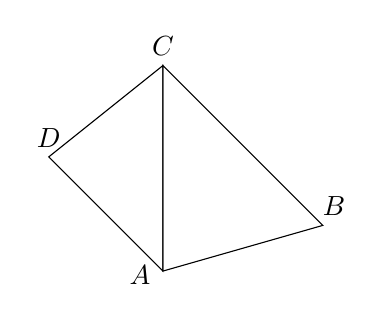
\begin{tikzpicture}[scale=0.29]
								\draw (0,0) -- (-5,5) -- (0,9) -- cycle;
								\draw (0,0) -- (7,2) -- (0,9) -- cycle;
								\coordinate[label=$A$] (A) at (-1,-1);
								\coordinate[label=$D$] (B) at (-5,5);
								\coordinate[label=$C$] (C) at (0,9);
								\coordinate[label=$B$] (D) at (7.5,2);
							\end{tikzpicture} 
							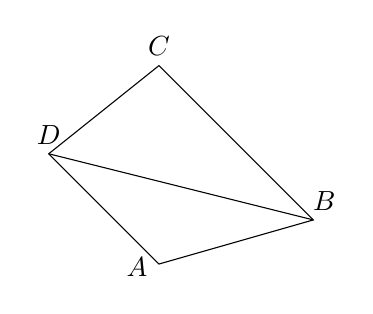
\begin{tikzpicture}[scale=0.28]
								\draw (0,0) -- (-5,5) -- (0,9) -- (7,2)-- cycle;
								\draw (-5,5) -- (7,2);
								%\draw (0,0) -- -- (0,9) -- cycle;
								\coordinate[label=$A$] (A) at (-1,-1);
								\coordinate[label=$D$] (B) at (-5,5);
								\coordinate[label=$C$] (C) at (0,9);
								\coordinate[label=$B$] (D) at (7.5,2);
							\end{tikzpicture}
							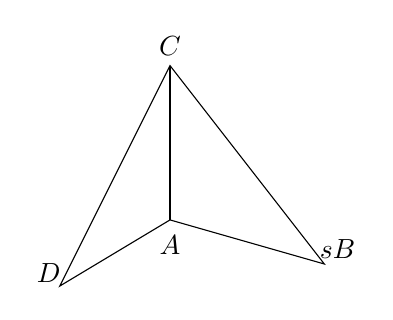
\begin{tikzpicture}[scale=0.28]
								\draw (0,0) -- (-5,-3) -- (0,7) -- (7,-2)-- cycle;
								\draw (0,0) -- (0,7);
								%\draw (0,0) -- -- (0,9) -- cycle;
								\coordinate[label=$A$] (A) at (0,-2);
								\coordinate[label=$D$] (B) at (-5.5,-3.3);
								\coordinate[label=$C$] (C) at (0,7);
								\coordinate[label=$sB$] (D) at (7.6,-2.2);
							\end{tikzpicture}
							
							From left to right a hinge $([ABCD],[AC])$, its flipping $([ABCD],[DB])$ and a non-convex hinge.
					\end{figure}
					\begin{defi}[Weighted hinge]\label{def:weighted_hinge}
						A weighted hinge is the datum of a hinge, $Q=([ABCD],[AC])$, and 
						a function $\tau:\{A,B,C,D\}\rightarrow\RR$.
					\end{defi}
					\begin{defi}[$\tau$-legal/$\tau$-critical hinge]\label{def:legal_critical_hinge} Let $(Q,\tau)$ be a weighted hinge. 
					Denote by $\tautilde{\tau}{Q}: Q \rightarrow \RR$ the distance-like function induced by the triangulation $\TT=([ABC],[ADC])$.
					A hinge $Q$ is $\tau$-legal (resp.\ $\tau$-critical, resp.\ $\tau$-illegal) if $\tautilde{\tau}{Q}$ is Q-convex (resp.\ $\mathscr C^1$, resp.\ strictly Q-concave) 					\end{defi}

					 
			

					Each edge $e$ of a given triangulation $\TT$ provides a hinge, indeed $e$ bounds two triangles $T_1,T_2\in \TT$ and the gluing of this two triangles along $e$ is a hinge. Beware that two such triangles might be actually the same in $\TT$ (a triangle glued to itself) but we take two copies to construct the hinge. More generally, we will need to consider immersed hinges.
					\begin{defi}\label{defi:immersed_hinge} An immersed hinge is a couple $(Q,\eta)$ with $Q$ a hinge  in $\E^2$ and $\eta: Q \rightarrow \Sigma$ an isometric
						immersion.		
						An immersed hinge $(Q,\eta)$ is embedded if the restriction  $\eta_{|Int(Q)}$ to the interior of $Q$ is an embedding.
					\end{defi}
					The hinge associated to an edge is embedded if and only if the triangles bounded by $e$ are different in $\TT$. 
					
					After an analysis of criteria ensuring $\tau$-legality of a given hinge, we notice the set of $\tau$ for which a given hinge is $\tau$-legal is the set of solutions of an affine inequality hence a convex set. Then we turn to the whole surface and try to construct triangulations for which all hinges are $\tau$-legal for a given $\tau$. 
					
					\begin{defi}[$\tau$-Delaunay triangulation]\label{def:delaunay_triangulation}
						Let $\TT$ be an adapted triangulation of $\Sigma$.

						The triangulation $\TT$ is $\tau$-Delaunay if the following equivalent properties are satisfied:
						\begin{enumerate}[(i)]
							\item $\tautilde{\tau}{\TT}$ is Q-convex;
							\item every hinge of $\TT$ is $\tau$-legal.
						\end{enumerate}
					\end{defi}
					For a given triangulation $\TT$, the set of $\tau\in\RR_ +^S$ such that $\TT$ is $\tau$-Delaunay is the set solutions of a system of affine inequalities hence a convex set (hence the first part of Theorem \ref{theo:domain_description}.$d$). However, $\adm$ is a possibly infinite union of such domains, therefore Theorem \ref{theo:domain_description}.$a$ and the second part of  point $d$ are not a direct Corollaries. We thus reverse the problem and construct a $\tau$-Delaunay triangulation with $\tau$ given a priori.
					
					The definition of $\tau$-Delaunay triangulation is coherent with the usual definition of Delaunay triangulation. Indeed, an adapted triangulation of $(\Sigma, S)$ is a subtriangulation of the Delaunay cellulation if and only if it is $0$-Delaunay. 
					The Delaunay cellulation can either be constructed as the dual of the Voronoi cellulation (see for instance of a thorough exposition \cite{MR1135877}) or via a flipping algorithm starting from a given adapted triangulation. The flipping algorithm is based upon the following remark (Lemma \ref{lem:inverse_Qstar}): for a given $\tau$, if a hinge is $\tau$-illegal then its flipping (if it exists) is $\tau$-legal. The algorithm then proceeds by flipping $\tau$-illegal hinges one by one in the hope that after finitely many iteration there won't be any $\tau$-illegal hinges left. Proposition \ref{prop:algo_stop} ensures the algorithm behaves mostly as expected: it stops after finitely many iterations on a triangulation without any flippable $\tau$-illegal hinges. To complete the analysis of the flipping algorithm, we show the resulting triangulation is $\tau$-Delaunay if and only if there exists such a triangulation. 
					
					We end the section applying the results obtained on the flipping algorithm to prove Theorem \ref{theo:domain_description}.







					\subsection{Q-convexity on hinges}\label{subsec:Qconvexhinge}


						Before going any further, we notice that the group $\isom(\E^2)$ acts naturally on weighted hinges and preserves legality.

						\label{sec:critere_Qconvexe}

						 In this subsection, we give ourselves a hinge
						 $Q=([ABCD],[AC])$ and some weights $\tau$. For simplicity sake, we choose a Cartesian coordinates system $(x,y)$ of $\E^2$, set $A=O$ the origin of this coordinate system and put $C$ on the vertical axis above $A$. Write $\omega$ and $\tau_0$ (resp.\ $\omega'$ and $\tau_0'$) the parameters given 
						 by Lemma \ref{lem:prolongement} on $[ABC]$ (resp.\ $[ADC]$) for the weights $\tau$;
						 define $$\function{\tau_{ABC}}{\E^2}{\RR}{x}{\tau_0-\d(x,\omega)^2} \quad \quad \function{\tau_{ADC}}{\E^2}{\RR}{x}{\tau_0'-\d(x,\omega')^2}.$$
						 
						The following picture sums-up the situation.
						\begin{center}
							\begin{tikzpicture}[scale=0.4]
								\draw (0,0) -- (-5,5) -- (0,9) -- cycle;
								\draw (0,0) -- (7,2) -- (0,9) -- cycle;
								\coordinate[label=$A$] (A) at (-1,-1);
								\coordinate[label=$D$] (B) at (-5,5);
								\coordinate[label=$C$] (C) at (0,9);
								\coordinate[label=$B$] (D) at (7.5,2);
								\draw [ style=dashed] (-10,4) -- (10,4);
								\draw [line width = 0.5pt](0.5,4) -- (0.5,4.5) -- (0,4.5);
								\draw (-2,4) node[above]{$\omega'$};
								\draw (-2,4) node{$\bullet$};
								\draw (6,4) node[above]{$\omega$};
								\draw (6,4) node{$\bullet$};
							\end{tikzpicture}
						\end{center}
                    \begin{rem}\label{rem:orth_omega}
						  Note that $\d(\omega,C)^2-\d(\omega,A)^2 = \d(\omega',C)^2-\d(\omega',A)^2 $
						hence $\overrightarrow{\omega\omega'} \perp \overrightarrow{AC}$. More generally, from the proof of Lemma \ref{lem:prolongement}, one sees that the orthogonal projection of $\omega$ on the line $(AC)$ only depends on $A,C$ and $\tau_A,\tau_C$.
						 \end{rem}
						\begin{prop}[Q-convexity criteria]\label{prop:Qconv_critere}
							Under this subsection hypotheses, the following are equivalent:
							\begin{enumerate}[(i)]
							 \item $\tautilde{\tau}{Q}$ is Q-convex;
							 \item $\tautilde{\tau}{Q}$ is Q-convex along some segment crossing $[AC]$;
							 \item $\tau_{ABC}\leq \tau_{ACD}$ on $[ACD]$ and $\tau_{ABC}\geq \tau_{ACD}$ on $[ABC]$.
							 \item $\tau_{ABC}(D)\leq \tau_{ACD}(D)$ or $\tau_{ABC}(B)\geq \tau_{ACD}(B)$.
							 
							 \item $x_{\omega}\geq x_{\omega'}$
							 \item
							 $$\left(\frac{y_B}{|x_B|}+\frac{y_D}{|x_D|}\right)\tau_C+\left(\frac{AC-y_B}{|x_B|}+\frac{AC-y_D}{|x_D|}\right)\tau_A\leq \frac{AC}{|x_D|}\tau_D+\frac{AC}{|x_B|}\tau_B+K$$
							 with
							 $$K=\frac{AC}{|x_B|}\left(AB^2-ACy_B\right)+\frac{AC}{|x_D|}\left(AD^2-ACy_D\right).$$
							\item Denoting by $\overrightarrow u\wedge \overrightarrow v$ the determinant $|\overrightarrow u \overrightarrow v|$:
							 $$\left(\overrightarrow{AB}\wedge\overrightarrow{AD}\right) \tau_C+\left(\overrightarrow{CD} \wedge\overrightarrow{CB}\right)\tau_A- \left(\overrightarrow{CA}\wedge \overrightarrow{CB}\right)\tau_D-\left(\overrightarrow{AC}\wedge \overrightarrow{AD}\right)\tau_B-K\leq 0$$
							 with
							 $$K=
							 \overrightarrow{AC}\wedge \overrightarrow{AD}
								\left(\overrightarrow{AB}\cdot \overrightarrow{CB}\right)
							 +
							 \overrightarrow{CA}\wedge \overrightarrow{CB}
								\left(\overrightarrow{AD}\cdot \overrightarrow{CD}\right)
							 .$$
							\end{enumerate}
						\end{prop}
						\begin{proof}
						

						 \begin{itemize}
							\item $(i)\Rightarrow (ii)$ is by definition.
							\item $(ii)\Rightarrow (i)$. Since the line $(\omega\omega')$ is perpendicular to $(AC)$ it follows that $\frac{\partial\tau_{ABC}}{\partial y} = \frac{\partial\tau_{ACD}}{\partial y} $, then $\overrightarrow\grad\,\tau_{[ABC]}-\overrightarrow\grad \tau_{[ACD]}$ is horizontal and the sign of $\langle \overrightarrow\grad\,\tau_{[ABC]}-\overrightarrow\grad \tau_{[ACD]}| \overrightarrow u\rangle$ does not depend on $\overrightarrow u$ as long as$\overrightarrow u$ is directed toward increasing $x$. 
							\item $(v)$ is equivalent to $\frac{\partial\tau_{ABC}}{\partial x} \geq \frac{\partial\tau_{ACD}}{\partial x}$ which is equivalent to Q-convexity along the direction perpendicular to $[AC]$. Hence, $(i)\Rightarrow (v)$ and $(v)\Rightarrow (ii)$.
							\item $(i)\Rightarrow (iii)$. Let $P\in [ABC]$, choose some $P'\in [ACD]$ such that $[P'P]$ crosses $[AC]$. The function $\tau_{[ACD]}$ is $\mathscr C^1$ while $\tautilde{\tau}{Q}$ is Q-convex along $[P'P]$. The same argument as in the proof of Lemma \ref{lem:diff_Q_convexe} gives the first inequality. The second is proven the same way. 
							\item $(iii)\Rightarrow(iv)$ is trivial.
							
							\item To prove $(iv)\Rightarrow (ii)$, consider any segment $[PB]$ with $P\in [ACD]$. Along such a segment, $\tautilde{\tau}{Q}$ is either Q-convex or strictly Q-concave. The inequality $\tau_{ABC}(B)\geq \tau_{ACD}(B)$ implies it is the former. The same argument shows $\tau_{ABC}(D)\leq \tau_{ACD}(D) \Rightarrow (ii)$.
							
						 \item $(v)\Leftrightarrow (vi)$ Solve explicitly the system in the proof of Lemma \ref{lem:prolongement} for both sides in $(v)$.
						 \item $(vii)$ is a geometric rewriting of $(vi)$ which can be checked by rewriting terms in coordinates.
						 \end{itemize}\end{proof}
						

						The previous Proposition shows Q-convexity is an affine constraint on $\tau$ for a given hinge. Since we will have to consider multiple hinges for multiple triangulations, we introduce the following.
						\begin{defi}[Affine form of a hinge] \label{defi:Q_forme_affine}

							Let $Q=([ABCD],[AC])$ be a hinge, define the affine form associated to $Q$ by:
							$$\function{Q^*}{\RR_+^{\{A,B,C,D\}}}{\RR}{\tau}{
								 \lambda_C\tau_C+
								 \lambda_A\tau_A
									-\lambda_D\tau_D-
									\lambda_B\tau_B-K
								 }
							$$
							where
							\begin{eqnarray*}
							 \lambda_C=\overrightarrow{AB}\wedge\overrightarrow{AD},&&\lambda_A=\overrightarrow{CD} \wedge\overrightarrow{CB},\\
							 \lambda_D=\overrightarrow{CA}\wedge \overrightarrow{CB},&&\lambda_B=\overrightarrow{AC}\wedge \overrightarrow{AD},
							\end{eqnarray*}
							 $$K= \overrightarrow{AC}\wedge \overrightarrow{AD}
								\left(\overrightarrow{AB}\cdot \overrightarrow{CB}\right)
							 +
							 \overrightarrow{CA}\wedge \overrightarrow{CB}
								\left(\overrightarrow{AD}\cdot \overrightarrow{CD}\right).$$
	
						
						
						\end{defi}
						\begin{rem}\label{rem:forme_linaire_Qconvexe} The affine form $Q^*$ is defined in such a way that $\tautilde{\tau}{Q}$
						is Q-convex if and only if $Q^*(\tau)\leq 0$.
						\end{rem}


						\begin{rem}\label{rem:immersed_hinge_sending_vertices}
						 If $(Q,\eta)$ is an immersed hinge of $(\Sigma, S)$ with $\eta$ sending vertices into $S$
						 and with $Q=([ABCD],[AC])$,
						 we can then define a corresponding affine form $\RR_+^{S}\rightarrow \RR$
						 $$\functionn{\RR_+^S}{\RR}{\tau}{Q^*(\tau\circ \eta_{|\{A,B,C,D\} }) }.$$
						 If there is no ambiguity we shall also denote it by $Q^*$.
						\end{rem}
						\begin{rem}\label{rem:hinge_critical_only} A hinge $Q$ is $\tau$-critical if and only if $Q^*(\tau)=0$.

						\end{rem}


						\begin{lem}\label{lem:inverse_Qstar}
				 Let $Q=([ABCD],[AC])$ be a flippable hinge and let $Q'$ its flipped hinge. 
				 As functions $\RR^{\{A,B,C,D\}}\rightarrow \RR$ we have:
				 
				 $$Q'^*=-Q^* $$
				\end{lem}
				\begin{proof}This can of course be checked directly in coordinates but we provide a more geometric proof.
					Following the notations of definition \ref{defi:Q_forme_affine} we write: 
					$$\function{Q^*}{\RR_+^{\{A,B,C,D\}}}{\RR}{\tau}{
								 \lambda_C\tau_C+
								 \lambda_A\tau_A
									-\lambda_D\tau_D-
									\lambda_B\tau_B-K
								 }$$ $$
					\function{Q'^{*}}{\RR_+^{\{A,B,C,D\}}}{\RR}{\tau}{
								 \lambda_C'\tau_C+
								 \lambda_A'\tau_A
									-\lambda_D'\tau_D-
									\lambda_B'\tau_B-K'
								 }
							$$
				where
							\begin{eqnarray*}
							 \lambda_C=\overrightarrow{AB}\wedge\overrightarrow{AD},&&\lambda_A=\overrightarrow{CD} \wedge\overrightarrow{CB},\\
							 \lambda_D=\overrightarrow{CA}\wedge \overrightarrow{CB},&&\lambda_B=\overrightarrow{AC}\wedge \overrightarrow{AD},\\
							 \lambda_D'=-\overrightarrow{BC}\wedge\overrightarrow{BA},&&\lambda_B'=-\overrightarrow{DA} \wedge\overrightarrow{DC},\\
							 \lambda_A'=-\overrightarrow{DB}\wedge \overrightarrow{DC},&&\lambda_C'=-\overrightarrow{BD}\wedge \overrightarrow{BA},
							\end{eqnarray*}
						We check that
					 $$ \lambda_A'=-\overrightarrow{DB}\wedge \overrightarrow{DC}
					 = -(\overrightarrow{DC}+\overrightarrow{CB})\wedge\overrightarrow{DC}
					 =-\overrightarrow{CB}\wedge \overrightarrow{DC} = -\overrightarrow{CD}\wedge \overrightarrow{CB}
					 = -\lambda_A$$
					 and we check the same way that $\lambda_B'=-\lambda_B$, $\lambda_C'=-\lambda_C$ and $\lambda_D'=-\lambda_D$.
					
					
					A quick way to prove that $K' = -K$ is to notice that 
					$$K = (AB\cdot CB\cdot CD \cdot DA) \sin\left(\widehat{BAD}+\widehat{DCB}\right) $$
					$$K' = (AB\cdot CB\cdot CD \cdot DA) \sin\left(\widehat{CBA}+\widehat{ADC}\right) $$
					and that $\widehat{BAD}+\widehat{DCB}+\widehat{CBA}+\widehat{ADC} = 0\,\mathrm{mod}\, 2\pi$\end{proof}






						\begin{cor}\label{cor:weighted_flippable_hinge_critical}
						 Let $(Q,\tau)$ be a weighted flippable hinge,
						 then $Q$ is $\tau$-critical if and only if its flipping $Q'$ is $\tau$-critical.
						\end{cor}

						\begin{cor} \label{cor:inversion_Qconvexe} Let $(Q,\tau)$ be a weighted flippable hinge and $Q'$ the flipping of $Q$.						
						If $Q$ is not $\tau$-critical, then the following are equivalent:
						\begin{enumerate}[(i)]
						 \item $Q$ is $\tau$-legal;
						 \item $Q'$ is $\tau$-illegal.
						\end{enumerate}
						\end{cor}


						\begin{lem}\label{lem:kernel_hinge} For any hinge $Q$, 
						 the indicator function $\mathbf{1}_S$ is in the kernel of the linear part of $Q^*$, e.g.\ 
						 $$\forall \tau\in \RR^S,\forall \lambda\in \RR, Q^*(\tau+\lambda\mathbf{1}_S)=Q^*(\tau).$$
						\end{lem}
						\begin{proof}
						 Using notations of Definition \ref{defi:Q_forme_affine}, we have
						 \begin{eqnarray*}
						 \lambda_A+\lambda_C-\lambda_B-\lambda_D &=& \overrightarrow{CD}\wedge \overrightarrow{CB} +\overrightarrow{AB}\wedge\overrightarrow{AD} - \overrightarrow{AC}\wedge \overrightarrow{AD}- \overrightarrow{CA}\wedge \overrightarrow{CB} \\
						 &=& \overrightarrow{AD}\wedge \overrightarrow{CB}+ \overrightarrow{CB}\wedge\overrightarrow{AD} \\
						 &=&0.
						 \end{eqnarray*}\end{proof}

						\begin{cor}\label{cor:translation}
							For all $\tau \in \adm$ and all $\lambda \in \RR$, 
							$$\tau+\lambda \mathbf{1}_S\in \adm \quad \Leftrightarrow \quad \tau+\lambda \mathbf{1}_S\geq 0.$$
						\end{cor}
						\begin{cor}\label{cor:theo3_b}
						With the notations of Theorem \ref{theo:domain_description},
							$$\adm = (\overline{\adm} + \RR\cdot\mathbf{1}_S)\cap \RR_+^S$$
						\end{cor}


					\subsection{Flipping algorithm}
										
						Let $\TT$ be an adapted triangulation of $(\Sigma, S)$. Consider $(Q,\eta)$ an immersed hinge given by an edge of $\TT$.
						We would like to flip $(Q,\eta)$ i.e.\ construct a new triangulation of $(\Sigma, S)$ with $\eta(Q)$ replaced by $\eta(Q')$ with $Q'$ the flip of $Q$.
 						There are three cases: 
						\begin{itemize}
						 \item if $\eta$ is not an embedding then the diagonal one wants to replace is also a side of the hinge. Hence, one cannot simply replace it without modifying the triangulation $\TT$ elsewhere;
						 \item if $\eta$ is embedded but $Q$ is not flippable.

						 \item if $\eta$ is embedded and $Q$ is flippable, then the flipped hinge $Q'$ is well-defined, $\eta: Q' \rightarrow \Sigma$ is well-defined, $\eta(Q')= \eta(Q)$ so that we only modify $\TT$ locally and the new triangulation $\TT'$ is composed of non degenerated triangles.
						\end{itemize}
					
						
						This remark motivates the following definitions.
						

						\begin{defi}[Flippable immersed hinge]\label{defi:immersed_hinge_flippable}
						An immersed hinge $(Q,\eta)$ is flippable if it is embedded and $Q$ is flippable; it is unflippable otherwise.
						\end{defi}


						
						\begin{defi}[Flipping algorithm]\label{def:flipping_algorithm}
							Let $\TT_0$ be any adapted triangulation of $(\Sigma, S)$ and let $\tau: S \rightarrow \RR_+$.
							The flipping algorithm proceeds as follows:
								\begin{enumerate}
								\item Set $i=0$.
								\item Let $L_i$ be the set of $\tau$-illegal flippable embedded hinges $(Q,\eta)$ induced by the edges of the current triangulation $\TT_i$.
								\item If $L_i$ is non-empty,
									\begin{enumerate}
										\item Choose some immersed hinge $(Q,\eta)$ in $L_i$.
										\item Replace the hinge $(Q,\eta)$ by its flipping $(Q',\eta)$ in $\TT_i$ to obtain a new
										triangulation $\TT_{i+1}$.
										\item increment $i$ and go to step $(2)$.
									\end{enumerate}
								\item If $L_i$ is empty, the algorithm stops and returns $\TT_i$.
							 \end{enumerate}
						\end{defi}
						The goal of the section is to prove the following.
						\begin{prop} \label{prop:algo_stop}
						 Let $\tau: S\rightarrow \RR_+$.
						 For any starting triangulation $\TT_0$, the flipping algorithm for $\tau$ starting at $\TT_0$
						 stops on some triangulation $\TT_\tau$ after finitely many iterations and every flippable immersed hinge in $\TT_\tau$ is $\tau$-legal. 
						 Furthermore, 
						 
						 \begin{itemize}
						 \item $\tau\in \adm$ if and only if $\TT_\tau$ is $\tau$-Delaunay;
						 \item $\displaystyle\max_\Sigma\tautilde{\tau}{\TT_\tau}\leq \max_S \tau + \max_\Sigma \tautilde{0}{\TT_0}$.
						 \end{itemize}
						\end{prop}
						\begin{rem}\label{rem:notation_last_proposition_consistent} The notation $\TT_\tau$ of this last Proposition is consistent with the one introduced in Definition \ref{defi:temps_admissbles}.
						 
						\end{rem}

						Two Lemmas are key to the proof, the first is Lemma \ref{lem:decroissante} which states that $\tautilde{\tau}{\TT_i}$ is decreasing along the iterations of the algorithm; the second is Lemma \ref{lem:arrete_ext} which implies that immersed unflippable hinges are always $\tau$-legal for $\tau\in \adm$, even those that are not associated to an edge. Lemma \ref{lem:arrete_ext} will be again useful in the following section.
												\begin{lem}\label{lem:decroissante}
						 Let $\tau: S \rightarrow \RR_+$ and let $\TT_0$ be an adapted triangulation. Let $(\TT_i)_{i\in I}$ be the sequence of triangulation given by 
						 the flipping algorithm with weights $\tau$ and starting at $\TT_0$, where
						 $I=\lsem 0,n\rsem$ or
						 $\NN$.

						 Then, the associated sequence of distance-like functions $(\tautilde{\tau}{\TT_i})_{i\in I}$ is decreasing:
						 \begin{itemize}
						 \item for all $i,j\in I$ with $i\leq j$ then $\tautilde{\tau}{\TT_i}\geq \tautilde{\tau}{\TT_j}$;
						 \item for all $i,j\in I$ with $i<j$ there exists $x\in \Sigma$ such that $$\tautilde{\tau}{\TT_i}(x)> \tautilde{\tau}{\TT_j}(x).$$
						 \end{itemize}
						\end{lem}
						\begin{proof} Let $i\in I$ such that $i+1\in I$.
						The triangulation $\TT_{i+1}$ is obtained from $\TT_i$ by flipping an embedded hinge, say $(Q,\eta)$ of $\TT_i$ with $Q=([ABCD],[AC])$.
						Then
						\begin{itemize}
						 \item $\forall x\in \Sigma\setminus \eta(Int(Q)),~~ \tautilde{\tau}{\TT_i}(x)=
						 \tautilde{\tau}{\TT_{i+1}}(x)$.
						Indeed, for $x\notin \eta(Q)$, the triangle containing $x$ is the same in $\TT_i$ and $\TT_{i+1}$.

						 \item $\forall x\in \eta(Int(Q)),~~ \tautilde{\tau}{\TT_i}(x)>\tautilde{\tau}{\TT_{i+1}}(x)$.
								Indeed, $\tautilde{\tau}{Q}$ and $\tautilde{\tau}{Q'}$ are equal on $[AB],[BC],[CD]$ and $[DA]$; by hypothesis
								$\tautilde{\tau}{Q}$ is strictly Q-concave and, from Lemma \ref{cor:inversion_Qconvexe}, $\tautilde{\tau}{Q'}$ is strictly Q-convex. Applying Lemma \ref{lem:diff_Q_convexe} on segments going from side to side of $[ABCD]$
								we obtain 
								$$\forall x\in Int(Q), \quad \tautilde{\tau}{Q} > \tautilde{\tau}{Q'}.$$
						\end{itemize}
						\end{proof}
						\begin{cor}\label{cor:flip_injective}
							No triangulation appears twice in the sequence $(\TT_i)_{i\in I}$ given by the flipping algorithm.
						\end{cor}

						\begin{lem}\label{lem:max_quad}
						Let $\widetilde\tau$ be a non-negative distance-like function on $(\Sigma, S)$, if $\widetilde\tau$ is $\mathscr C^1$ on some geodesic of length $\ell$ then $$\max\widetilde\tau \geq \frac{\ell^2}{4}$$
					
						\end{lem}

						\begin{proof}
						
						
						Let $c:[a,b]\rightarrow \Sigma$ be an arc length parameterization of such a geodesic and let $f:=\widetilde\tau\circ c$, we have $$\function{f}{[a,b]}{\RR}{x}{-x^2+\alpha x+ \beta}$$
						for some $\alpha,\beta\in \RR$. 
						Furthermore, $\widetilde\tau\geq 0$ thus that $f(a)\geq 0$ and $g(b)\geq 0$.
					
						 Define $u:[a,b]\rightarrow \RR$ the unique affine function such that $u(a)=f(a)$ and $u(b)=b$. We thus have $\forall x\in [a,b], f(x)=u(x)-(x-a)(x-b)$. 
						 On the one hand, $f(a)$ and $f(b)$ are non-negative so $u$ is non-negative.
						 On the other hand, $$\max_{x\in[a,b]}(-(x-a)(x-b))=\frac{(b-a)^2}{4}=\frac{\ell^2}{4}.$$ The result follows.
						 \end{proof}
						\begin{lem} \label{lem:triangulation_finie}
						For $C\in \RR_+^*$, let $E_C$ the set of adapted triangulations $\TT$ of $(\Sigma, S)$ such that $$\exists \tau\in \RR_+^S,\max\tautilde{\tau}{\TT}\leq C.$$
						Then, $E_C$ is finite.
						\end{lem}
						\begin{proof}
						 Let $\TT$ be an adapted triangulation such that $\exists \tau\in \RR_+^S,\max\tautilde{\tau}{\TT}\leq C$. Choose such a $\tau$. 
						 Let $e$ the longest edge of $\TT$. 
						 From Lemma \ref{lem:max_quad} with $L=\mathrm{length}(e)$
						 $$ \frac{L^2}{4} \leq\max_{e}\tautilde{\tau}{\TT} \leq C $$
						 thus $L\leq 2\sqrt{C}$. Therefore, the triangulation $\TT$ only has edges of length lesser than $2\sqrt{C}$.
						 
						 Consider a finite covering $\widehat\Sigma$ of $\Sigma$ branched above $S$ such that all cone angles of $\widehat\Sigma$ are bigger than $2\pi$. Note that $\widehat \Sigma$ is locally CAT(0) so 
						 its universal (unbranched) covering $\widetilde{\Sigma}$ is CAT(0) by Theorem 3.3.1 of \cite{alexander2019invitation} and hence for any two points in $\widetilde \Sigma$ above $S$, there exists at most one geodesic (see section  2.2 in \cite{alexander2019invitation}). 
						 Furthermore, any geodesic of length at most $2\sqrt{C}$ in $\Sigma$ from a point $A$ of $S$ to a point $B$ of $S$ lifts to a geodesic 
						 in $\widetilde \Sigma$ of same length  starting from a fixed $\hat A$ to some unfixed lift $\hat B$ of $B$ in the ball of radius $2\sqrt L$ around $\hat A$.
						 There are finitely many such $\hat B\in\widetilde \Sigma$, thus finitely such geodesics in $\widetilde \Sigma$. 
						 There are thus only finitely many geodesics of $\Sigma$ from $S$ to $S$ of length bounded by $2\sqrt{C}$, hence there are only finitely many triangulations with edges of length at most $2\sqrt{C}$. 
						\end{proof}

						\begin{lem} \label{lem:arrete_ext}
							Let $Q$ be an unflippable hinge with $Q=([ABCD],[AC])$.
							If there exists some distance-like Q-convex function $f$ on $[ABCD]$ extending $\tau: \{A,B,C,D\} \rightarrow \RR$, then $Q$ is $\tau$-legal.
						\end{lem}
						\begin{rem}\label{rem:beware_triangulations_may_very} Beware that $f$-triangulations of $[ABCD]$ may be very different from $([ABC],[ACD])$. 
						 
						\end{rem}

						
						\begin{proof}
							Without loss of generality, we may assume that $C$ is in the convex hull of 
							$[ABCD]$.
							Define $g:=\tautilde{\tau}{Q}$ and $h$ the 
							distance-like extension of $\tau_{|\{A,B,D\}}$ on $[ABD]$ given by Lemma \ref{lem:prolongement}.
							Both functions $f$ and $g$ are defined on $[ABCD]\subset [ABD]$ and $h$ is defined on $[ABD]$. Furthermore, $g$ is either Q-convex or Q-concave.
							
							Applying Lemma \ref{lem:diff_Q_convexe} on sides the hinge $Q$ then on any edge within $Q$ and with extremities on the sides, we see that $f\leq h$ and that either $h\geq g$ or $h\leq g$ depending on whether $g$ is  Q-convex or Q-concave.

							Since $g-h$ is affine on each triangle $[ACB]$ and $[ACD]$ and null at $A,B$ and $D$, we see that
							$g-h$ is non-positive	if and only if $g(C)-h(C)\leq 0$.
							However, $g(C)=f(C)\leq h(C)$, so $g\leq h$ hence $g=\tautilde{\tau}{Q}$ is Q-convex.
						\end{proof}
						\begin{lem} \label{lem:arrete_deg} Let $\tau:S\rightarrow \RR_+$ and 
						 let $(Q,\eta)$ be an immersed hinge with $Q=([AB_{-1}B_0B_{1}],[AB_0])$ such that $[AB_0B_{1}]$ is obtained from $[AB_{-1}B_0]$ via a rotation and $\eta([AB_0])=\eta([AB_1])=\eta([AB_{-1}])$.
						 
						Then, there exists an immersed hinge $(\hat Q,\hat\eta)$ with $\hat Q$ unflippable such that 
						$(Q,\eta)$ is $\tau$-legal if and only if $(\hat Q,\hat\eta)$ is $\tau$-legal.				
						\end{lem}
						\begin{proof} Let $\theta = \widehat{B_0AB_1}$ and $n=\lceil\pi/\theta\rceil-1$,
						if $\theta\geq \pi/2$ then take $\hat Q=Q$ and $\hat\eta=\eta$.
						
						 Otherwise, construct the polygon $[AB_{-n}\cdots B_0\cdots B_{n}]$, such that for each $k\in\lsem 1-n,n\rsem$, the triangle $[AB_kB_{k+1}]$ is obtained from $[AB_0B_{1}]$ via the rotation of center $A$ and angle $\alpha_k=k\theta$. Define $\hat Q:=[AB_nB_0B_{-n}]$ and $$\functiondeux{\hat\eta}{\hat Q}{\Sigma}{x\in [AB_{2k}B_{2k+1}]}{\eta(\rho_{-2\alpha_{k}}(x))}{x\in [AB_{2k-1}B_{2k}]}{\eta(\rho_{-2\alpha_{k}}(x))}$$ 
						 where $\rho_\beta$ denote the rotation of center $A$ and angle $\beta$. 
						 
						
						\def\sq{0.707106781}
						 \begin{center}
							\begin{tikzpicture}[scale=3]
								\draw (0,0) -- (-\sq,\sq) -- (0,1) -- cycle;
								\coordinate[label=$A$] (A) at (0,-0.2);
% 								\coordinate[label=$D$] (B) at (-5,5);
								\coordinate[label=$B_0$] (B) at (0,1);
								\coordinate[label=$B_{-1}$] (B) at (\sq,\sq);
								\coordinate[label=$B_{1}$] (B) at (-\sq,\sq);
								\coordinate[label=$B_{-2}$] (B) at (1.07,0);
								\coordinate[label=$B_{-3}$] (B) at (\sq,-\sq-0.2);
								\coordinate[label=$B_{2}$] (B) at (-1.1,0);
								\coordinate[label=$B_{3}$] (B) at (-\sq,-\sq-0.2);
% 								\coordinate[label=$B$] (D) at (7.5,2);
								\draw[black,cm={cos(45) ,-sin(45) ,sin(45) ,cos(45) ,(0 cm,0 cm)}] (0,0) -- (-\sq,\sq) -- (0,1) -- cycle;
								\draw[black,cm={cos(90) ,-sin(90) ,sin(90) ,cos(90) ,(0 cm,0 cm)}] (0,0) -- (-\sq,\sq) -- (0,1) -- cycle;
								\draw[black,cm={cos(90) ,-sin(90) ,-sin(90) ,cos(90) ,(0 cm,0 cm)}] (0,0) -- (-\sq,\sq) -- (0,1) -- cycle;
								\draw[black,cm={cos(135) ,-sin(135) ,sin(135) ,cos(135) ,(0 cm,0 cm)}] (0,0) -- (-\sq,\sq) -- (0,1) -- cycle;
								\draw[black,cm={cos(90) ,-sin(-90) ,sin(-90) ,cos(90) ,(0 cm,0 cm)}] (0,0) -- (-\sq,\sq) -- (0,1) -- cycle;
								\draw[black,dashed] (\sq,-\sq) -- (0,1) -- (-\sq,-\sq);
							\end{tikzpicture}
						\end{center}
						We have $\forall k\in \lsem -n,n\rsem,\hat\eta(B_k)=\eta(B_0)$ the weights $\tau \in \RR^S$ thus induce weights $\hat\tau:=\tau\circ \hat\eta$ such that $\hat\tau(B_{k})=\tau(B_0)=\hat\tau(B_1)=\hat\tau(B_{-1})$.
						For $I,J,K \in \{A,B_{-n},\cdots,B_n\}$, denote by $\omega_{[IJK]}$ the center of 
						$\tautilde{\tau}{[IJK]}$ and by $\omega_{[IJ]}$ the orthogonal projection of $\omega_{[IJK]}$ on the line $(IJ)$. From remark \ref{rem:orth_omega}, the orthogonal projection of $\omega_{[IJK]}$ on the line $(IJ)$ only depends on $\hat\tau(I),\hat\tau(J)$ and $[IJ]$; in other words $\omega_{[IJ]}$ does not depend on $K$.
						
						Since $\hat\tau(B_n)=\hat\tau(B_0)=\hat\tau(B_{-1})$, then $\omega_{[B_0B_n]}$ (resp.\ $\omega_{[B_0B_{-n}]}$) is the middle of $[B_0B_n]$ (resp.\ of $[B_0B_{-n}]$). Since the lengths $(AB_k)_{k\in \lsem -n,n\rsem}$ are equal, the perpendicular bissectors of $[B_0B_{-n}]$ and $[B_0B_{n}]$ intersect at $A$, therefore $\omega_{AB_{-n}B_0}$ is on the right of $\omega_{AB_{n}B_0}$ on the perpendicular to $(AB_0)$ at $\omega_{[AB_0]}$ if and only if $\omega_{[AB_0]}$
						 is on the ray $[AB_0)$. Hence, by Proposition \ref{prop:Qconv_critere}.($v$), the hinge $\hat Q$ is $\hat\tau$-legal if and only if $\omega_{[AB_0]}$ is on the ray $[AB_0)$.
						
						The same argument shows $Q$ is $\hat\tau$-legal if and only if $\omega_{[AB_0]}$ is on the ray $[AB_0)$. Finally, 
						$(Q,\eta)$ is $\tau$-legal if and only if $(\hat Q,\hat \eta)$ is $\tau$-legal.\end{proof}
						\begin{proof}[Proof of Proposition \ref{prop:algo_stop}]
							By Lemma \ref{lem:decroissante}, the sequence of distance-like functions given by the flipping algorithm is bounded above by the first of the sequence $\tautilde{\tau}{\TT_0}$. Since $\tautilde{\tau}{\TT_0}-\tautilde{0}{\TT_0}$ is affine on each triangle of $\TT_0$ it is bounded by its value on $S$ thus by $\max_S \tau$. 
							Hence, $\forall i,\tautilde{\tau}{\TT_i}\leq \max_S{\tau}+\max\tautilde{0}{\TT_0}$.
							By Lemma \ref{lem:triangulation_finie}, the flipping algorithm runs through a finite set of triangulation. Finally, by Corollary \ref{cor:flip_injective}, the algorithm reaches a given triangulation at most once and thus stops after finitely many steps, say $n\in \NN^*$. The algorithm stops when the set of flippable $\tau$-illegal hinges is empty, then $\TT_n$ has no flippable $\tau$-illegal hinges.
							
							If the final triangulation $\TT_n$ is $\tau$-Delaunay then by definition $\tau\in \adm$. Assume $\tau \in \adm$ and consider $(Q,\eta)$ some unflippable hinge of $\TT_n$. Either $\eta$ is an embedding, in which case the weighted hinge $(Q,\tau\circ \eta)$ satisfies the hypotheses of Lemma \ref{lem:arrete_ext} and the immersed hinge $(Q,\eta)$ is then $\tau$-legal; or $\eta$ is not an embedding in which case $(Q,\eta)$ satisfies the hypotheses of Lemma \ref{lem:arrete_deg}, the immersed hinge $(\hat Q,\hat \eta)$ provided by Lemma \ref{lem:arrete_deg} satisfies the hypotheses of Lemma \ref{lem:arrete_ext}, it is thus $\tau$-legal and so is $(Q,\eta)$. Finally, $\TT_n$ is $\tau$-Delaunay.
						\end{proof}
						
						
						

				
					\subsection{Description of the Domain of admissible times}


						We may interpret Lemma \ref{lem:arrete_ext} together with \ref{lem:arrete_deg} in the following way: if $\tau \in \adm$, then all unflippable immersed hinges of $(\Sigma, S)$ with vertices in $S$ are $\tau$-legal. Furthermore, Proposition \ref{prop:algo_stop} shows the converse: the flipping algorithm stops on a triangulation $\TT$ which flippable hinges are all $\tau$-legal, if all unflippable hinges of $(\Sigma, S)$ are $\tau$-legal, in particular those of $\TT$ are $\tau$-legal, hence $\TT$ is $\tau$-Delaunay.
						We thus proved the following


						\begin{prop}\label{prop:domaine_convexe}
						Let $\mathbf{UFlip}$ the set of unflippable immersed hinge of $(\Sigma, S)$ with vertices in $S$. Then:
						 $$\adm = \bigcap_{(Q,\eta)\in \mathbf{UFlip}} (Q^*)^{-1}(\RR_-)$$
						 in particular $\adm$ is a convex domain of $\RR_+^{S}$.
						\end{prop}
						\begin{rem}\label{rem:lemma_lem_charniere_type}
						 Lemma \ref{lem:charniere_type_existence} below implies that $\mathbf{UFlip}$ is non-empty. Meanwhile, we take the convention that the intersection is $\RR_+^S$ if $\mathbf{UFlip} =\emptyset$.
						\end{rem}

						\begin{prop}\label{prop:unique_q_convex_distance_like_extension}
						 For $\tau\in \adm$, if $\widetilde\tau$ is the unique Q-convex distance-like extension of $\tau$ to $(\Sigma, S)$ then
						 $$\widetilde\tau = \min_{\TT'} \tautilde{\tau}{\TT'} $$
						 where $\TT'$ runs through all adapted triangulations of $(\Sigma, S)$.
						\end{prop}
						\begin{proof}
						 Take any adapted triangulation $\TT$ of $(\Sigma, S)$ and consider $T$ a triangle of $\TT$. On $T$, $\tautilde{\tau}{\TT}$ is $\mathscr C^1$ while $\widetilde\tau$ is Q-convex. By Lemma \ref{lem:diff_Q_convexe}, $\widetilde\tau \leq \tautilde{\tau}{\TT}$ on $T$. 
						 The triangle $T$ is arbitrary, thus $\widetilde\tau \leq \tautilde{\tau}{\TT}$ on $\Sigma$. 
						\end{proof}

						
				\begin{prop}\label{prop:delaunay_interieur}
				 The indicator function $\mathbf{1}_S$ of $S$ is in the interior of $\adm$.
				\label{prop:penint}
				\end{prop}
				\begin{proof}
					To begin with, by Theorem 4.4 of \cite{MR1135877} each cell of the Delaunay cellulation $\Cell$ of $(\Sigma, S)$ is isometric to a polygon inscribed into a circle of $\E^2$ whose center is a vertex of the Voronoi cellulation.
					For any given cell $C$ of the Delaunay cellulation, with $R_C$ the radius and $\omega\in \E^2$ the center of the circumscribed circle of the image of a development $\D:C\rightarrow\E^2$, the function 
					$$\function{f}{C}{\RR_+}{x}{R_C^2-\d(\D(x),\omega)^2}$$
					is distance-like $\mathscr C^1$ on $C$ and $f(p)=0$ for any vertex $p$ of $C$ hence $f$ for any adapted subtriangulation $\TT$ of $\Cell$, $\forall x\in C,\tautilde{0}{\TT}(x)=f(\D(x))$. 
					
					Let $e$ be an edge of the Delaunay cellulation, let $C,C'$ be the two cells on each sides of $e$ and denote by $\widetilde C,\widetilde C'$ lifts in a covering branched above $S$ such that $\widetilde C\neq \widetilde C'$ and such that $\widetilde C\cap \widetilde C'=\widetilde e$ with $\widetilde  e$ a lift of $e$. Choose a development $\D$ of $\widetilde C\cup \widetilde C'$ by abuse of notation $\omega,\omega'$ denote the center of the image of 
					$\widetilde C$ and $ \widetilde C'$ respectively.
					
					Denote by $Q^*_{e,\TT}$ the affine form associated with the hinge of axis $e$ for any subtriangulation $\TT$ of $\Cell$.
					\begin{itemize}
					 \item Claim: $Q^*_{e,\TT}(0)\neq 0$.
					 
					  The claim is equivalent to $\omega\neq\omega'$.
					  Assume by contradiction that $\omega=\omega'$ then vertices of $\D(\widetilde C)\cup \D(\widetilde C')$ are cocyclic hence $C$ and $C'$ are in the same Delaunay Cell ie $C$ is glued to itself via $e$. 
					 
					 Without loss of generality we may assume that $\omega$ is on the side (inclusively) of $\D(\widetilde C')$, hence  $e$ is strictly longer than every other edges of $C$. We deduce that $C$ cannot be glued to itself via $e$. Contradiction.
					 
					 \item Claim: $Q^*_{e,\TT}(0)\leq 0$.
					 
					 We may assume that the hinge at $e$ is developed as in the figure above Proposition \ref{prop:Qconv_critere}. We take the notations of the proposition.  Notice that assuming condition $(v)$ is not satisfied,  either $B$ is in the interior of the circumscribed circle of $ACD$ or $D$ is in the interior of the circumscribed circle of $ABC$. This violates a caracterization of the Delaunay cellulation.
					\end{itemize}
                    
					Define $$\U:=\RR_+^S\cap \bigcap_{\TT\in \mathbf{D}}\bigcap_e {Q^*_{e,\TT}}^{-1}(\RR_-^*)$$
					where $\mathbf{D}$ is the set of adapted subtriangulations of the Delaunay cellulation and $e$ runs through the edges of the Delaunay cellulation. The intersection is finite since there are only finitely many such subtriangulations and edges.
					$\U$ is thus an open subset of $\RR^S_+$ which contains $\RR_+ \mathbf{1}_S$.
					
					We now show $\U\subset \adm$. Apply the flipping algorithm for some $\tau\in \U$ and starting from some $\TT_0\in \mathbf{D}$ of the Delaunay cellulation. Let $\TT_0,\cdots,\TT_n$ be the sequence of triangulations given by the flipping algorithm.
					By induction, we have  $\TT_0\in\mathbf{D}$ and assuming $\TT_k\in \mathbf D$ for some $k<n$ then the conditions $Q_{e,\TT_k}^*(\tau)<0$ ensure that the edges $e$ are $\tau$-legal thus not flipped hence $\TT_{k+1}\in \mathbf{D}$. 
				From Proposition \ref{prop:algo_stop}, the triangulation $\TT_n$ is such that all flippable hinges are $\tau$-legal. On the one hand, the edges of $\Cell$ are $\tau$-legal since $\tau\in \U$. On the other hand all hinges inside a cell of the Delaunay cellulation are flippable. Finally, all the edges of $\TT_n$ are $\tau$-legal and 
				$\U$ is a subset of $\adm$.
				\end{proof}

				
				In order to obtain a finite cellulation of $\adm$ as well as characterizing its boundary we prove his transverse compactness.
				By transverse compactness of $\adm$ we mean that the projection of $\adm$ into the hyperplane $\{\tau\in \RR^S~|~\sum_{s\in S}\tau(s) = 0 \}$ is compact. Note that, for instance, if $\adm $ was equal to the whole $\RR_+^S$ then it wouldn't be transversely compact in this sense. The proof that $\adm$ is transversely compact relies upon the construction of affine constraints of the form $\tau_A-\tau_C\leq \varepsilon (\tau_A+\tau_B+\tau_C+\tau_D) + K$ with $\varepsilon>0$ arbitrary small and $A,C$ arbitrary in $S$.
				Such constraints are provided by type $(x,L)$ hinges, see Definition \ref{defi:charniere_type}, via Lemma \ref{lem:charniere_type_rel}. Lemma \ref{lem:charniere_type_existence} focuses on the construction of such immersed hinges.

				\begin{defi}[Type $(x,L)$ hinge]\label{defi:charniere_type}
					Let $x,L>0$, a hinge $([ABCD],[AC])$ of $\E^2$ is of type $(x,L)$ if it is non-convex with $C\in [ABD]$
					and \begin{eqnarray*}
					 \d(B,\Delta)\leq x,&& \d(D,\Delta)\leq x\\
							AB>L,&& AD>L
					 \end{eqnarray*}
					 where $\Delta$ is the line $(AC)$.
				\end{defi}

				\begin{lem}\label{lem:charniere_type_rel} Let $l>0$ and $x>0$.
				For all hinge $Q$, write
				$$Q^*:\tau \mapsto \alpha(Q)\tau_A+\beta(Q)\tau_B+\gamma(Q)\tau_C+\delta(Q)\tau_D+K(Q)$$
				associated affine form $Q$.

				Then, for all sequence $(Q_n)_{n\in \NN}$ of hinges
				such that for all $n\in \NN$, $Q_n$ is of type $(x,n)$ and axis length $l$ we have:
				\begin{eqnarray*}
				 \lim_{n\rightarrow +\infty} \frac{\alpha(Q_n)}{\gamma(Q_n)}= -1&\quad\quad&\displaystyle
				 \lim_{n\rightarrow +\infty} \frac{\beta(Q_n)}{\gamma(Q_n)}= 0\\
				 \lim_{n\rightarrow +\infty} \frac{\delta(Q_n)}{\gamma(Q_n)}= 0&&\forall n\in\NN,\,\gamma(Q_n)>0
				\end{eqnarray*}
				\end{lem}
				\begin{proof} Let $L>0$,
				and let $Q=([ABCD],[AC])$ be a hinge of type $(x,L)$ such that $AC=l$.
				 Whithout loss of generality, we may choose Cartesian coordinates of $\E^2$ such that $A:(0,0)$ is the origin,
				 $C:(0,l)$, $x_B>0$ and $x_D<0$.

				 There exists some $\lambda>0$ such that
				 \begin{eqnarray*}
					\beta(Q)=\lambda\frac{l}{|x_B|}&\quad\quad& \alpha(Q)=\lambda\left(\frac{l-y_B}{|x_B|}+\frac{l-y_D}{|x_D|} \right)\\
					\delta(Q) = \lambda\frac{l}{|x_D|} &\quad\quad & \gamma(Q)=\lambda\left(\frac{y_B}{|x_B|}+\frac{y_D}{|x_D|}\right) \\
				 \end{eqnarray*}

				We have $|x_B|\leq x$, $|x_D|\leq x$, $y_B\geq \sqrt{L^2-x^2}$ and $y_D\geq \sqrt{L^2-x^2}$;
				 thus $\gamma(Q)>0$ and $$ -1\leq\frac{\alpha(Q)}{f(Q)}\leq -1+ \frac{l}{\sqrt{L^2-x^2}}$$
				 $$ 0\leq\frac{\beta(Q)}{\gamma(Q)}\leq \frac{l}{\sqrt{L^2-x^2}} \quad 0\leq\frac{\delta(Q)}{\gamma(Q)}\leq \frac{l}{\sqrt{L^2-x^2}}.$$
				The result follows.
				\end{proof}
				\begin{lem}\label{lem:charniere_type_existence}
				 	Let $e$ be non-trivial geodesic segment of $(\Sigma, S)$ going from some $\sigma_1 \in S$ to some $\sigma_2\in S$ whose relative interior is in $\Sigma^*$.

				 	There exists $x_0>0$ such that for all $L>0$, there is an immersed hinge
				 	$Q=([ABCD],[AC],\eta)$ of type 
				 	$(x_0,L)$ such that $\eta([AC])=e$.
				\end{lem}
				\begin{proof}
				 Let $M:= \max_{x\in \Sigma} \d(x, S)$ and $m:=\min_{s\in S} \min _{s'\in S\setminus\{s\}}\d(s,s')$.
				 
				 Define $\Phi: \U\rightarrow \Sigma$ as the exponential map at $\sigma_1$ defined on some maximal star shaped open neighborhood $\U$ of $0$ in the tangent plane $T_{\sigma_1}\Sigma$ above $\sigma_1$ such that $\Phi(\U\setminus \{0\})\subset \Sigma\setminus S$. We identify $T_{\sigma_1}\Sigma$ with $\E^2_\alpha$ where $\alpha$ is the cone angle at $\sigma_1$ so that $\Phi$ is an isometric immersion from an open of $\E^2_\alpha$ to $\Sigma$. We choose polar coordinates $(r,\theta)$ of $\E^2_\alpha$ so that the direction $\theta=0$ is the initial derivative of the segment $e$. 
				 
				 With $\beta=\min(\alpha/2,\pi/6)$ define \begin{eqnarray*}r_{\max}&:&
				 \functionn{]-\beta,\beta[}{\RR_+^*\cup\{+\infty\}}{\theta}{ \max \{r \in \RR_ + ~|~ (r,\theta) \in \U \}}
				 \\R_{\pm}&:& \functionn{]0,\beta[}{\RR_+^*\cup\{+\infty\}}{\theta}{\min_{\theta'\in ]0,\theta]} r_{\max}(\pm\theta')}. 
				 \end{eqnarray*}

				 For any given $\theta \in ]-\beta,\beta[$, if $r_{\max}(\theta)<+\infty$ we extend $\Phi$ continuously to $(r_{\max}(\theta),\theta)$; note that in this case $\Phi(r_{\max}(\theta),\theta)\in S$.
				 
% 				 Let $r < \lim _{\theta \rightarrow 0^+}R(\theta)$, the curves $[0,r]\rightarrow \Sigma, s \mapsto \Phi(s,\theta_0)$ are well-defined for $\theta_0\in ]0,\beta[$ small enough. Furthermore, as $\theta_0$ goes to $0$ they converges uniformly toward a curve $c_0: [0,r]\rightarrow \Sigma$. The curve $c_0$ is the left geodesic of $\Sigma$ starting at $\sigma_1$ and such the $c_0'(0)=e'(0)$: 
% 				 \begin{itemize}
% 				 \item $c_0$ is a piecewise $\mathscr C^1$ curve geodesic on $\Sigma\setminus S$ , 
% 				 \item for all $t_0\in [0,r]$, with $\gamma$ the cone angle of $\Sigma$ at $c(t_0)$, the angle between $\lim_{t\rightarrow t_0^+}c'(t)$ and $-\lim_{t\rightarrow t_0^-}c'(t)$ is equal to $\pi$ mod $\gamma$.
% 				 \end{itemize} 
% 				Consequently, we continuously extend $\Phi$ to $\{(r,0)~:~ r< \lim_{\theta\rightarrow 0^+} R(\theta)\}$.
% 				
% 				 
				\begin{claim}\label{claim:claim}{$\limsup_{\theta\rightarrow 0^+} \theta R_\pm(\theta)\leq 2M$.}
				\end{claim}
				 \\ Let $\theta\in ]0,\beta[$, $\Phi$ is defined on the interior the triangle $[OAB]\subset \E^2_{\alpha}$ with $A=(R_+(\theta),0)$ and $B=(R_+(\theta),\theta)$ in polar coordinates. The inscribed circle of $[OAB]$ bounds an open disc whose image by $\Phi$ does not contain any element of $S$, hence the radius $\frac{1}{2}R_+(\theta)\left(\cos(\theta)+\sin(\theta)-1)\right)$ of this inscribed circle is lesser than $M$. One easily checks that $\cos(\theta)+\sin(\theta)-1\sim_{\theta \rightarrow 0^+} \theta$. The result follows for $R_+$ and one may proceed the same way for $R_-$.

				\begin{claim}\label{claim:claim_2}{$\lim_{\theta\rightarrow 0^+} R_\pm(\theta)= +\infty$.}
				\end{claim}\\
					The function $R_+$ is non-decreasing by definition so the limit is well-defined. Define a sequence $(\theta_n)_{n\in\NN}$ as follows: choose some $\theta_0\in]0,\beta[$ such that $r_{\max}(\theta_0)=R_+(\theta_0)$ and $\sin(\theta_0)\leq m/2$, then for all $n\in\NN$ take $\theta_{n+1}\in]0,\theta_{n}/2[$ such that $r_{\max}(\theta_{n+1})=R_+(\theta_{n+1})$. The map $\Phi$ can be continuously extended to the domain $$D:=\bigcup_{n\in\NN}\left\{(r,\theta)~:~\theta \in [0,\theta_n], r\leq R(\theta_n)\right\}.$$
					Write $P_n:=(R_+(\theta_n),\theta_n)$; since $\forall n\in\NN,\Phi(P_n)\in S$, then for all $n\in\NN$,
					$$R_+(\theta_{n+1})-R_+(\theta_n)+\theta_n-\theta_{n+1} =\d_D(P_n,P_{n+1})\geq \d_\Sigma(\Phi(P_n),\Phi(P_{n+1}))\geq m,$$ thus 
					$$\forall n\in\NN,\quad R_+(\theta_{n})\geq nm + R_+(\theta_0)+\theta_0-\theta_n\xrightarrow{n\rightarrow +\infty} +\infty$$
					One may proceed the same way for $R_-$.
									\def\sq{0.707106781}
				\def\myrad{6cm}% radius of the circle
				\def\deltarad{1cm}
				\def\deltatheta{7}% angle for the arc
				\def\thetamax{30}
						 \begin{center}
							\begin{tikzpicture}[scale=1]
								\coordinate (O) at (0,0);
% 								\draw (0,0) -- (-\sq,\sq) -- (0,1) -- cycle;
								\draw (\thetamax:\myrad) coordinate (slcoord) -- (\thetamax:0);
								\draw 
									(\thetamax-\deltatheta:\myrad) coordinate (slcoord) arc[start angle=\thetamax-\deltatheta,end angle=\thetamax,radius=\myrad];
								\draw (\thetamax-\deltatheta:\myrad) coordinate (slcoord) -- (\thetamax-\deltatheta:\myrad+\deltarad);
								\draw 
									(\thetamax-2*\deltatheta:\myrad+\deltarad) coordinate (slcoord) arc[start angle=\thetamax-2*\deltatheta,end angle=\thetamax-\deltatheta,radius=\myrad+\deltarad];
								\draw (\thetamax-\deltatheta:\myrad) coordinate (slcoord) -- (\thetamax-\deltatheta:\myrad+\deltarad);
								\draw 
									(\thetamax-3*\deltatheta:\myrad+2*\deltarad) coordinate (slcoord) arc[start angle=\thetamax-3*\deltatheta,end angle=\thetamax-2*\deltatheta,radius=\myrad+2*\deltarad];
								\draw (\thetamax-2*\deltatheta:\myrad+\deltarad) coordinate (slcoord) -- (\thetamax-2*\deltatheta:\myrad+2*\deltarad);
								\draw[dashed]
									(0:\myrad+3*\deltarad) coordinate (slcoord) 
									arc[start angle=0,end angle=\thetamax-3*\deltatheta,radius=\myrad+3*\deltarad];
									
								\draw (\thetamax-3*\deltatheta:\myrad+2*\deltarad) coordinate (slcoord) -- (\thetamax-3*\deltatheta:\myrad+3*\deltarad);
								
								\draw (0,0) -- (\myrad+4*\deltarad,0);
								\coordinate[label=$O$] (O) at (0:0) coordinate (slcoord);
								\coordinate[label=$P_0$] (A) at (\thetamax:\myrad) coordinate (slcoord);
								\coordinate[label=$P_1$] (B) at (\thetamax-\deltatheta:\myrad+\deltarad) coordinate (slcoord);
								\coordinate[label=$P_2$] (C) at (\thetamax-2*\deltatheta:\myrad+2*\deltarad) coordinate (slcoord);
								\coordinate[label=$P_3$] (D) at (\thetamax-3*\deltatheta:\myrad+3*\deltarad) coordinate (slcoord);

% 									;
% 								\coordinate[label=$A$] (A) at (0,-0.2);
% 								\coordinate[label=$B$] (D) at (7.5,2);
% 								\draw[black,cm={cos(45) ,-sin(45) ,sin(45) ,cos(45) ,(0 cm,0 cm)}] (0,0) -- (-\sq,\sq) -- (0,1) -- cycle;

							\end{tikzpicture}
						\end{center}
					
				We now come back to the proof of the Lemma. Take some $x_0>M$, for any $L\in \RR_+$, from the claims above, there exists some $\theta_+\in]0,\beta[$ and $\theta_-\in ]-\beta,0[$ such that $|\sin(\theta_\pm)r_{\max}(\theta_\pm)| \leq x_0 $ and $r_{\max}(\theta_{\pm})\geq L$. Choose such a $\theta_\pm\in ]-\beta,\beta[$ and notice $\Phi$ is well-defined on the hinge
				$Q=[ABCD]$ with $A=O$ $B:=(r_{\max}(\theta_-),\theta_-)$, $C:=(\mathrm{len}(e),0)$ and $D:=(r_{\max}(\theta_+),\theta_+)$. The hinge $Q$ is of type $(x_0,L)$ and $\eta:= \Phi_{|Q}$ is an isometric immersion. The immersed hinge $(Q,\eta)$ is then of type $(x_0,L)$ with vertices in $S$ and such that $\Phi([AC])=e$.\end{proof}



				\begin{lem} \label{lem:admissible_compact}
					There exists $C>0$ such that for all $A,B\in S$ and all $\tau\in \adm$, $$|\tau(A)-\tau(B)|\leq C.$$

					\end{lem}
					\begin{proof}
						From Corollary \ref{cor:translation}, it is enough to find a $C>0$ such that 
						$$\forall \tau\in \adm,\quad \min\tau=0~\Rightarrow~ \max \tau\leq C$$
					
					From Lemmas \ref{lem:charniere_type_rel} and \ref{lem:charniere_type_existence} and from Proposition \ref{prop:domaine_convexe},
						for all $\varepsilon>0$, and $A,B\in S$, if there exists a geodesic from $A$ to $B$ whose relative interior is in $\Sigma\setminus S$, then there exists $K>0$ such that $\forall\tau\in \adm, \left|\tau_A-\tau_B\right| \leq \varepsilon \max \tau +K $.
						For all $A,B\in S$ there exists a geodesic from $A$ to $B$ possibly intersecting $S$ in his relative interior hence 
						$$\forall \varepsilon>0,\forall A,B\in S,\,\exists K>0,\quad \mathrm{s.t.}\quad \forall \tau \in \adm,\, |\tau_A-\tau_B|\leq \varepsilon \max \tau + K $$

						Since $S$ is finite, 
						$$\exists K>0,\forall A,B\in S,\forall \tau\in \adm,\quad |\tau_A-\tau_B|\leq \frac{1}{2}\max \tau +K$$

						Choose such a $K>0$ and define $C=2K$, then for all $\tau\in \adm$ such that $\min \tau=0$
						 $$\max \tau = |\max \tau-\min\tau| \leq \frac{1}{2} \max\tau +K $$
						thus for such a $\tau$
						
						$$\max \tau \leq 2K = C.$$\end{proof}

					\begin{proof}[Proof of Theorem \ref{theo:domain_description}]
						Let $\pi$ be the orthogonal projection of $\RR^S$ onto $H:=\{\tau\in \RR^S~|~ \sum_{s\in S}\tau(s)=0\}$, note that the kernel of $\pi$ is $\RR\cdot \mathbf{1}_S$. 
						For each triangulation $\TT$, the set of $\tau\in \RR_+^S$ such that $\tautilde{\tau}{\TT}$ is Q-convex is the domain $$\CellPSigma:= \RR_+^S\cap \bigcap_{e \in \mathrm{Edge(\TT)}} (Q_e^*)^{-1}(\RR_-).$$
						Since $\mathbf{1}_S$ is in the kernel of the linear part of all the affine form $Q^*_e$ and since the number of edges of $\TT$ is finite, $\overline \CellPSigma:= \pi(\CellPSigma)$ is a convex polyhedron and $\CellPSigma = (\overline \CellPSigma +\RR\cdot \mathbf{1}_S)\cap \RR_ +^S$.
						
						On the one hand, $$\adm = \bigcup_{\TT}P_{\TT}$$ where $\TT$ runs through all adapted triangulations of $(\Sigma, S)$. Then defining $\overline{\adm}:= \bigcup_{\TT}\overline{\P}_{\TT}$ we have $\adm= (\overline{\adm} + \RR\cdot\mathbf{1}_S)\cap \RR_+^S$.
						
						On the other hand, by Lemma \ref{lem:admissible_compact}, $\overline \adm = \pi(\adm)$ is compact. Furthermore, by Proposition \ref{prop:domaine_convexe}, $\adm$ is convex hence $\overline \adm$ is convex. 
						
						Then, consider the set $\mathbf {T}$ of triangulations that are $\tau$-Delaunay for some $\tau\in \adm$. 
						For any admissible $\tau\in \adm$ it follows from Lemma \ref{lem:kernel_hinge}  that $\tau':=\tau-\min\tau \in \adm$ and that the set of $\tau$-Delaunay triangulations is equel to the set of $\tau'$-Delaunay triangulations. 
						Therefore, $\mathbf T$ is the set of triangulations that are $\tau$-Delaunay for some $\tau\in \adm_0 := \{\tau \in \adm~|~ \min\tau=0\}$.
						By Lemma \ref{lem:admissible_compact}, there exists a constant $C$ that only depends on $\Sigma$ such that  $\forall \tau\in \adm_0,\tau\leq C$. By Proposition \ref{prop:algo_stop}, there thus exists a constant $A$ that only depends on $\Sigma$ such that $\tautilde{\tau}{\TT}\leq A$ for all $\tau$-Delauney triangulation $\TT$ and all $\tau\in \adm_0$. Using notations of  Lemma \ref{lem:triangulation_finie}, we deduce that $\mathbf T \subset E_A$ which is finite hence $\mathbf T$ is finite. 
						The domain $\overline \adm$ is thus a polyhedron. 
						 
                        Choose any triangulation $\TT_0$ and define $A:=\sup_{\tau\in \adm_0} \max_{x\in \Sigma} \tautilde{\tau}{\TT_0}(x)$; by compactness of $\overline \adm$,  the set $\adm_0$ is bounded hence $A< +\infty$.                        
                        Consider the finite family $(Q_i)_{i\in \lsem 1,q\rsem}$ of unflippable immersed hinges around edges of triangulations in $E_A$ and define $\adm_A:= \bigcap_{i=1}^{q} {Q_i^*}^{-1}(\RR_-)$. 
                        By Proposition \ref{prop:domaine_convexe} we have $\adm_A\supset \adm$. In addition, for any $\tau\in \adm_A$ the flippling algorithm starting at  $\TT_0\in E_A$ stops after finitely many iterations on some $\TT_n\in E_A$; Proposition \ref{prop:algo_stop} ensures that flippable hinges of $\TT_n$ are $\tau$-legal and the definition of $\adm_A$ ensures that unflippable hinges of $\TT_n$ are also $\tau$-legal; we deduce that $\TT_n$ is $\tau$-Delaunay hence $\tau\in \adm$. We conclude that $\adm=\adm_A$, so that essential support planes of $\adm_A$ are either 
                        \begin{itemize}
                         \item essential support planes of $\RR_+^S$ thus of the form $\tau_\sigma=0$ for some $\sigma\in S$,
                         \item or given by ``$Q_i^*=0$" for some $i\in \lsem 1,q\rsem$.
                        \end{itemize}
                        Finally, since $\adm$ is a finite union of cells, essential support planes of the second kind correspond to a facet of some cell $\adm_\TT$. 
                        Point  (e) of Theorem \ref{theo:domain_description} follows.\end{proof}

			\section{Volkov Lemma for Lorentzian Convex cones}
				\label{sec:etude_domaine_convexe_bord}
				
				
                 In effective methods used to prove Alexandrov-like Theorems, at some point is needed a Volkov Lemma bounding the cone angle $\Theta$ around a singular line of angle $\kappa$ in a Riemannian manifold. This is used to exclude some positions of critical points of the Einstein-Hilbert functionnal introduced in the following section.
    
                
                In our work, we consider spacelike convex cones in $\mass{\kappa},\kappa>0$ eg the model space of the timelike singular lines of angle $\kappa$ as $\RR^3$ endowed with the metric $\d t^2-\d r^2-\left(\frac{\kappa}{2\pi}\right)^2\d \theta^2$.               
                There are many ways to rigorously define a spacelike cone in $\mass{\kappa}$. In out context we define a cone $\D$ as  the graph of some Lipchitz 1-homogeneous function $t : \RR^2 \mapsto \RR$, the cone is spacelike if the graph in $\RR^3$ identified to $\mass{\kappa}$ is spacelike. The cone $\D$ is then convex if the future $J^+(\D)$  is convex in the sense that any spacelike geodesic with extremities in $J^+(\D)$ is in $J^+(\D)$. 
				The Lorentzian structure of $\mass{\kappa}$ induces complete metric space structure on the cone which is locally Euclidean except possibly at $\{r=0\}$. In other words, $\D$ is isometric to $\E^2_\Theta$ for some $\Theta>0$, this $\Theta$ is its so-called cone angle.
				
				
				
				
				
% 				As we shall see, the Riemannian and Lorentzian cases are essentially equivalent, the role of $\Theta$ and $\kappa$ being simply exchanged.
				
			
			
				
				
				
				
				
				Let $\D$ be a cone defined as the graph of $t:\RR^2\rightarrow \RR$. A {\it wedge} is the graph of $t$ on some domain $\{\theta\in I\}$ with $I$ an interval, such a wedge is {\it coplanar} if it is totally geodesic. A wegde is isometric to some domain $\{(r,\theta)~:~r\geq 0, 0\leq \theta \leq \pi \}$ in $(\RR^2,\d r^2+ (\frac{\alpha }{\pi} )^2r^2 \d \theta^2)$; the value of $\alpha$ is unique and we refer to it as the {\it Euclidean angle} of the wedge.
				
				\begin{theo}\label{theo:volkov_lorentz} Let $\Theta>0$ and $\kappa>0$. Let $\Cone$ be a convex spacelike cone in $\mass{\kappa}$ of cone angle $\Theta$ whose vertex is on the singular line of $\mass{\kappa}$. 
					
					 Assuming $\Cone$ has a coplanar wedge of Euclidean angle at least $\min(\pi,\Theta)$:

					\begin{itemize}
					 \item if $\Theta> 2\pi$ then $\kappa > 2\pi$.;
					 \item if $\Theta = 2\pi$ then $\kappa = 2\pi
					 $;
					 \item if $\Theta\in ]\pi,2\pi[$ then $\kappa \geq \Theta$;
					 \item if $\Theta = \pi$ then $\kappa = \pi$;
					 \item if $\Theta<\pi$ then $\kappa\in ]0,\Theta]$ with $\kappa=\Theta$ if and only if $\Cone$ is the horizontal plane;
					\end{itemize}
					and all the bounds above are sharp.
					\end{theo}
                \begin{rem}\label{rem:though_results_stated_above}
                 Though results such as stated above are used one way or another in \cite{MR2127379,MR2410380,MR2453328,MR2469522,MR2813423,milka1996space}, to our knowledge a complete proof of the bounds we use is not available in English (one may appear in the original thesis of Volkov which is in Russian and only a summary is available in English \cite{MR3904042}), we thus provide a complete proof. 
                \end{rem}               

					
				\begin{rem}\label{rem:minkowski_convex_cone_always} In Minkowski, a convex cone always has a cone angle bigger than $2\pi$. One may expect this to carry out in $\mass{\kappa}$ for arbitrary $\kappa\geq0$. Theorem \ref{theo:volkov_lorentz} shows this intuition is valid for $\kappa \in [0,\pi]\cup\{2\pi\}$ but not for $\kappa\in ]\pi,2\pi[$.			 
				\end{rem}

                    When considering a cone $\mathcal D$ in $\E^3$, an elementary remark is that the angle of the conical singularity is in fact the length of its {\it stalk}: the curve given by the intersection $\D\cap \SS^2$. By extension ''stalk`` refers to curves in $\SS^{2}$ or $\SS^{1,1}$ that are graphs over the ''equator``. 
					As in the Euclidean case, we may notice that the angle $\Theta$ of the conical singularity of a spacelike cone in $\mass{\kappa}$ is given by the length of the spacelike curve induced on $\SS^{1,1}_\kappa:=\{(t,x,y) \in \mass{\kappa}~|~ r^2-t^2=1\}$. However, the relation between $\kappa$ and $\Theta$  is far from trivial and the Lorentzian nature of $\SS^{1,1}$ does not help. One may devise an analytical proof of the needed Volkov Lemma \cite{thesis} but a more geometrical one is provided based on a suggestion of Graham Smith. 
					
					The key idea developed in section \ref{sec:stalks} is that to each cone stalks $\rho : \RR/\kappa\ZZ \rightarrow \SS^{1,1}_\kappa$ corresponds a dual stalk $\gamma : \RR/\Theta\ZZ \rightarrow \SS^2_\Theta$. The length of $\rho$ is the Euclidean cone angle $\Theta$ while the length of $\gamma$ is the Lorentzian cone angle $\kappa$.
				
				\subsection{Stalks of Lorentzian cones} \label{sec:stalks}
					Although we defined cones with Lipchitz regularity, we will focus our argumentation on polyhedral cones that are simpler to describe. A density argument allowing to generalize to lower regularity.
					
					\begin{defi}[Stalk of a spacelike cone]\label{def:stalk_spacelike_cone}
					Let $\kappa>0$, $\Theta>0$ and $\Cone$ a spacelike cone of $\mass{\kappa}$ of cone angle $\Theta$.
					In cylindrical coordinates $(r,\theta, t)$, the set $\SS^{1,1}_\kappa\cap \Cone$ can be parameterized by arc length with increasing $\theta$ coordinate
					$$\Cone\cap \SS^{1,1}_\kappa= \left\{ \left(\begin{array}{c}
						t(s)\\
						r(s)\\
						\theta(s)
					\end{array}\right) ~:~ s\in \RR\right\}.
					$$
					The stalk $\rho_{\Cone}$ of $\Cone$ is the function $ t: \RR\rightarrow \RR$ of this parameterization.
					\end{defi}
					\begin{rem}\label{rem:stalk_cone_unique_up}
					 The stalk $\rho$ of a cone is unique up to pre-composition by an affine transformation slope $\pm1$.
					\end{rem}




					\begin{prop}\label{prop:T_convexe_base}
					Let $\kappa>0$, $\Theta>0$ and $\Cone$ a cone of $\mass{\kappa}$ of cone angle $\Theta$ whose vertex is on the origin and of stalk $\rho:=\rho_{\Cone}$. We have the following:
					\begin{enumerate}
					\item $\rho: \RR \rightarrow \RR$ is $\Theta$-periodic and Lipchitz continuous;
					\item $\D$ is polyhedral if and only if $\rho$ is piecewise trigonometric (i.e.\ piecewise of the form $\theta \mapsto A\cos(\theta+\varphi)$);
					\item If $\D$ is polyhedral then, 
					$$\Cone \text{ is convex} \quad \Leftrightarrow \quad\rho \text{ is Q-convex};$$ 
					\item $\displaystyle\kappa=\int_{0}^{\Theta} \frac{\sqrt{1+\rho(\theta)^2+\rho'(\theta)^2 }}{1+\rho(\theta)^2}\d \theta$.
					\end{enumerate}
					\end{prop}
					\begin{proof} The first 3 points are simple enough. 
					To obtain the last item we first choose a parameterization by arc length $s\mapsto (t,r,\theta)$ of $\D\cap \SS^{1,1}$ with $\theta$  increasing and notice:
					$$2\pi= \int_{0}^\Theta \theta'(s)\d s,\quad \quad
					r^2-\rho^2=1,\quad\quad -(\rho')^2+(r')^2+\left(\frac{\kappa}{2\pi}\right)^2 r^2(\theta')^2=1.$$
					
					Therefore $rr'= \rho\rho' $ and
					\begin{eqnarray*}
					 (\theta')^2&=&\left(\frac{2\pi}{\kappa}\right)^2 \frac{1+(\rho')^2-(r')^2}{r^2}\\
					 &=& \left(\frac{2\pi}{\kappa}\right)^2 \frac{1+(\rho')^2-\left( \frac{\rho \rho'}{r}\right)^2}{1+\rho^2}\\
					 &=& \left(\frac{2\pi}{\kappa}\right)^2 \frac{\left(1+(\rho')^2\right)\left(1+\rho^2\right)-\rho^2 (\rho')^2}{(1+\rho^2)^2}\\
					 (\theta')^2&=& \left(\frac{2\pi}{\kappa}\right)^2 \frac{1+(\rho')^2 + \rho^2}{(1+\rho^2)^2}\\
					 \theta'&=& \frac{2\pi}{\kappa}\frac{\sqrt{1+(\rho')^2 + \rho^2}}{1+\rho^2}.
					\end{eqnarray*}
					Insert the last line in $2\pi = \int_0^\Theta \theta'$ to get the result.
					\end{proof}
\begin{rem}\label{rem:inversion_sens} For $\rho:I\rightarrow\RR$ continuous piecewise trigonometric, $\rho$ is Q-convex if and only if $s\mapsto \rho(-s)$ is Q-convex.
					\end{rem}
					


					

					\begin{defi}[Mass of a stalk]\label{def:mass_stalk} \
					For $\rho: [a,b]\rightarrow \RR$ (resp.\ $\rho: \RR/\Theta \ZZ\rightarrow \RR$), define 	$$ \kappa(\rho): = \int_a^b \frac{\sqrt{1+\rho^2+\rho'^2}}{1+\rho^2}\quad \left(\mathrm{resp.} ~~\int_0^\Theta \frac{\sqrt{1+\rho^2+\rho'^2}}{1+\rho^2} \right).$$
					\end{defi}

					\begin{rem}\label{rem:piecewise_trigonometric_q_convex_periodic}
					 Every $\rho:\RR\rightarrow \RR$ piecewise trigonometric Q-convex and $\Theta$-periodic induces
					a convex polyhedral embedding of $\mathbb E^2_\Theta$ into $\mass{\kappa(\rho)}$.
					Furthermore, this embedding is essentially unique:
					from Proposition \ref{prop:T_convexe_base}, the mass $\kappa$ is given by $\rho$ there is thus no choice for the space $\mass{\kappa}$ and two embeddings of same germ only differ by a rotation or a symmetry.
					\end{rem}
 
					\begin{cor}\label{cor:kappa_coplanaire}
					Let $\kappa>0$, $\Theta>0$ and $\Cone$ a spacelike polyhedral cone in
					$\mass{\kappa}$ of cone angle $\Theta$.

					If its stalk $\rho$ is $\mathscr C^1$ then $\kappa(\rho)=\Theta$. 
					Furthermore, if $\kappa$ is not a multiple of $2\pi$ then $\rho=0$.
					\end{cor}

					\begin{proof} 
					To begin with, since $\rho$ is piecewise trigonometric and continuously differentiable, then $\rho$ is in face trigonometric. 
					Then either  $2\pi$ is the minimal period of $\rho$ or $\rho=0$.
					If $\rho=0$, the result follows from point 4 of Proposition \ref{prop:T_convexe_base}. Otherwise, we have $\Theta \in 2\pi \NN$ and we notice that for any we have $A,\varphi$  $\kappa(s\mapsto A\cos(s+\varphi))=2k\pi$ if $\Theta=2k \pi$.  
					\end{proof}




% 					\edt{
% 						Les deux lemmes suivants transcrivent l'intuition géométrique de la convexité des cônes en terme de leur germe.}
% 
% 
					\begin{lem}\label{lem:Qconv_trig_ineq}					
					Let $I$ be an interval, $\rho:I \rightarrow \RR$ piecewise trigonometric Q-convex and let $\theta_0 \in I$. Let $\overline \rho$ the unique trigonometric function such that $\rho(\theta_0)=\overline{\rho}(\theta_0)$ and $\rho'(\theta_0^+)=\overline{\rho}'(\theta_0)$.
					Then for all $\theta \in I\cap [\theta_0,\theta_0+\pi]$
					$$\rho(\theta)\geq \overline \rho(\theta).$$
					Furthermore, $$\exists \theta \in ]\theta_0,\theta_0+\pi[,\overline \rho(\theta)=\rho(\theta) \quad \Leftrightarrow \quad  
					\forall \theta \in [\theta_0,\theta_0+\pi] \rho(\theta)=\overline \rho(\theta).$$
					\end{lem}
					\begin{proof}
					 Let $(\theta_0,\theta_1,\cdots,\theta_n=\theta_0+\pi)$ be subdivision adapted to $\rho$.
					 For $k\in \lsem1,n\rsem$, denote by $\rho_k: \RR\rightarrow \RR$ the unique trigonometric function such that
					 $\rho_{k|[\theta_{k-1},\theta_{k}]}=\rho_{|[\theta_{k-1},\theta_{k}]}$ and define $\rho_0=\overline \rho$.

					For $k\in \lsem 0,n-1\rsem$, we have $\rho_k(\theta_k)=\rho_{k+1}(\theta_k)$.
					If $\rho_k'(\theta_k)= \rho_{k+1}'(\theta_k)$ then $\rho_{k}=\rho_{k+1}$.
					Otherwise, $\rho_k'(\theta_k)< \rho_{k+1}'(\theta_k)$ thus $\rho_k<\rho_{k+1}$ on a non-trivial interval
					$[\theta_k,\theta_k+\varepsilon]$, these two trigonometric functions are in particular distinct and intersect each other on the set $\theta_k+\pi\ZZ$. Hence $\rho_k-\rho_{k+1}$ has constant sign on the interval $[\theta_k,\theta_k+\pi]$ and 
					$\rho_k\leq \rho_{k+1}$ on $[\theta_k,\theta_k+\pi]$. By induction the result follows.
					\end{proof}
	


					\begin{defi}\label{def:universal_covering_round_sphere} Let $\SS^2_\infty$ be the universal covering of the round sphere branched over its north and south poles e.g.\ $[-\pi/2,\pi/2]\times \RR /\sim$ endowed the metric $$\d s^2 = \d \phi^2 +\cos(\phi)^2\d \theta^2$$ 
					where $\sim$ identifies all points such that $\phi=\pi/2$ together as the north pole $N$ and all points such that $\phi=-\pi/2$ as the south pole $S$.
					\end{defi}
					\begin{defi}\label{def:piecewise_geodesic_curve_q_convex} A piecewise geodesic curve $\gamma: I\rightarrow \SS^2_\infty$ is Q-convex if $\theta\circ \gamma$ is injective and $\phi\circ \gamma$ is Q-convex.

					\end{defi}



					\begin{lem} \label{lem:stalk_to_geodesic}
						Let $\rho: [a,b]\rightarrow \RR$ Lipchitz continuous, define 
						$\gamma: [a,b]\rightarrow \SS^2_\infty,\theta \mapsto (\arctan \rho(\theta),\theta)$;
						then
						$$\kappa(\rho)=\mathrm{length}(\gamma).$$
						  Furthermore, $\gamma$ is a piecewise geodesic Q-convex curve if and only if $\rho$ is piecewise trigonometric Q-convex.
					\end{lem}
					\begin{proof} 
					  By direct computation: \begin{eqnarray*}\mathrm{length}(\gamma)&=&\int_a^b \sqrt{\frac{(\rho')^2(\theta)}{(1+\rho^2(\theta))^2}+\cos^2(\arctan\circ \rho(\theta)) }\d \theta \\
					 &=& \int_a^b \sqrt{\frac{(\rho')^2(\theta)}{(1+\rho^2(\theta))^2}+\frac{1}{1+
					 \rho^2(\theta)} }\d \theta \\
					 &=& \int_a^b \sqrt{\frac{(\rho')^2(\theta)+1+\rho^2(\theta)}{(1+\rho^2(\theta))^2} }\d \theta \\
					 &=& \kappa(\rho).
					 \end{eqnarray*}

					 Then, it suffices to note that curves of the form $t\mapsto (\phi(t),\theta(t))$ with $\phi(t)= \arctan(\alpha\cos(\theta(t)+\phi_0) \notin \{-\pi/2,\pi/2\}$ and $\theta(t)=t$ are exacty the non-meridional geodesic segment of $\SS^2_\infty$.
					\end{proof}
					
                    \begin{prop}\label{prop:density}
                    Let $S_\Theta$ be the set of stalks of convex spacelike cones  of cone angle $\Theta$ admitting a coplanar wedge of Euclidean angle $\min(\Theta,\pi)$ endowed with the Lipchitz norm 
                        $$\|\rho\|_{Lip}:= \sup_{s \in I}{|\rho(s)|} +  \sup_{s_1\neq s_2}\left|\frac{\rho(s_1)-\rho(s_2)}{s_1-s_2}\right|.$$
					 Then the subspace of piecewise trigonometric Q-convex functions is dense in $S_\Theta$. 
					\end{prop}
					\begin{proof}[Sketch of proof]

					 Consider the stalk $\rho_\D: \RR \rightarrow \RR$ of a (Lipchitz) spacelike convex cone $\D$ and its associated geodesics $\gamma$ in $\SS^2_{\infty}$.  Consider $[a,a+\alpha]+\Theta \ZZ$ with $\alpha\geq \min(\Theta,\pi)$ and $\rho_{|[a+k\Theta,a+k\Theta+\alpha)}$ trigonometric for all $k\in \ZZ$.
					 
					 The curve $\gamma$ divides $\SS^2_\infty$ into two parts (North and South), the epigraph of $\gamma$ is the northern domain.  
					 Convexity of the spacelike cone translates in $\SS^{2}_{\infty}$ into the local convexity of the epigraph of $\gamma$. We may construct an appromixating sequence $(\gamma_n)_{n\in \mathbb N}$ of $\gamma$ interpolating by geodesics say between points of the form $(s_k,\gamma(s_k))$ with $(s_k)_{k\in \ZZ}\in \RR^\ZZ$ increasing such that $|s_{k+1}-s_k|\leq \frac{1}{1+n}$, $\lim_{\pm \infty} s_k = \pm \infty$   and $\{a+k\Theta,a+\alpha+k\Theta ~:~ k\in \ZZ\} \subset \{s_k~:~k\in\ZZ\}$. Then notice that for $n$ big enough the geodesics are not meridional and thus correspond to a piecewise trigonometric $\Theta$-periodic stalk $\rho_n$. By convexity of $\gamma$, each $\gamma_n$ is Q-convex for $n$ big enough and so are the $\rho_n$. We note that $\gamma$ is Lipchitz and that the sequence $\gamma_n$ converges in Lipchitz norm to $\gamma$.\end{proof}
					\subsection{Lower bounds}
					Lemma \ref{lem:stalk_to_geodesic} provides a neat geometrical translation from Lorentzian to Riemannian. Indeed, an issue the geometry of Lorentzian is that spacelike geodesics are not caracterized as minimizer of the usual energy Lagrangian $\int g(\dot \gamma,\dot \gamma)$. The description of convex polyhedral cones as Q-convex piecewise geodesics in $\SS^2_\infty$ allows to leverage the usual Riemannian theory of geodesics.					
					
					\begin{prop}\label{prop:volkov_lorentz_case_bigger_than_2pi} Let $\Theta\geq\pi$ then 
					$$\inf_{\rho\in S_\Theta}\kappa(\rho) = \min(2\pi,\Theta)$$ the infimum being taken over the set $S_\Theta$ of  stalks $\rho:\RR/\Theta\ZZ\rightarrow \RR$ of convex spacelike cones admitting a coplanar wedge of Euclidean angle at least $\pi$.
					Furthermore, the infimum is achieved if and only if $\Theta\leq 2\pi$

					\end{prop}
					\begin{proof} Note that by Proposition \ref{prop:density}, piecewise trigonometric elements of $S_\Theta$  form a dense subspace for a norm for which $\kappa$ is continuous. By abuse of language we say that ''$\rho$ is a Q-convex stalk`` meaning that $\rho$ is a Lipchitz limit of piecewise trigonometric Q-convex stalks.
					\begin{itemize}
					 \item Assume $\Theta\geq2\pi$. Consider for $\alpha>0$ the stalk $$\function{\rho}{\RR/\Theta\ZZ}{\RR}{\theta}{\left\lbrace \begin{array}{ll}
																			\sinh(\alpha) \sin(\theta) & \mathrm{for }~ \theta \in [-3\pi/2,\pi/2] \\
												\sinh(\alpha)	& \mathrm{otherwise}
																		\end{array}\right.
					} $$
				so that $\rho$ is Q-convex and $\kappa(\rho)=2\pi+\frac{\Theta-2\pi}{\cosh(\alpha)}$. As a result, $\inf_{\rho\in S_\Theta} \kappa(\rho)\leq 2\pi.$
				
				\item Assume $\Theta\leq 2\pi$, then the stalk $\rho=0$ is such that $\kappa(\rho)=\Theta$.
				
				\item Let $\gamma: [0,\Theta-\pi]\rightarrow \SS^2_\infty$ be a Lipchitz curve from $(\phi_0,0)$ to $(-\phi_0,\Theta-\pi)$ minimizing the length with $\gamma(0),\gamma(\Theta-\pi) \notin \{N, S\}$. 
				The curve $\gamma$ is a geodesic with possibly via points in $\{N, S\}$.
				
				\begin{itemize}
				 \item Assume $\gamma$ does not intersect $\{N,S\}$.  
				 Up to reparameterization, $\phi\circ \gamma$ is of the form $\theta\mapsto\arctan(\alpha\cos(\theta+\theta_0))$. 
				 
				 If $\Theta\geq2\pi$ then the length of such a curve is at least $\pi$.
				 
				 Otherwise, since $\phi\circ \gamma(0)=-\phi\circ \gamma(\Theta-\pi)$ up to reparameterization, $\rho(\theta)=\sinh(\alpha)\sin(\theta)$ with $\theta\in [m-\pi/2,\pi/2-m]$ and $m=\pi-\Theta/2$. Then $$\kappa(\rho) = \pi-2\arctan\left(\frac{\tan(m)}{\cosh(\alpha)}\right)$$ which is minimal if and only if $\alpha=0$ in which case the length of $\gamma$ is $\Theta-\pi$.
				
				\item Assume $\gamma$ intersects $\{N,S\}$ exactly once, then $\gamma$ is formed of a geodesic from $\gamma(0)$ to $N$ (resp.\ $S$) and then a geodesic from $N$ (resp.\ $S$) to $\gamma(\Theta)$. Such geodesics are meridional, hence the length of $\gamma$ is exactly $\pi$. 
				
				\item Assume $\gamma$ intersects $\{N,S\}$ at least twice, then it contains a meridional geodesic from $N$ to $S$ and its length is strictly bigger than $\pi$.
				\end{itemize}
				
				
								
				In any case, the length of the curve associated by Lemma \ref{lem:stalk_to_geodesic} to a stalk $\rho$ in $S_\Theta$ is bounded from below by $\pi$ plus the length of such a minimizing curve $\gamma$ hence $\inf_{\rho\in S_\Theta} \kappa(\rho)= \min(\Theta,2\pi)$. Furthermore, the infimum is a achieved if and only if the minimizing geodesic can be associated to a stalk, which is only possible if the geodesic $\gamma$ considered above reaches neither $N$ nor $S$; this is possible only if $\Theta\leq 2\pi$.  Reciprocally, if $\Theta\leq 2\pi$ then the stalk $\rho=0$ achieves the infimum.
				
        
					\end{itemize}\end{proof}


					\begin{prop}\label{prop:volkov_inf_pi} Let $\Theta < \pi$ then 
					 $$\inf_{S_\Theta}\kappa(\rho) = 0$$ the infimum being taken over the set $S_\Theta$ of  stalks $\rho:\RR/\Theta\ZZ\rightarrow \RR$ of convex spacelike cones admitting a coplanar wedge of Euclidean angle at least $\Theta$.
					 
					 Furthermore, among such stalks, $\kappa(\rho)\leq \Theta$ with equality if and only if $\rho= 0$.
					\end{prop}
					\begin{proof}
					 
					 Any element of $S_\Theta$ is of the form $$ \function{\rho_\alpha}{\RR/\Theta\ZZ}{\RR}{\theta+\Theta\ZZ,\theta \in [-\Theta/2,\Theta/2]}{\sinh(\alpha) \cos(\theta+\theta_0)} $$
					 for some $\alpha\in \RR,\theta_0\in ]-\pi,\pi[$.
					 If $\alpha=0$ we may choose $\theta_0=0$; otherwise,
					 up to translation, we may assume that $\rho(-\Theta/2)=\rho(\Theta/2)$ which implies that $(\Theta/2+\theta_0) = \pm(-\Theta/2+\theta_0)+2k\pi$ for some $k\in \ZZ$. Therefore, either $\Theta=2k\pi$ or $\theta_0=k\pi$; since $0<\Theta<\pi$ and $|\theta_0|<\pi$, it follows that $\theta_0=0$.
					 
					 In particular, all elements of $S_\Theta$ are piecewise trigonometric. On the one hand, since $\rho_\alpha$ is Q-convex only for $\alpha\geq 0$ then $$\forall \alpha\in\RR,\quad \rho_\alpha \in S_\Theta ~~\Leftrightarrow ~~ \alpha\geq 0.$$ On the other hand $$\forall \alpha\geq 0,\quad \kappa(\rho_\alpha) = 2\arctan\left(\frac{\tan(\Theta/2)}{\cosh(\alpha)}\right)\xrightarrow{\alpha\rightarrow +\infty} 0.$$
					
					It follows that $\inf_{\rho \in S_\Theta} \kappa(\rho)=0$. Note that $\alpha\mapsto \kappa(\rho_\alpha)$ is decreasing, the maximum is thus reached for $\alpha=0$ hence $\rho=0$. The formula above gives $\kappa(0)=\kappa(\rho_0) = 2\arctan(\tan(\Theta/2))=\Theta$.
					\end{proof}
					
            \subsection{Proof of Volkov Lemma}
            We now compile and complete the elements proven in the previous section.
            
            \begin{proof}[Proof of Theorem \ref{theo:volkov_lorentz}]
             Proposition \ref{prop:volkov_lorentz_case_bigger_than_2pi} implies the first and third  claims and partially the second. The fifth claim is a consequence of Proposition \ref{prop:volkov_inf_pi}
             
             To complete the second
            consider the stalk $\rho$ of a convex spacelike cone of Euclidean angle $2\pi$ having a coplanar wedge of angle $\pi$, by  Proposition \ref{prop:density} we may assume $\rho$ is piecewise trigonometric.  
            Using Remark \ref{rem:inversion_sens}, assume without loss of generality  that $\rho(0) = -\rho(\pi)\geq0$ and $\rho_{|[\pi,2\pi]}$ is trigonometric. Using Lemma \ref{lem:Qconv_trig_ineq} we see that if $\rho$ is not trigonometric on $[0,\pi]$ then $-\rho(0)=\rho(\pi)>\overline \rho(\pi)=-\overline \rho(0)=-\rho(0)$ for some trigonometric function $\overline \rho$, contradiction. Therefore, $\rho$ is trigonometric on $[0,\pi]$ and on $[\pi,2\pi]$ so that $\kappa(\rho)=2\pi$.
            
            The same argument allows to prove the fourth claim. 
            \end{proof}

        



					
			\section{Einstein-Hilbert functional}
			\label{sec:functionnelle}
				\def\PsqTT{\CellPSigma^{1/2}}
				\def\Psq{\adm^{1/2}}
				We give ourselves a Euclidean surface $\Sigma$ with conical singularities and marked points $S\supset \sing(\Sigma)$, we will keep this surface fixed in the whole section.
				
				To sum up the results of the preceding sections, we have a construction that associate to any $\tau\in \adm$ a radiant spacetime $M(\tau)$ and a convex polyhedral embedding $\iota_\tau$ of $(\Sigma, S)$ into $M(\tau)$, we know from Proposition \ref{prop:plong_conv} this construction reaches every equivalence classes of such couple $(M,\iota)$ and is injective. By Theorem \ref{theo:domain_description}, $\adm$ is a convex domain of $\RR_+^S$ and is the union of finitely many convex cells each corresponding to a triangulation of $(\Sigma, S)$.
				
				The objective is now to construct polyhedral embeddings $(M,\iota)$ such that the singularities of $M$ have cone angles we gave ourselves a priori.
				\begin{defi}[Mass function]\label{def:mass_function}

				Let $\tau \in \adm$ and $(M(\tau),\iota_\tau)$ its associated polyhedral embedding of $(\Sigma, S)$, for $\sigma\in S$ define $\kappa_\sigma(\tau)$ the (Lorentzian) cone angle of $M(\tau)$ at $\iota_\tau(\sigma) \in M(\tau)$.

				We define $\kappa: \adm \rightarrow \RR_+^{S}$ the map that associates to $\tau$ the vector $(\kappa_\sigma(\tau))_{\sigma\in S}$.
				\end{defi}
				\begin{rem}\label{rem:cell_function_continuous_furthermore} On each cell $\CellPSigma:=\{\tau\in \adm ~|~ \TT_\tau=\TT \}$, the function $\tau \mapsto \kappa(\tau)$ is continuous and furthermore $\mathscr C^1$. Since we will actually compute the derivative later on we do not prove it now. 
				
				Furthermore, if $\tau \in \CellPSigma\cap \P_{\TT'}$ the triangulations $\TT$ and $\TT'$ are $\tau$-equivalent, $\kappa$ computed with either triangulation yields the same result since $M(\tau)$ may be constructed using $\TT$ or $\TT'$. The map $\tau\mapsto \kappa$ is thus continuous on $\adm$.
				\end{rem}
				\begin{rem}\label{rem:complement_previous_remark_do}
				 As a complement to the previous remark, we do not neglect the limit case $\tau_\sigma = 0$ for which $\kappa_\sigma=0$ by convention. One may check directly that $\lim_{\tau_\sigma\rightarrow 0^+} \kappa_\sigma(\tau)=0$.
				\end{rem}

				Reformulating with these notations, we thus aim at solving the following.
				\begin{problem}\label{prob:kappa_bar}
				 Let $\bar\kappa \in \RR_+^{S}$, is there some $\tau\in \adm$ such that $\kappa(\tau)=\bar\kappa$ and if so, is it unique?
				\end{problem}
				
				
				There is a restriction on the possible $\bar\kappa$. Indeed, for any $\tau\in \adm$, the spacetime $M(\tau)$ is the suspension of some marked closed 
				hyperbolic surface with conical singularities and cusp 
				\footnote{See Definitions \ref{defi:Hgeq0} and \ref{defi:Hsusp} in the appendix} $(\Sigma_{\H^2}, S')$  marked by $(\Sigma,S)$ and the cone angles at $S'$ are the angles $\kappa(\tau)$. Therefore, by Gauss-Bonnet formula, 
				$\sum_{\sigma\in S} (2\pi-\kappa(\tau)_\sigma)- \mathrm{Area}(\Sigma_{\H^2}) = 2\pi\chi(\Sigma) = \sum_{\sigma\in S}(2\pi-\theta_\sigma)$
				hence 
				$$\forall \tau\in \adm,\quad \sum_{\sigma \in S} \theta_\sigma> \sum_{\sigma\in S}\kappa(\tau)_\sigma.$$
				In addition to this global constraint, there are local constraints due to upper bounds in Volkov Lemma. We do not systematically explore of the local upper bounds and only provide the one that is consistent with the boundary condition (ie the last item of Theorem \ref{theo:volkov_lorentz}).
				We settle for an incomplete statement.
				\begin{theo}\label{theo:closed_locally_euclidean_surface_2} 
				Let $(\Sigma,S)$ be a closed locally Euclidean surface of genus $g$ with conical singularities of angles $(\theta_\sigma)_{\sigma\in S}$.
				Using notations of the previous sections,
				$$\forall \bar\kappa\in \left(\prod_{\sigma\in S}[0,\min(\theta_\sigma,2\pi)]\right)\setminus \{(\theta_\sigma)_{\sigma\in S}\},\exists\tau\in \adm,~~s.t.~~ \kappa(\tau)=\bar\kappa.$$
				Furthermore, if $\forall \sigma\in S,\bar\kappa_\sigma<\theta_\sigma$ then such a $\tau$ is unique.
				Finally, if $\theta_\sigma\leq\pi$ for some $\sigma\in S$ then $\forall \tau\in \adm,\kappa_\sigma(\tau)\leq \theta_\sigma$.
			\end{theo}
				
				The proof relies on the analysis of a so-called Einstein-Hilbert functional, the first step is to define 
				a functional $\mathcal{H}_{\bar\kappa}$ on $\adm$ for a given $\bar\kappa$ whose critical points are solution to Problem \ref{prob:kappa_bar}. In fact, one could check that such a functional exists checking $\frac{\partial\kappa_{\sigma_1}}{\partial h_{\sigma_2}} = \frac{\partial\kappa_{\sigma_2}}{\partial h_{\sigma_1}} $.
				
				For technical reasons which will shortly make themselves clear, it will be more appropriate to define such a functional on the domain $\Psq:= \{h\in \RR_+^S~:~ h^2\in \adm\}$.
				Elements of $\adm^{1/2}$ will be denoted systematically by $h$ while elements of $\adm$ will be denoted by $\tau$. Going from the one to the other being simple, we extend all definitions to $\Psq$:
				$M(h):= M(h^2)$, etc.
				
				A standard analysis of the critical points of $\mathcal{H}_{\bar\kappa}$ as well as its gradient on the boundary of $\Psq$ follows. Under the assumption that for all $\sigma\in S$, $\bar\kappa_\sigma$ is no greater than $2\pi$ and lesser than the cone angle of $\Sigma$ at $\sigma$, we show that critical points of $\mathcal{H}_{\bar\kappa}$ are positive definite and that the gradient of $\mathcal{H}$ on the boundary of $\adm$ is homotopic to an outward vector field. 
			
				
					
					\subsection{Reminders on Lorentzian angles and Shläffli's Formula}
					The following is an adaptation of the exposition of Rabah Souam \cite{MR2030165}.

					
					To begin with, the modulus $|u|$ of a vector $u$ of $\mass{}$ is
					$$|u|=\sqrt{\langle u|u\rangle}$$
					with the convention that when $\langle u|u\rangle<0$ then $|u|=\lambda i$ with $\lambda>0$ and $i^2=-1$.
					Let $u,v$ be two vectors of $\mass{}$, the angle $\angle uv$ is defined so that it satisfies the following properties:
					\begin{enumerate}
					 \item for all vectors $u,v$, $\angle uv\in \RR+i\RR/(2\pi\ZZ)$;
					 \item for all vectors $u,v$, $\langle u|v\rangle = |u||v|\cosh(\angle uv)$:
					 \item for all vectors $u,v,w$ coplanar, $\angle uv+\angle vw=\angle uv$.
					\end{enumerate}
					Beware that if $u,v$ are spacelike, $\angle uv$ is not the usual angle $\widehat{uv}$ but actually $\widehat{uv}\cdot i$.
					Angles are well-defined only if neither $u$ nor $v$ are lightlike.
					\begin{defi}[Type of a vector of $\E^{1,1}$]\label{def:type_vector}
					Choose a direct Cartesian coordinate system $(t,x)$ of the vector space underlying $\E^{1,1}$.
					Let $u$ be a non lightlike vector of $\E^{1,1}$, the type $k_u\in \ZZ/4\ZZ$ of $u$ is defined as follows:
					\begin{itemize}
					 \item $k_u=0$ if $u$ future timelike;
					 \item $k_u=1$ if $u$ is spacelike with negative spacelike coordinate,
					 \item $k_u=2$ if $u$ is past timelike;
					 \item $k_u=3$ if $u$ is spacelike with positive spacelike coordinate.
					\end{itemize}
					\end{defi}
					\begin{defi}\label{def:define_riemannian_submanifold_unit} Define $\H^1_+$ as the Riemannian submanifold of unit future timelike vectors in $\E^{1,1}$. We choose the orientation $\overrightarrow x$ of  $\H^1_+$ so that $(\overrightarrow x,\overrightarrow n)$ induces the same orientation as $\E^{1,1}$ for any furture timelike vector $\overrightarrow n$. 
					\end{defi}


					\begin{defi}\label{def:two_linearly_independent_non} Let $u,v$ be two linearly independent non lightlike unit vector $\mass{}$ and let $\Pi$ the vectorial plane generated by $u$
					and $v$.
					\begin{itemize}
					 \item If $\Pi$ is spacelike, $$\angle uv=i\theta$$ with $\theta$ the angle from $u$ to $v$ in $\Pi$ oriented by future timelike normal.
					 \item if $\Pi$ is timelike and $u,v$ of types $k_u,k_v$ in $\Pi$ identified with $\E^{1,1}$ oriented by the basis $(u,v)$, then
					 $$\angle uv=\alpha+i(k_v-k_u)\frac{\pi}{2}$$
					 with $\alpha$ the (oriented) length of the geodesics from $u'$ to $v'$ in $\H^1_+$ where $u'$ (resp.\ $v'$) is the unique future unit timelike vector of $\Pi$ orthogonal or colinear to $u$ (resp.\ $v$).
					\end{itemize}


					\end{defi}

					\begin{defi}[Dihedral angle]\label{def:dihedral_angle}
					Let $\Pi_1$ and $\Pi_2$ two vectorial half-planes intersecting along their common boundary $\Delta$.
					Assume none of $\Pi_1,\Pi_2$ and $\Delta$ are lightlike and write $\nu_i=\Delta^\perp\cap\Pi_i$, $i\in \{1,2\}$.
					We choose some $u\in \Delta$ and for $i\in \{1,2\}$ define $n_i$ the unique unit vector normal to $\Pi_i$ such that $(u,\nu_i,n_i)$ is a direct basis.
					The  dihedral angle $\angle \Pi_1\Pi_2$ between the planes $\Pi_1$ and $\Pi_2$ is then defined as 
					 follows 
					$$\angle \Pi_1\Pi_2:= \left\{\begin{array}{ll}
					                               Real(\angle n_1n_2) & \text{if } \Delta^\perp \text{ is Lorentzian} \\ 
                                                 Im(\angle n_1n_2) \in ]-\pi,\pi] & \text{if } \Delta^\perp \text{ is Riemannian} 
					                             \end{array}
\right.. $$
                    
					\end{defi}
					\begin{rem}\label{rem:definition_above_dihedral_angle}
					In the definition above, the dihedral angle does not depend on the choice of $u$. 
					\end{rem}


					\begin{defi}[1-parameter family of oriented polyhedron]\label{def:parameter_family_oriented_polyhedron}\

						A 1-parameter family of oriented locally Minkowski polyhedron is the data of an oriented simplicial complex $\mathcal K$ and a map $\psi:[0,1]\times \mathcal K \rightarrow \mass{}$ such that
						\begin{enumerate}
						 \item for all simplex $P$ of $\mathcal K$ and all $t\in [0,1]$, $\psi_{|\{t\}\times P}$ is an orientation preserving smooth embedding
						 and $\psi(t,P)$ a polyhedron of $\mass{}$;
						 \item For all simplex $P$ and the restriction of $\psi$ to $[0,1]\times P$ is smooth.
						\end{enumerate}
					\end{defi}

					

					Let $(\mathcal K,\psi)$ a 1-parameter family of locally Minkowski polyhedron.
					If $e$ is an edge of $\mathcal K$, then for all $t\in [0,1]$,
					 we write $l_{e,t}\geq0$ the length of the edge $\psi(e,t)\subset \mass{}$
					 and $\theta_{e,t}$ the sum of the dihedral angles between the faces of the simplices of $\mathcal K$ around the edge $e$.
					
					We will also have to assume that adjacent 2-facets never change convexity. This can be made rigorous saying that the family $u,\nu_1,\nu_2$ used in the definition of the diedral angle above always is such that $\det(u\nu_1\nu_2)$ has constant sign (but can be 0).
					
					
					\begin{theon}[Schläffli's formula \cite{MR2030165}]\label{theo:schl_ffli_formula_mr}\
					
					 Let $(\mathcal K,\psi)$ a 1-parameter family of oriented locally Minkowski polyhedron such that none of its faces or edges are lightlike, and such that adjacent 2-facets never change convexity. 
					 Denoting by $\mathcal E$ the set of edges of $\mathcal K$, we have
					 $$ \sum_{e\in \mathcal E} l_{e,t} \frac{\d \theta_{e,t}}{\d t}=0.$$
					\end{theon}
                    
                    \begin{rem}\label{rem:convexity_condition_always_satisfied}
                     The convexity condition is always satisfied by construction for the polyhedras we consider. 
                    \end{rem}

					\subsection{Kites and angles}

					Consider an adapted triangulation $\TT$ of $(\Sigma, S)$ and consider a cell $\PsqTT$ of $h\in \adm^{1/2}$ of non-empty interior.

					For $h\in \PsqTT$, the past of $\Sigma$ in $M(h)$ is
					a locally Minkowski polyhedron with each simplex being a pyramid of $\mass{}$ as represented on Figure \ref{fig:pyramide} the notations of which we give a more precise meaning. If $T$ is a triangle of $\TT$ of vertices $\sigma_1,\sigma_2,\sigma_3$ while
					$e=\overrightarrow{\sigma_1\sigma_2}$ and $e'=\overrightarrow{\sigma_1\sigma_3}$ are two edges on the boundary of $T$,
					define: $\rho_e$ the real part of the angle from $\overrightarrow{\sigma_1O}$ to $\overrightarrow{\sigma_1\sigma_2}$,
					$\theta_{ee'}$ the real part of the angle from $\overrightarrow{\sigma_1\sigma_2}$ to $\overrightarrow{\sigma_1\sigma_3}$
					and $\alpha_e$ the real part of the dihedral angle from the plane $(O\sigma_1\sigma_1)$ to the plane $(\sigma_1\sigma_2\sigma_3)$.
					In this section, edges are oriented so that we distinguish $\alpha_e$ and $\alpha_{-e}$:
					the angle $\alpha_e$ is on the left of $e$, thus $\alpha_{-e}$ is the angle on the right of $e$.

					\begin{figure}[h]
					\caption{Simplex cell of the past of $\Sigma$ in $M(h)$.
					}
					The following angles are represented: $\rho_e$ the angle from $\overrightarrow{\sigma_1O}$ to $\overrightarrow{\sigma_1\sigma_2}$,
					$\theta_{ee'}$ the angle from $\overrightarrow{\sigma_1\sigma_2}$ to $\overrightarrow{\sigma_1\sigma_3}$
					and $\alpha_e$ the angle from the plane $(0\sigma_1\sigma_1)$ to the plane $(\sigma_1\sigma_2\sigma_3)$.


					\begin{center}\label{fig:pyramide}
					\includegraphics[width=0.48\linewidth]{pyramide_total.png} \includegraphics[width=0.48\linewidth]{pyramide_total2.png}
					\end{center}
					\end{figure}
                    
					We aim at proving $\kappa$ is continuous and computing the partial derivatives $$\frac{\partial \kappa_{\sigma_1}}{\partial {h_{\sigma_2}}},\quad \quad \sigma_1,\sigma_2\in S.$$
					If there is no edge from $\sigma_1$ to $\sigma_2$, then this derivative is null.
					If there is an edge $e$ from $\sigma_1$ to $\sigma_2$, then in both pyramids $P_+$ and $P_-$ on both sides of $e$, we need to study the variations of the dihedral angle on the edge $[O\sigma_1]$ with respect to $h_{\sigma_2}$ and $h_{\sigma_1}$.  Since algebraic relationship between $\kappa_{\sigma}$ and $h_\sigma$ are complicated to say the least a key to obtain meaningful relations is to draw the kite associated to each embedded triangle $\mass{}$. 

					
					\begin{defiprop}[Kite,\cite{Fenchel_hyp_kite}]\label{prop:loisinus}
					A hyperbolic kite (resp. Euclidean kite) is a quadrangle $ABCD$ in $X=\H^2$ (resp. in $X=\E^2$) with 2 opposite right angles and possibly with self intersections.  
					 We parameterize kites fixing a convex quadrangle decorated as on figure below and constructing it as follows:
					 \begin{enumerate}
					  \item choose some point $A$ in $X$ and some direction $\overrightarrow{u}\in T_AX$;
					  \item move  $\rho_1$ along the oriented line $(A\overrightarrow u)$ to reach at $B=\exp_A(\rho_1 \overrightarrow u)$;
					  \item turn $\pi/2$ (counter clockwise) to obtain the new direction $\overrightarrow v\in T_{B}X$; 
					  \item move  $\alpha_2$ on the oriented line $(B\overrightarrow v)$ to reach $C=\exp_B(\alpha_2 \overrightarrow v)$; 
					  
					  \item turn $\pi-\Theta$ to obtain $\overrightarrow w$;
					  \item move a distance $\alpha_1$ on the oriented line $(C\overrightarrow w)$ to reach $D$;
					  \item turn $\pi/2$ to obtain $\overrightarrow k$; 
					  \item move a distance $\rho_2$ on the oriented line $(D\overrightarrow k)$ to reach $A'$;
					  \item turn $\pi-\kappa$ to obtain $\overrightarrow u'$. 
					 \end{enumerate}
                    \begin{minipage}{0.7\linewidth}
                     
                     For any choices of 3 out of the 6 parameters $\alpha_1,\alpha_2,\rho_1,\rho_2,\kappa,\Theta$ there exists a unique choice for the 3 others so that the construction above yields a hyperbolic kite ie $X=\H^2$, $A'=A$ and $\overrightarrow u'=\overrightarrow u$. Furthermore, for such 6 parameters:
                      \begin{eqnarray*}
					 \cos(\kappa) &=& \frac{\sinh(\rho_1) \sinh(\rho_2)-\cos(\Theta)}{\cosh(\rho_1)\cosh(\rho_2)}\\
					 \sinh(\rho_2) &=& \frac{\cos(\kappa)\sinh(\alpha_1)+\sinh(\alpha_2)}{\sin(\kappa)\cosh(\alpha_1)}\\
					 \frac{\sin(\kappa)}{\sin(\Theta)}&=& \frac{\cosh(\alpha_2)}{\cosh(\rho_2)} = \frac{\cosh(\alpha_1)}{\cosh(\rho_1)}.
					 \end{eqnarray*}
                    \end{minipage}
                    \begin{minipage}{0.3\linewidth}
                     \includegraphics[width=\linewidth]{cerf_volant_plan_lemme.png}
                    \end{minipage}
					
					
					\end{defiprop}

					
					
					Consider $P_+$ and use the notations of Figure \ref{fig:pyramide}, then consider the quadrilateral of $\H^2$ given by
					 the  sequence of geodesics in the set of future unit timelike vector identified with the hyperbolic plane $\H^2$:
					$$ (O\sigma_1) \rightarrow (O\sigma_1\sigma_2)\cap (\sigma_1\sigma_2)^\perp  \rightarrow  (\sigma_1\sigma_2)^\perp \cap (\sigma_1\sigma_3)^\perp
					 \rightarrow (\sigma_1\sigma_3)^\perp\cap (O\sigma_1\sigma_3)\rightarrow (O\sigma _1).$$

					\begin{figure}[h]
						\caption{Kite associated to an edge\label{fig:cerf_volant}}
						With $e$ the edge $\overrightarrow{\sigma_1\sigma_2}$ and $e'$ the edge $\overrightarrow{\sigma_1\sigma_3}$.
						\begin{center}
							\includegraphics[width=0.6\linewidth]{cerf_volant.png}
							\includegraphics[width=0.35\linewidth]{cerf_volant_plan_R.png}
						\end{center}
					\end{figure}
					To identify the parameters $(\rho_1,\alpha_2,\alpha_1,\rho_2,\kappa,\Theta)$  as in Figure \ref{fig:cerf_volant}, we note the following.
					\begin{itemize}
					 \item $\rho_e:=Real\left(\angle{} \overrightarrow{\sigma_1O}\overrightarrow{\sigma_1\sigma_2}\right):= d_{\H}\left((O\sigma_1), (O\sigma_1\sigma_2)\cap (\sigma_1\sigma_2)^{\perp}\right)$ since $(O\sigma_1\sigma_2)$ is the (timelike) vectorial plane containing both vectors and $\overrightarrow{\sigma_1\sigma_2}$ is spacelike and  $\overrightarrow{\sigma_1O}$ is past timelike. So the (oriented) length of the geodesic $(O\sigma_1) \rightarrow (O\sigma_1\sigma_2)\cap (\sigma_1\sigma_2)^\perp$ is  $\rho_{e}$ thus $\rho_1=\rho_e$.
					 
					  Mutatis mutandis, we show the same way $-\rho_2=-\rho_{e'}$ thus $\rho_2=\rho_{e'}$. 
					 
					 \item $\alpha_e := Real(\angle \left(O\sigma_1\sigma_2) (\sigma_1\sigma_2\sigma_3)\right)=Real(\angle n_1n_2)$ where $n_1$ and  $n_2$ are respectively the normal to the planes $(O\sigma_1\sigma_2)$ and $(\sigma_1\sigma_2\sigma_3)$ such that 
					 $(\overrightarrow{\sigma_1\sigma_2},\overrightarrow{\sigma_1O},n_1)$ and $(\overrightarrow{\sigma_1\sigma_2},\overrightarrow{\sigma_1\sigma_3},n_2)$ are direct bases. 
					 We thus have $n_2 \in (\sigma_1\sigma_2\sigma_3)^\perp = (\sigma_1\sigma_2)^\perp\cap (\sigma_1\sigma_3)^\perp$ future timelike and
					 $n_1\in (O\sigma_1\sigma_2)^\perp$ spacelike, so $\angle n_1n_2 = \angle n_3n_2$ with $n_3 \in( (O\sigma_1\sigma_2)^\perp)^\perp \cap (n_1n_2) = (O\sigma_1\sigma_2)\cap (\sigma_1\sigma_2)^\perp$. 
					 Therefore, $\alpha_e$ is the (oriented) length of the geodesic  
					 $$ (O\sigma_1\sigma_2)\cap (\sigma_1\sigma_2)^\perp  \rightarrow  (\sigma_1\sigma_2)^\perp \cap (\sigma_1\sigma_3)^\perp.$$
					 We thus have shown that $\alpha_2=\alpha_e$.
					 
					 Mutatis mutandis, we show the same way that $-\alpha_{-e'} =-\alpha_1$ thus $\alpha_{e'}=\alpha_1$.
					 \item The parameter  $\kappa$ is given by the diedral angle $\angle (O\sigma_1\sigma_2) (O\sigma_1\sigma_3)$ thus $\kappa=\kappa_{ee'}$.
					 \item Finally to compute $\Theta$,  notice that the radial projection of  the hyperbolic kite on the spacelike plane $(\sigma_1\sigma_2\sigma_3)$ yields a Euclidean kite with \underline{the same signs of oriented lengths of sides} and whose $\kappa$ parameter is $\theta_{ee'}$.		Furthermore, the plane $(\sigma_1\sigma_2\sigma_3)$ is orthogonal to the timelike line from $O$ to $(\sigma_1\sigma_2)^\perp \cap (\sigma_1\sigma_3)^\perp$ so the angle in $\H^2$ at $\H^2\cap (\sigma_1\sigma_2)^\perp \cap (\sigma_1\sigma_3)^\perp$ is the same as the Euclidean angle in $(\sigma_1\sigma_2\sigma_3)$ at $(\sigma_1\sigma_2\sigma_3)\cap(\sigma_1\sigma_2)^\perp \cap (\sigma_1\sigma_3)^\perp$. 
					 We deduce that $\Theta=\pi-\theta_{ee'}$.
					\end{itemize}

					\begin{cor} \label{cor:drapeau}
						Using the same notations as in Proposition \ref{prop:loisinus} and choosing 
						 $\Theta,\rho_1,\rho_2$ as parameters we have:
							$$\frac{\partial \kappa}{\partial \rho_1} = -\frac{\tanh(\alpha_2)}{\cosh(\rho_1)}.$$
					\end{cor}
					


					
					We thus need to compute the derivative of $\rho_e$ with respect to the heights $(h_\sigma)_{\sigma\in S}$ for each edge $e$.
					\begin{lem}\label{lem:using_notations_figure_fig}
					Using the notations of Figure \ref{fig:pyramide} then
					$$\d \rho_{e} = - \frac{(h_{\sigma_1}^2+h_{\sigma_2}^2+l_e^2)\d h_{\sigma_1} - 2 h_{\sigma_1} h_{\sigma_2} \d h_{\sigma_2} }{2 l_e h_{\sigma_1}^2\cosh(\rho_{e})}$$

					\end{lem}
					\begin{proof}
					From the cosine law in $\mass{}$:
					\begin{eqnarray*} -h_{\sigma_2}^2 &=&-h_{\sigma_1}^2+l_e^2 - 2 l_e h_{\sigma_1} \sinh(\rho_e) \\
					\cosh(\rho_e)\d \rho_e &=& \frac{h_{\sigma_1}(-2h_{\sigma_1})-(h_{\sigma_2}^2+l_e^2-h_{\sigma_1}^2)}{2l_eh_{\sigma_1}^2} \d h_{\sigma_1} + \frac{2 h_{\sigma_2} h_{\sigma_1}}{2 l_e h_{\sigma_1}^2} \d h_{\sigma_2} \\
					\d \rho_e&=&- \frac{(h_{\sigma_2}^2+l_e^2 + h_{\sigma_1}^2)\d h_{\sigma_1} - 2 h_{\sigma_1} h_{\sigma_2} \d h_{\sigma_2} }{2 l_e h_{\sigma_1}^2\cosh(\rho_e)}
					\end{eqnarray*}
					\end{proof}

				\subsection{Einstein-Hilbert functional}
				
			
				 We give ourselves some $Z\subset S$ and denote by $z:=|Z|$ and by $s:=|S|$. Define $\adm_Z:= \{\tau \in \RR^S ~|~\forall \sigma\in Z,\tau_\sigma=0\}$ as well as $\adm_Z^{1/2}:= \{\bar\kappa \in \RR_+^S~|~ \forall \sigma\in Z,\bar\kappa_\sigma = 0\}$. Recall that we set $\kappa_\sigma(\tau)=0$ if $\tau_\sigma=0$.
				\begin{defi}[Einstein-Hilbert functional]\label{def:einstein_hilbert_functional}

						Let $\bar\kappa \in K_Z $.
						For $h\in \adm^{1/2}_Z$ and for $e$ edge of $\TT_h$, we denote by
						$l_e$ the length of $e$ and by $\theta_e$ the dihedral angle of the embedding $\iota_h$ at the edge $e$.

	 					The Einstein-Hilbert functional is defined as follows:
						 $$\function{\mathcal{H}_{\bar\kappa}}{\adm_Z^{1/2}}{\RR}{h}{\sum_{\sigma \in S} h_\sigma (\kappa_\sigma - \bar \kappa_\sigma)+ \sum_{e \in Edge(\TT_h)} l_e\theta_e}.$$
				\end{defi}
                    
                    \begin{lem}\label{lem:kappa_continuous} Let $\sigma\in S$, the map $h\mapsto \kappa_\sigma(h)$
					 is continuous on $\Psq$ and $\mathscr C^1$ on each cell $\PsqTT$ of $\Psq$.
					\end{lem}
					\begin{proof}
					  
					 From the cosine law in $\mass{}$: $-h_{\sigma_2}^2 =-h_{\sigma_1}^2+l_e^2 - 2 l_e h_{\sigma_1} \sinh(\rho_e)$ together with the first equality of Proposition \ref{prop:loisinus} we see that the restriction of $\kappa_\sigma$ to $H^{\sigma+}_{\TT}:=\{h\in \PsqTT~|~h(\sigma)>0\}$ for each triangulation $\TT$ is $\mathscr C^1$. For $h\in \partial \PsqTT$ then for all cells $\Psq_{\TT'}$ containing $h$
					 the triangulations $\TT$ and $\TT'$ are equivalent by Proposition \ref{prop:unique_Q_convexe} so 
					 $M_{h,\TT}\simeq M_{h,\TT'}$ hence $\kappa_{\sigma,\TT}(h) = \kappa_{\sigma,\TT'}(h)$ and we deduce that $\kappa_\sigma$ is continuous on $H^{\sigma+}:=\{h\in\Psq~|~h(\sigma)>0\}$.  
					 Again using the cosine law we that for any edge $e=[\sigma\sigma']$ in some triangulation $\TT$ and any $\bar h \in \PsqTT$ such that $\bar h(\sigma)=0$ we have
					 $$\lim_{h \rightarrow \bar h,h\in H^{\sigma+}_{\TT} } \rho_e = \lim_{h \rightarrow \bar h,h\in H^{\sigma+}_{\TT} } \sinh^{-1}\frac{l_e^2-h_\sigma^2+h_{\sigma'}^2}{l_eh_\sigma} =+\infty.$$ The first equality of Proposition \ref{prop:loisinus} yields $$\displaystyle\lim_{h\rightarrow\bar\kappa,h\in H^{\sigma+}_{\TT} } \cos \kappa_\sigma(h) = 1$$ and since $0\leq\kappa\leq\pi$ we deduce that $\displaystyle\lim_{h\rightarrow\bar h,h\in H^{\sigma+}_{\TT} } \kappa_\sigma(h)=0$. Hence $\kappa_\sigma$ is continuous on $\PsqTT$.
					 From Corollary \ref{cor:drapeau} and $\lim_{h \rightarrow \bar h,h\in H^{\sigma+}_{\TT} } \rho_e =+\infty.$ we also obtain that 
					 $$\lim_{h \rightarrow \bar h,h\in H^{\sigma+}_{\TT} }\frac{\partial \kappa_\sigma}{\partial h_{\sigma''}}(h) = 0$$ for any $\sigma''\in S$
					 and obviously $\frac{\partial \kappa}{\partial h_{\sigma''}}(h) = 0 $ if $h(\sigma)=0$ and $\sigma''\neq \sigma$. We deduce that $\kappa$ is continuously differentiable on $\PsqTT$.  
                    
					 
					 Finally, since $\Psq$ is the union of finitely many such cells $\PsqTT$ we get the continuity on $\Psq$.\end{proof}
                    \begin{lem}\label{lem:theta_continuous}
                     Let $\TT$ be a triangulation associated to a cell $\PsqTT$ of $\Psq$. For any edge $e$ of $\TT$, the map $h\mapsto \theta_e(h)$  is $\mathscr C^1$ on $\PsqTT$.
                    \end{lem}
                    \begin{proof}
                        By construction of the polyhedral embedding, it suffices to show the 'half' diedral angle $\alpha_e$  is $\mathscr C^1$, effectively reducing the problem to the embedding of a fixed triangle $T=[\sigma_1\sigma_2\sigma_3] \in \TT$. Note that although the edge $[O\sigma_i]$ may become lightlike when $h_{\sigma_i}\rightarrow 0$, the planes $(O\sigma_i\sigma_j)$ (resp. $(\sigma_1\sigma_2\sigma_3)$) are never degenerated and stay timelike (resp. spacelike) for $i,j\in \{1,2,3\}$. Therefore, the angle $\alpha_e$ is well defined and depends in a $\mathscr C^1$ manner in the coordinates of the embeddings of the $\sigma_i, i\in \{1,2,3\}$.
                    
                         Using notations of Lemma \ref{lem:prolongement}, 
                         the center $\omega$ 
                         is the orthogonal projection of $O$ on $(\sigma_1\sigma_2\sigma_3)$. We may choose the embedding of $T$ in such a way that $(\sigma_1\sigma_2\sigma_3)$ is the plane $\{t=\sqrt{\tau_0}\}$ ie $\omega = (t,0,0)$. Recall that $\tau_0(h)$ is positive and depends polynomially  in $h$. We may in addition fix the embedding $\iota$ so that $\iota(\sigma_1) = (h,x,0)$ with $x>0$.  Then, elementary trigonometry in the spacelike plane $(\sigma_1\sigma_2\sigma_3)$ yields that 
                         the coordinates of $\iota(\sigma_i)$ are $\mathscr C^1$  functions in $h$. 
                    \end{proof}


                    
					\begin{prop} \label{prop:diff_H}
					Let $\bar\kappa \in \RR_+^{S}$, 
					the functional $\mathcal{H}_{\bar \kappa}$ is well-defined, $\mathscr C^1$ on $\adm^{1/2}_Z$ and
					$$\d \mathcal{H}_{\bar \kappa} = \sum_{\sigma \in S\setminus Z} (\kappa_\sigma-\bar\kappa_\sigma)\d h_\sigma$$
					\end{prop}
					\begin{proof}
					We prove the Proposition for $Z=\emptyset$, the other cases are corollaries.
					
					 Consider the family of compact locally Minkowski polyhedron
						$(Q_h)_{h\in \adm^{1/2}}$
					 given by the past of the polyhedral Cauchy-surface $\iota_h(\Sigma)\subset M(h)$. 
					 For any triangulation $\TT$ defining a cell $\adm_{\TT}$ of $\adm$, the underlying simplicial complex $\mathcal K_h$ of $Q_h$ is constant on $\adm_{\TT}$. The edges of $\TT$ are always spacelike and $\kappa$ is well-defined and continuous on $\adm_\TT^{1/2}$ and $\mathcal K_h$ is continuous family of polyhedron. 
					 All the angles in the definition of $\mathcal H_{\bar\kappa}$ are $\mathscr C^1$ each cell $\Psq_\TT$ by Lemmas \ref{lem:kappa_continuous} and \ref{lem:theta_continuous}.
					 In addition, Lemma \ref{lem:kappa_continuous} gives continuity of $h\mapsto \sum_{\sigma\in S} h_\sigma (\kappa_\sigma-\bar\kappa_\sigma)$ on the whole $\Psq$. 
					 Continuity of $\sum_{e\in Edge(\TT_h)} l_e\theta_e$ follows from the remark that at some $h$ on the interface of adjacent cells $\PsqTT$ and $\Psq_{\TT'}$, one obtains $\TT'$ from $\TT$ by flipping of $h$-critical edges. On such edges $e$ one has $\theta_e=0$ so the sums  $\sum_{e\in Edge(\TT_h)} l_e\theta_e$ and $\sum_{e\in Edge(\TT'_h)} l_e\theta_e$ only differ by null terms. We conclude that $\mathcal{H}_{\bar \kappa}$ 
					 is continuous on $\Psq$ and its restriction to any cell is $\mathscr C^1$. 
					 
					 Schläffli's formula thus applies on the interior of any cell $\PsqTT$ where $h>0$ and gives:
					 $$\sum_{\sigma\in S} h_\sigma \d \kappa_\sigma + \sum_{e\in \A_h} l_e \d\theta_e = 0$$
					 hence :
					 \begin{eqnarray*}
					 \d \mathcal{H}_{\bar\kappa} &= & \sum_{\sigma \in S} (\kappa_\sigma-\bar\kappa_\sigma) \d h_\sigma +\sum_{\sigma\in S} h_\sigma \d \kappa_\sigma + \sum_{e\in \A_h} l_e \d \theta_e\\
					 &=& \sum_{\sigma \in S} (\kappa_\sigma-\bar\kappa_\sigma) \d h_\sigma.
					 \end{eqnarray*}   
					 We thus proved the result for the restriction to the interior of any cell $\P_\TT^{1/2}$ hence on a dense subset of $\Psq$.
					  Finally, by continuity of $h\mapsto \sum_{\sigma \in S} (\kappa_\sigma-\bar\kappa_\sigma) \d h_\sigma $ and  $d\mathcal H_{\bar\kappa}$ on $\Psq$ the result follows.
					\end{proof}
		We now study the Hessian of Einstein-Hilbert on the interior of the domain of admissible times $\Psq$. 
					
        
			
				
					\begin{lem}\label{lem:dif_kappa}
					The map $\kappa$ is $\mathscr C^1$ on $\adm_Z^{1/2}$ and for all $h$ in of $\adm_Z^{1/2}$ and all $\sigma\in S\setminus Z$, we have
					$$\d_h \kappa_\sigma=\sum_{\substack{e\in \mathcal E_h, e:\sigma \rightsquigarrow \sigma' \\ \sigma'\in S\setminus Z} \\ } 
					\left(\tanh(\alpha_e)+\tanh(\alpha_{-e})\right)
					\frac{(h_{\sigma'}^2+l_e^2 + h_{\sigma}^2)\d h_{\sigma} - 2 h_{\sigma} h_{\sigma'} \d h_{\sigma'} }{2 l_e c_e^2}$$
					where $\mathcal E_h$ is the set of edges of any $h$-Delaunay triangulation and where 
					
					$$c_e = \left \{ \begin{array}{ll}
					                  \displaystyle\cosh(\rho_e) h_\sigma&\text{if }h_\sigma\neq 0\\
					                  \displaystyle\frac{l_e^2+h_{\sigma'}^2}{l_e}& \text{if } h_\sigma=0
					                 \end{array}\right. .
$$			
					.
					\end{lem}
					\begin{proof}
					By Lemma \ref{lem:kappa_continuous}, the restriction of $\kappa$ is $\mathscr C^1$ on each cell $\Psq_{Z,\TT}$.
					To prove $\kappa$ is $\mathscr C^1$ on the whole $\Psq_Z$, it suffices to show that the equality holds on the relative interiors of cells and that 
					the right hand side is well defined and continuous on the whole $\Psq_Z$.
					
                    As argued in the proof of Lemma \ref{lem:theta_continuous}, for any edge $e:\sigma \rightsquigarrow \sigma'$, the angles $\alpha_e,\alpha_{-e}$  are well-defined and continuous even at $h$ with null coordinates. In addition, by the cosine law, when $h \rightarrow \bar h$ for some $\bar h$ such that $\bar h_\sigma=0$, we have  $\rho_e\rightarrow +\infty$ and $$\cosh (\rho_e) h_\sigma \sim \sinh (\rho_e) h_\sigma \sim \frac{l_e^2+h_{\sigma'}^2}{l_e}.$$ 
                    The right hand side is then well defined and continuous when restricted to a given cell $\Psq_{Z,\TT}$. 
                    
                    As before, critical edges $e$ in the sum yields zero terms as $0=\theta_e=\alpha_e+\alpha_{-e}$ ie $\alpha_e=-\alpha_{-e}$ so that $\tanh \alpha_e=-\tanh\alpha_{-e}$.
                    We conclude that the right hand side does not depends on the $h$-Delaunay triangulation and is thus well defined and continuous on the whole $\Psq_Z$.
						
                    For $h$ in the relative interior of a cell $\adm_{Z,\TT}^{1/2}$ associated to a triangulation $\TT$ and for $\sigma\in S\setminus Z$, denote by $(e_i)_{i\in \ZZ/n\ZZ}$ the family of outgoing edges from $\sigma$ enumerated coherently with the orientation of $\Sigma$. Define $\sigma_i\in S$ the other end of $e_i$ so that:

					 \begin{eqnarray*}
					 \d_h \kappa_\sigma &=& \sum_{i\in \ZZ/n\ZZ} \d_h \kappa_{e_i e_{i+1}}\\
					 &=& \sum_{i\in \ZZ/n\ZZ} \left(-\frac{\tanh(\alpha_{e_i})}{\cosh(\rho_{e_i})} \d \rho_{e_i}-
					 \frac{\tanh(\alpha_{-e_{i+1}})} {\cosh(\rho_{e_{i+1})}}\d \rho_{e_{i+1}}\right)\\
					 &=&-\sum_{i\in \ZZ/n\ZZ} \left(\frac{\tanh(\alpha_{e_i})}{\cosh(\rho_{e_i})}+
					 \frac{\tanh(\alpha_{-e_{i}})} {\cosh(\rho_{e_{i})}}\right)\d \rho_{e_{i}}\\
					 &=& -\sum_{i\in \ZZ/n\ZZ}\frac{\tanh(\alpha_{e_i})+
					 \tanh(\alpha_{-e_{i}})} {\cosh(\rho_{e_{i})}}\d \rho_{e_{i}}\\
					 &=&\sum_{i\in \ZZ/n\ZZ}\frac{\tanh(\alpha_{e_i})+
					 \tanh(\alpha_{-e_{i}})} {\cosh(\rho_{e_{i})}} \frac{(h_{\sigma}^2+h_{\sigma_i}^2+l_e^2)\d h_{\sigma} - 2 h_{\sigma} h_{\sigma_i} \d h_{\sigma_i} }{2 l_e h_{\sigma}^2\cosh(\rho_{e})}\\
					 &=&\sum_{i\in \ZZ/n\ZZ}\frac{\tanh(\alpha_{e_i})+
					 \tanh(\alpha_{-e_{i}})} {\cosh^2(\rho_{e_{i})}} \frac{(h_{\sigma}^2+h_{\sigma_i}^2+l_e^2)\d h_{\sigma} - 2 h_{\sigma} h_{\sigma_i} \d h_{\sigma_i} }{2 l_e h_{\sigma}^2}.
					 \end{eqnarray*}
					\end{proof}
%
		\begin{prop}\label{prop:H_convexe}
					 For $\bar\kappa\in \RR_+^S$, the functional $\mathcal{H}_{\bar\kappa}$ is convex on $\adm_Z^{1/2}$ and strictly convex on
					 the relative interior of $\adm_Z^{1/2}$.
					\end{prop}
					
					\begin{proof}
					 From Proposition \ref{prop:diff_H} and Lemma \ref{lem:dif_kappa}, $\mathcal{H}_{\bar\kappa}$ is $\mathscr C^2$ on $\adm^{1/2}_Z$ and 
					 its Hessian matrix $H$ has the following coefficients for $ \in \adm_Z^{1/2}$, a $h$-Delaunay triangulation being chosen:
						\begin{center}
					 \begin{tabular}{rcll}
					 $\displaystyle H_{\sigma,{\sigma'}}$ &$\displaystyle=$ &$\displaystyle-\sum_{e:\sigma\rightsquigarrow {\sigma'}}
					 \left(\tanh(\alpha_e)+\tanh(\alpha_{-e})\right)
					 \frac{ 2 h_{\sigma} h_{{\sigma'}} }{2 l_e c_e^2} \leq0$ & $\displaystyle\forall \sigma,{\sigma'}\in S\setminus Z,\sigma\neq {\sigma'}$\\
					$\displaystyle H_{\sigma,\sigma}$&$\displaystyle=$&$\displaystyle\sum_{{\sigma'}\in S}\sum_{e:\sigma\rightsquigarrow {\sigma'}}
					\left( \tanh(\alpha_e)+\tanh(\alpha_{-e})\right)\frac{ h_{\sigma}^2 +h_{{\sigma'}}^2+l_e^2 }{2 l_e c_e^2} $&$\displaystyle\forall \sigma\in S\setminus Z$\\
					&&$\displaystyle\quad\quad-\sum_{e:\sigma\rightsquigarrow \sigma}
					\left(\tanh(\alpha_e)+\tanh(\alpha_{-e})\right) \frac{ 2 h_{\sigma} h_{\sigma} }{2 l_e c_e^2} $&
					\end{tabular}
					 \end{center}
					 Since the embedding of $\Sigma$ into $M(h)$ is convex, $\tanh(\alpha_e)+\tanh(\alpha_{-e})\geq 0$ with equality if and only if the edge is $h$-critical.
					 Therefore, for all $\sigma\in S$:
					 \begin{eqnarray*}
					 H_{\sigma,\sigma} + \sum_{\sigma'\neq \sigma} H_{\sigma,\sigma'}&=& \sum_{\sigma'\in S} \sum_{e:\sigma\rightsquigarrow \sigma'}
					 \left(\tanh(\alpha_e)+\tanh(\alpha_{-e})\right) \frac{h_{\sigma'}^2+l_e^2 + h_{\sigma}^2 - 2 h_{\sigma} h_{\sigma'} }{2 l_e c_e^2}\\
					&=&\sum_{\sigma'\in S} \sum_{e:\sigma\rightsquigarrow \sigma'}
					 \left(\tanh(\alpha_e)+\tanh(\alpha_{-e})\right) \frac{(h_{\sigma'}-h_{\sigma})^2 +l_e^2 }{2 l_e c_e^2}\\
					&\geq&0.
					 \end{eqnarray*}
					The Hessian matrix of $\mathcal{H}_{\bar\kappa}$ is thus diagonally dominant on $\P_Z^{1/2}$.

					
					Consider some $h$ in $\Psq_Z$ and $\sigma\in S\setminus Z$ such that $ H_{\sigma,\sigma} - \sum_{\sigma'\neq \sigma} |H_{\sigma,\sigma'}| = 0$. Then all outgoing edges from $\sigma$ are $h$-critical. We build a hinge as follows.
					\begin{enumerate}
					 \item Take any $h$-Delaunay triangulation of $\Sigma$ and enumerate counter-clockwise the $p$ vertices $(\sigma_k)_{k\in \Z/p\Z}$ of the neighborhood of $\sigma$. 
					 \item Consider the hinge $Q = ([\sigma\sigma_{-2}\sigma_{-1}\sigma_0],[\sigma\sigma_{-1}])$.
					 \item if $Q$ is unflippable return $Q$
					 \item otherwise flip $Q$, the neighborhood vertices of $\sigma$ are now $(\sigma_k)_{k\in \Z/(p-1)\Z}$; then return to step 2.
					 
					\end{enumerate}
                    Since at each step the number of neighbors of $\sigma$ decreases, the algorithms eventually stops after finitely many iteration and thus returns an unflippable immersed hinge in the neighborhood of $\sigma$.
					Such a hinge is $h$-critical and unflippable hence $h^2$ is in a boundary facet of $\adm$ not of the type $h_{\sigma'}=0$, we conclude that  $h$ is not in the relative interior of $\adm_Z^{1/2}$. Finally, the Hessian matrix $H$ is strictly diagonally dominant on the relative interior of $\Psq_Z$.
					\end{proof}
		\subsection{Proof of the main Theorem}
			\label{sec:conclusion_alexandrov}

			We now prove the main Theorem, 
			\begin{theo} \label{theo:main}
				Let $\Sigma$ be a closed locally Euclidean surface of genus $g$ with $s$ marked conical singularities of angles $(\theta_i)_{i\in \lsem 1,s\rsem}$.
				For all 
				$$\bar\kappa\in \left(\prod_{i=1}^s[0,\min(\theta_i,2\pi)]\right)\setminus \{(\theta_1,\cdots,\theta_s)\},$$ there exists a radiant singular flat spacetime $M$ homeomorphic to $\Sigma\times \RR$ with exactly $s$ marked lines $\Delta_1,\cdots,\Delta_s$ of respective cone angles $\bar\kappa_1,\cdots,\bar\kappa_s$ and
				a convex polyhedral embedding $\iota: (\Sigma, S) \rightarrow (M,(\Delta_i)_{i\in \lsem 1,s\rsem})$. 
				
				Furthermore, if $\forall i\in\lsem 1,s\rsem,\bar\kappa_i<\theta_i$ then such a couple $(M,\iota)$ is unique up to equivalence.
				
				Finally, if for some $i\in \lsem 1,s\rsem,\theta_i\leq\pi$ there is no such convex polyhedral embedding such that $\kappa_i>\theta_i$.
			\end{theo}
			
			
			Denoting by $\kappa(x)$ the cone angle at $x$ if $x$ is a point in a $\H^2_{\geq0}$-manifold, in view of Theorem \ref{theo:radiant_struc} the main case of the Theorem can also be stated as follows.
			\begin{cor}\label{cor:closed_locally_euclidean_surface} 
			 	Let $\Sigma$ be a closed locally Euclidean surface of genus $g$ with $s$ marked conical singularities of angles $(\theta_\sigma)_{\sigma\in S}$.
				For all $\bar\kappa\in \prod_{\sigma \in S}[0,2\pi]\cap [0,\theta_\sigma[$, there exists a closed $\H^2_{\geq0}$-manifold $\Sigma_{\bar \kappa}$ together with a homeomorphism $h:\Sigma\rightarrow \Sigma_{\bar\kappa}$ and a convex polyhedral embedding $\iota: (\Sigma, S)\rightarrow \susp(\Sigma_{\bar\kappa})s$ such that:
				\begin{itemize}
				 \item for all $\sigma\in S$, $\bar\kappa_\sigma = \kappa(h(\sigma))$
				 \item with $\susp(\Sigma_{\bar\kappa})\xrightarrow{~~\pi~~} \Sigma_{\bar\kappa}$ the natural projection, we have $\pi\circ \iota = h$
				\end{itemize}
				Furthermore, such a triple $(\Sigma_{\bar\kappa},h,\iota)$ is unique up to equivalence.
			\end{cor}
			\begin{rem}\label{rem:equivalence_triple_understood_isomorphism} Equivalence between triple $(\Sigma_{\bar\kappa}^{(i)},h^{(i)},\iota^{(i)})$ for $i\in\{1,2\}$ is understood as an isomorphism $\varphi: \Sigma_{\bar\kappa}^{(1)} \rightarrow \Sigma_{\bar\kappa}^{(2)}$ such that $\iota^{(2)} = \hat\varphi \circ \iota^{(1)} $ with $\hat\varphi: \susp(\Sigma_{\bar\kappa}^{(1)}) \xrightarrow{\sim} \sup(\Sigma_{\bar\kappa}^{(2)})$ the isomorphism induced by $\varphi$
			 
			\end{rem}

			Let us prove a last Lemma.
			\begin{lem}\label{lem:limite_infty}With $\theta=(\theta_\sigma)_{\sigma\in S}$ the cone angles of $\Sigma$, we have
				 $$\lim_{\tau\in \adm,\tau\rightarrow+\infty} \kappa(\tau)=\theta.$$
				\end{lem}
				\begin{proof}We use the same notations as in the preceding section.
				 In a given cell $\CellPSigma$ of $\P$, for each vertex $\sigma \in S$ and for all edge $e$ of $\TT$ outgoing from $\sigma$ to some $\sigma_2$, by cosine law 
				 $$ -\tau_{\sigma_2} =-\tau_{\sigma}+l_e^2 - 2 l_e \sqrt{\tau_{\sigma}} \sinh(\rho_e).$$
				 Since $|\tau_{\sigma_1}-\tau_{\sigma_2}|$ is uniformly bounded on $\adm$ and $l_e$ is constant, we have $\rho_e \xrightarrow{\tau\rightarrow+\infty} 0$. Then from Proposition
				 \ref{prop:loisinus}, with $e'$ the subsequent edge around $\sigma$, we have $\kappa_{ee'} \xrightarrow{\tau\rightarrow +\infty} \theta_{ee'}$. Hence, $$\kappa_\sigma(\tau)\xrightarrow{\tau\in \CellPSigma,\tau\rightarrow +\infty} \theta_\sigma.$$
				 Finally, there are only finitely many cells $\CellPSigma$ and $S$ is finite, the result follows. 
				\end{proof}

			
			\begin{proof}[Proof of Theorem \ref{theo:main} ] Let $Z\subset S$, we prove the Theorem for $\bar\kappa$ such that 
				$\{\sigma\in S~|~\bar\kappa_\sigma=0\}=Z$. 
				It suffices to show that for such $\bar\kappa$ the Einstein-Hilbert functional $\mathcal{H}_{\bar\kappa}$ has exactly one critical point in $\adm_Z^{1/2}$.
				Define $K_Z:=\{\bar\kappa \in \prod_{\sigma\in S} [0,2\pi]\cap[0,\theta_\sigma[ ~|~ \forall \sigma\in Z,\bar \kappa_\sigma=0\}$. We need to prove existence and uniqueness of critical points of $\mathcal{H}_{\bar\kappa}$ for any $\bar\kappa \in K_Z$.
				
				If $z=s$ then $K_Z=\{0\}$ and $\adm_Z = \{0\}$ by Theorem \ref{theo:domain_description}.(c), there is nothing else to prove. Otherwise, we proceed as follows. 
				
				
				
				By Proposition \ref{prop:H_convexe} the functional $\mathcal{H}_{\bar\kappa}$ is strictly convex in the relative interior of $\adm^{1/2}_Z$, thus the critical points of index 1 when considered as a function on the relative interior of $\adm_Z$.
				
				Let $\tau\in \partial \adm_Z$ the relative boundary of $\adm_Z$ and let $\bar\kappa\in K_Z$. By Theorem \ref{theo:domain_description}.(e), on $\partial \adm_Z$, there exists $\sigma\in S\setminus Z$ such that either $\tau_\sigma =0$ or $\tau$ is in the kernel of the affine form of an unflippable immersed hinge. In the former situation, we have $0=\kappa_\sigma<\bar\kappa_\sigma$. In the latter situation, 
				consider such a hinge $(Q,\eta)$ with $Q=([ABCD],[AC])$.
				\begin{itemize}
				 \item If $(Q,\eta)$ is embedded then $Q$ is unflippable and without loss of generality we may assume $C\in [ABD]$, the cone around $\sigma=\eta(C)$ is then convex and contains a coplanar wedge of Euclidean angle at least $\pi$; in particular $\theta_\sigma \geq \pi$. By Lorentzian Volkov's Lemma (Theorem \ref{theo:volkov_lorentz}), 
				 \begin{itemize}
				 \item if $\theta_\sigma>2\pi$ we have $\kappa_\sigma>2\pi\geq \bar\kappa_\sigma$;
				 \item if $\pi\leq\theta_\sigma\leq 2\pi$ we have $\kappa_\sigma\geq \theta_\sigma>\bar\kappa_\sigma$. 
				 \end{itemize}
				 
				 
				 \item If $\eta$ is not an embedding, then without loss of generality we may assume $\eta(A)=\eta(B)=\eta(D)$, being $h$-critical all edges have null diedral angles so that the stalk of the cone around $\sigma:=\eta(C)$ is trigonometric (without breaking point). In particular, $\theta_\sigma=\kappa_\sigma>\bar\kappa$.
				\end{itemize}
				Either way, $\kappa_\sigma>\bar\kappa_\sigma$. 	Together with Proposition \ref{prop:diff_H} this implies that $\mathcal{H}_{\bar\kappa}$ has no critical points on $\partial\adm_Z^{1/2}$. 
				
				If $z=s-1$, then $\kappa$ is a function defined on an interval, continuous and increasing from $0$ to some $\kappa_{\max}>\bar\kappa$. The result follows. 
				
				We now assume $z\leq s-2$. Define $\overline{\P}_Z^{1/2}:= \P_Z^{1/2}$ if $Z\neq\emptyset$ and $\overline{\P}_Z^{1/2}: = \P_Z^{1/2} \cup \{\infty\}$ if $Z=\emptyset$. This way $\overline{\P}_Z^{1/2}$ is homeomorphic to a $s-z$ dimensional closed ball and its boundary $\partial\overline{\P}_Z^{1/2}$ is homeomorphic to a $(s-z-1)$-dimensional sphere. The homeomorphism may be made explicit by the radial map from some $\tau_0\in Int(\P_Z^{1/2})$ the relative interior of $\P_Z^{1/2}$.
				Consider the family of vector fields indexed on $K_Z$: $$\functiondeux{X_{\bar\kappa}}{\overline{\P}_Z^{1/2}}{\RR^{s-z}}{h\neq\infty}{(\kappa_\sigma(h)-\bar\kappa_\sigma)_{\sigma\in S\setminus Z}}{\infty}{(\theta_\sigma-\bar\kappa_\sigma)_{\sigma\in S\setminus Z}} $$
				and notice that $X_{\bar\kappa|Int(\P_Z^{1/2})}$ is the gradient of $\mathcal{H}_{\bar\kappa|Int(\P_Z^{1/2})}$ for $\bar\kappa\in K_Z$ by Proposition \ref{prop:diff_H}.
				 By Lemma \ref{lem:limite_infty}, $X$ is continuous at $\infty$ if $Z=\emptyset$; thus $\bar\kappa,h\mapsto X_{\bar\kappa}(h)$ is continuous on $K_Z\times\overline{\P}_Z^{1/2}$ and, from the discussion above, non-singular on the boundary of $\overline{\adm}_Z^{1/2}$. By Proposition \ref{prop:H_convexe} and Poincaré-Hopf Theorem  (Theorem 12.13 in \cite{MR1700700}),  the number of singular points of the vector field $X_{\bar\kappa}$ in the interior of $\P_Z^{1/2}$ is equal to the index of $\frac{X_{\bar\kappa}}{\|X_{\bar\kappa}\|}$ on $\partial \overline{\P}_Z^{1/2}$. Since $\bar\kappa \mapsto X(\bar\kappa,\cdot)$ is continuous and $K_Z$ is connected, the index of $\frac{X_{\bar\kappa}}{\|X_{\bar\kappa}\|}$ is independent from $\bar\kappa$. 
				 
				 Finally, take some $\bar\kappa \in K_Z$ and some $\bar h$ in the interior of $\P_Z^{1/2}$ close enough to $0$ so that $\prod_{\sigma\in S\setminus Z} [0,2\bar h_\sigma] \subset \P_Z^{1/2}$ and consider the vector field $Y:h \rightarrow \frac{h-\bar h}{\| h-\bar h\|}$ on $\partial \P_Z^{1/2}$ which can be continuously extended to the whole $\partial\overline{\P}_Z^{1/2}$ since $\lim_{h\rightarrow +\infty} Y(h)=\mathbf{1}_S$. On the one hand, for $ h$ on a $" h_\sigma=0"$ boundary component, $Y( h)_\sigma<0$ while $\kappa_\sigma(h)=0$; on the other hand, for $ h$ on a $"Q^*( h)=0"$ boundary component, there is a $\sigma \in S\setminus Z$ such that $\kappa_\sigma-\bar\kappa_\sigma>0$ and on such a component, $\forall \sigma'\in S\setminus Z, ( h-\bar h)_{\sigma'}>0$. At infinity, both $X$ and $Y$ have positive coordinates. In any case $\forall h\in \partial \overline{\P}_Z^{1/2}, Y\neq - \frac{X_{\bar\kappa}}{\|X_{\bar\kappa}\|}$ thus $\frac{X_{\bar\kappa}}{\|X_{\bar\kappa}\|}$ is homotopic to $Y$ among non singular vector fields on $\partial \overline{\P}_Z^{1/2}$ . The latter has index 1, thus so has the former. Finally, for all $\bar\kappa\in K_Z$, $\mathcal{H}_{\bar\kappa}$ has exactly one critical point on $\P_Z^{1/2}$. Existence and uniqueness follows for $\bar\kappa \in K_Z$.
				
				  By continuity of $\kappa$ and compactness of $\overline{\P}_Z^{1/2}$,  any $\bar\kappa \in \prod_{\sigma \in S}[0,2\pi]\cap [0,\theta_\sigma]$ is in the image of $h\mapsto (\kappa_\sigma(h))_{\sigma\in S}$ except possibly $(\bar\kappa_{\sigma})_{\sigma\in S}=(\theta_\sigma)_{\sigma \in S}$, which is the limit at $\infty$. 
				  
				  Finally, the last point follows from the case $\Theta\leq \pi$ of Theorem \ref{theo:volkov_lorentz}.
			\end{proof}
			
	
	\section{Annex: Radiant 2+1 Singular spacetimes}

	
		
		Before providing a more thorough description of our singularities, allow us to stress that there is a subtle point one need to be aware of. We construct 3-manifolds with a geometric structure locally modeled on Minkowski space $\mass{}$ except on a discrete family of lines we deem reasonable to call "singular". The geometric $\mass{}$-structure (in a sense describe below) on the complement of the singular lines is easily defined but our manifolds are not naturally metric spaces, they are spacetimes and come with a natural local order relation: the causal order. As a consequence, characterizing the isomorphism classes of the singular lines requires some care in general, especially for lightlike lines. We refer to \cite{Particules_1} for a zoology of Lorentzian singular lines obtained via finite polyhedra gluings which should convince the reader one should be slightly careful.
		
		The causal structure is a tool to characterize lightlike singularities, furthermore the boundary of the polyhedron we will construct has a special role with respect to this structure: it is a {\it Cauchy-surface} as defined below.
		
		In this section, we thus discuss the isomorphisms classes of singularities in our manifolds: their local description as well as constructions with the addition of some more general background. 
		
		
		
		
		
		\subsection{Singular $(G,X)$-manifolds}
		
		Let $(G,X)$ be an analytical structure i.e.\ a group $G$ acting on a locally connected Hausdorff space $X$ by homeomorphisms so that any element $g\in G$ is completely determined by its action on a non-trivial open subset. Following \cite{GXramcover} we define a singular $(G,X)$-manifold as a Hausforff second countable topological $M$ space endowed with a $(G,X)$-structure on a open and dense subset $\U$ locally connected in $M$. There exists a unique maximal extension of this $(G,X)$-structure to a maximal open and dense subset $\reg(M)$ locally connected in $M$ called the regular locus of $M$.
		An a.e.\ $(G,X)$-morphism is a continuous map sending regular locus to regular locus and which is a $(G,X)$-morphism on the regular locus 
		
		A singular $(G,X)$-manifold is locally modeled on a family $(X_\alpha)_{\alpha\in A}$ if for all $\alpha\in A$, $X_\alpha$ is a singular $(G,X)$-manifold and for all $x\in M$, there exists a neighborhood $\U$ of $x$ and an open $\V$ of some $X_\alpha$ such that $\U$ is isomorphic to $\V$.
		
		In our situation, the singular locus is a union of 1 dimensional submanifold of a 3-manifold. The hypotheses of \cite{GXramcover} are then satisfied and the isomorphism class of a singular point is thus well-defined.
		
		\subsection{Local models of singular lines}
		
			We now introduce the local models of the singular $\Future$-manifolds we will consider.
			\begin{defi}[Massive particles model space]\label{def:massive_particles_model_space}
		 Let $\alpha\in \RR_+^*$, the manifold $\mass{\alpha}$ is $\RR^3$ endowed with the flat Lorentzian metric $$\d s_\alpha ^2 = -\d t^2+\d r^2+\left(\frac{\alpha}{2\pi} r\right)^2 \d \theta^2$$ on $\reg(\mass{\alpha}):=\{r>0\}$ complement of the line $\sing(\mass{\alpha}):=\{r=0\}$ where $(t,r,\theta)$ are cylindrical coordinates of $\RR^3$. 
		\end{defi}

		For $\alpha>0$, the metric on $\mass{\alpha}$ induces a unique $(\GG,\mass{})$-structure on $\reg(\mass{\alpha})$ such that the curves $t\mapsto c(t)=(t,r_0,\theta_0)$ are future causal for $r_0>0$ and all $\theta_0\in \RR/2\pi\ZZ$.
		\begin{defi}[BTZ line model space]\label{def:btz_line_model_space}
		 The manifold $\mass{0}$ is $\RR^3$ endowed with the flat Lorentzian metric $$\d s_0 ^2 = -2\d \tau \d \r+\d \r^2+ \r^2\d \theta^2$$ on $\reg(\mass{0}):=\{\r>0\}$ complement of the line $\sing(\mass{0}):=\{\r=0\}$ where $(\tau,\r,\theta)$ are cylindrical coordinates of $\RR^3$. 
		\end{defi}
		
		The metric on $\mass{0}$ induces a unique $(\GG,\mass{})$-structure on $\reg(\mass{0})$ such that the curves $\tau\mapsto c(\tau)=(\tau,\r_0,\theta_0)$ are future causal for $\r_0>0$ and all $\theta_0\in \RR/2\pi\ZZ$.
		The model spaces $\mass{\geq0}$ are singular $\mass{}$-manifold but not singular $\Future$-manifolds. We thus introduce the following
		
		\begin{defi}\label{def:define} For $\alpha\geq 0$ define $\Future_\alpha:= Int(J^+(O))$ with $O=(0,0,0)\in \mass{\alpha}$.
		\end{defi}
		
		By Proposition 1.3 of \cite{brunswic2021Cauchy} if $\varphi:\U_\alpha\rightarrow \U_\beta$ is an a.e.\ $\GGL$-isomorphism between neighborhoods of singular points in $\Future_\alpha$ and $\Future_\beta$ respectively then $\alpha=\beta$ and $\varphi$ is induced by an element of $\GGL$. The local models are thus non-isomorphic as singular $\Future$-manifolds.
		Note that the singular line of a massive particle is a timelike line while the singular line of $\mass{0}$ is lightlike. 
		
		
	
    
		
		
		
		
		\subsection{Causal structure}
			A $\Future$-manifold $M$ comes with a causal structure e.g.\ a family $(\leq_\U,\ll_\U)_{\U}$ of transitive relations each defined on an open subset $\U$ of $M$ which is inherited from the causal and chronological relation of $\Future$. The causal structure on $\reg(\Future_\alpha)$ can be extended to $\Future_\alpha$ so that any $\Future_{\geq0}$-manifold $M$ comes with a causal structure.
			A future causal curve is then a curve in $M$ which is locally increasing for $\leq$, the causal past/future of a point $p$ can then be defined accordingly, and we denote them by $J^-(p)$ and $J^+(p)$ respectively.
			
			Note that $\leq_\U$ is an order relation for $\U$ small enough but this is not necessarily the case for $\leq_M$. We say that a $\Future_{\geq0}$-manifold $M$ is {\it causal} if $\leq_M$ is an order relation, we say furthermore that $M$ is {\it globally hyperbolic} if it is causal and for any $p,q\in M$, $J^+(p)\cap J^-(q)$ is compact. A {\it Cauchy-surface} of $M$ is a topological 2-dimensional submanifold $\Sigma$ in $M$ which intersects every future causal curves exactly once. One can prove a version of Geroch Theorem valid for $\Future_{\geq0}$-manifolds \cite{MR3783554} which states that a $\Future_{\geq0}$-manifold $M$ admits a Cauchy-surface if and only if it is globally hyperbolic. A $\Future_{\geq0}$-manifold is {\it Cauchy-compact} is it admits a compact Cauchy-surface.
			
			A morphism $M_1\rightarrow M_2$ between globally hyperbolic $\Future_{\geq0}$-manifolds is a Cauchy-embedding if it is injective and sends a Cauchy-surface of $M_1$ to a Cauchy-surface of $M_2$, the latter is then called a Cauchy-extension of $M_1$. A manifold $M_1$ is {\it Cauchy-maximal} if for any Cauchy-embedding $M_1\xrightarrow{\varphi}M_2$, the map $\varphi$ is an isomorphism. One can prove \cite{thesis,brunswic2021Cauchy} a version of Choquet-Bruhat-Geroch Theorem for $\Future_{\geq0}$-manifolds following the lines of \cite{sbierski_geroch} which states that any $\Future_{\geq0}$-manifold admits a unique Cauchy-maximal Cauchy-extension.     
		\subsection{Rays, suspensions and structure Theorem}
		
		Let $M$ be a $\Future_{\geq0}$-manifold, $\reg(M)$ admits a natural causal geodesic foliation, the leaves of which we call {\it rays}. We notice that in the model spaces $\Future_\alpha$ the foliation can be extended to the whole $\Future_\alpha$, furthermore hence the extended foliation to the whole $\Future_\alpha$ induces a causal foliation on $M$.
		
		
		
		
		\begin{defi}\label{def:define_space_ray_define} For $\alpha\in \RR_+$, define $\H^2_\alpha$ as the space of ray of $\Future_\alpha$ and define the natural projection $\pi_\alpha: \Future_\alpha\rightarrow \H^2_\alpha$.
		\end{defi}

\begin{prop}\label{prop:homeomorphic_comes_natural_singular} For $\alpha \geq 0$, $\H^2_\alpha$ is homeomorphic to $\RR^2$ and comes with a natural singular $\H^2$-structure whose singular locus contains at most one point. 
		Furthermore,
		\begin{itemize}
		 \item if $\alpha=2\pi$, $\H^2_\alpha$ is regular and isomorphic to $\H^2$
		 \item if $2\pi\neq\alpha>0$, the singular point is a conical singularity of angle $\alpha$;
		 \item if $\alpha=0$, the singular point is a cusp.
		\end{itemize}
		\end{prop}
		\begin{proof}
			\begin{itemize}
			 \item To begin with, in $\Future_\alpha$, define the plane $\Pi:= \{t=1\}$ if $\alpha>0$ and $\Pi:=\{\tau=1\}$ if $\alpha=0$. The plane $\Pi$ intersects each ray exactly once $\pi_{|\Pi}$ is a homeomorphism.
			 
			 \item Define the surface $\mathcal{H}^*:= \{\tau=\frac{1+\r^2}{2\r},\r>0\}$ if $\alpha=0$ and $\mathcal{H}^*:= \{t^2-r^2=1, r>0\}$ if $\alpha >0 $. The Lorentzian metric of $\Future_\alpha$ induces a hyperbolic metric on $\mathcal{H}^*$ which intersects each ray of $\reg(\Future_\alpha)$ exactly once and the projection $\Future_\alpha\rightarrow \H^2_\alpha$ induces a homeomorphism $\mathcal{H}^* \simeq (\H^2_\alpha\setminus \sing(\Future_\alpha))$. Hence $\H^2_\alpha$ has a $\H^2$-structure defined on the complement of $\sing(\Future_\alpha))$ e.g.\ on the complement of a subset containing at most one point. 
			 
			 \item If $\alpha=2\pi$ then $\Future_\alpha\simeq \Future$ and the result follows.
			 \item If $\alpha=0$, one can check that $\mathcal{H}^*$ is complete and that the singular point of $\H^2_\alpha$ has a neighborhood of finite volume. The singular point is thus a cusp.
			 \item If $2\pi\neq \alpha>0$, then one can check that the length of the circle of radius $r>0$ in $\H^2_\alpha$ around the singular point is $\alpha r$. The singular point is a conical singularity of angle $\alpha$.
			\end{itemize}\end{proof}
		\begin{defi} \label{defi:Hgeq0} A $\H^2_{\geq 0}$-manifold is a singular $\H^2$-manifold whose singular locus is locally modeled on $\H^2_{\alpha}$  
		 for some $\alpha\geq 0$.
		\end{defi}

		\begin{defi}  \label{defi:Hsusp}
		
		Let $\Sigma$ be a $\H^2_{\geq0}$-manifold, let $(\U_i,\V_i,\varphi_i,\alpha_i)_{i\in I}$ be a $\H^2_{\geq0}$-atlas of $\Sigma$ with $\V_i\subset \H^2_{\alpha_i}$, let $\U_{ij}:=\U_i\cap \U_j$ and $\V_{ij}:=\varphi_i(\U_i\cap \U_j)$ for $i,j\in I$ such that $\U_i\cap \U_j\neq \emptyset$. We add the convention that $\alpha_i\neq 2\pi$ if and only if $\V_i$ contains a neighborhood of the singular point of $\H^2_{\alpha_i}$ so that for any $i,j\in I$ such that $\U_{ij}\neq \emptyset$ and $\U_i$ contains a singular point, then $\alpha_i=\alpha_j$ and the change of charts $\V_{ij}\xrightarrow{\varphi_{ij}} \V_{ji}$ comes from some $\phi_{ij}\in \GGL$ acting both on $\H^2_{\alpha_i}$ and $\Future_{\alpha_i}$.
		
		 Define the suspension $\susp(\Sigma)$ of $\Sigma$ as the gluing of $\left(\pi_{\alpha_i}^{-1}(\V_i)\right)_{i\in I}$ via the maps $\left(\pi_{\alpha_i}^{-1}(\V_{ij}) \xrightarrow{\phi_{ij}} \pi_{\alpha_j}^{-1}(\V_{ji})\right)_{i,j\in I}$.
		\end{defi}
		\begin{rem}\label{rem:suspension_functor_category_manifolds} The suspension $\susp$ is a functor from the category of $\H^2_{\geq0}$-manifolds to the category of $\Future_{\geq0}$-manifolds.
		 
		\end{rem}

		
		\begin{rem}\label{rem:construction_manifold_natural_projection} By construction, $\susp(\Sigma)$ is a $\Future_{\geq0}$-manifold with a natural projection $\susp(\Sigma) \rightarrow \Sigma$. One can check that diamonds $J^+(p)\cap J^-(q)$ are compact and that $\susp(\Sigma)$ is causal, hence globally hyperbolic. Furthermore, the projection natural projection induces a homeomorphism $\pi: \Sigma_0 \rightarrow \Sigma$ for any Cauchy-surface $\Sigma_0$.
		
		 
		\end{rem}
		\begin{rem}\label{rem:wary_following_simpler_construction} Be wary that the following simpler construction might be deceptively wrong. Start from $(\H^2_\alpha,\mathbf h_\alpha)$ as a hyperbolic conical singularity (or a cusp) with $\mathbf h_\alpha$ its Riemannian metric; then define the suspension as 
		$$ \Future_\alpha':= (\RR_+^*\times \H^2_\alpha,\mathbf{g}_\alpha) \quad \quad \mathbf{g}_\alpha:= -\mathrm d t^2 + t^2 \mathbf{h_\alpha}.$$
		Though one indeed obtains $\Future_\alpha'\simeq \Future_\alpha$ for $\alpha>0$ as well as $\reg(\Future_0)\simeq \reg(\Future_0')$; note that $\Future_0'$ is not isomorphic to $\Future_0$ and not a isomorphic to a neighborhood of a singular point of $\mass{0}$. 
		To see this, one can notice that the past causal geodesics in $\reg(\Future_\alpha')$ that "should" hits the singular line all converge to the same ideal point in the past (the origin) but never actually hit the singular line .
		 
		\end{rem}

		\begin{defi}\label{def:radiant_spacetime_cauchy_compact_cauchy_maximal} A radiant spacetime is a Cauchy-compact Cauchy-maximal globally hyperbolic $\Future_{\geq0}$-manifold $M$.
		\end{defi}
			We have a structure Theorem for radiant spacetimes. This result is in the line of Mess Theorem \cite{mess} and is akin to previous results by Bonsante and Seppi \cite{seppiH2} or the author \cite{brunswic2021Cauchy} though in a much simpler context. To the author's knowledge, while this result is expected and "folkloric", there is no existing reference to point to. We therefore provide a proof.

				\begin{theo}\label{theo:radiant_struc} Let $M$ be a radiant spacetime, there exists a compact singular $\H^2_{\geq0}$-manifold $\Sigma$ such that $M \simeq \susp(\Sigma)$.
		\end{theo}
		\begin{proof}
		 Let $\Sigma_0$ be a Cauchy-surface of $M$ and consider the natural projections $\pi_\alpha: \Future_\alpha\rightarrow \H^2_\alpha$.		 
		 Consider a $\Future$-atlas $(\varphi_i,\U_i,\V_i)_{i\in I}$ of $\reg(M)$ such that each $\V_i$ is causally convex in $\Future$, write $\U_{ij}:=\U_i\cap \U_j$ for $i\in I$ and for $i,j\in I$ such that $\U_i\cap \U_j\neq \emptyset$ write $\V_{ij}:= \varphi_i(\U_i\cap \U_j)$ as well as $\W_{ij}:=\pi(\V_{ij})\subset \H^2$. We then have a unique $\phi\in \GGL$ such that $\forall x\in \V_{ij},\varphi_j\circ \varphi_{i}(x)=\phi\cdot x$. 
		 Hence, for any $i,j\in I$ such that $\U_i\cap \U_j\neq \emptyset$ we have the following commutative diagrams:
		 
		 $$
		 \xymatrix{\Sigma_0&&&M&&&\Sigma_0\\
		 \Sigma_0\cap \U_i\ar[u]\ar@/_2pc/[ddd]^\simeq&\ar[l]_ {\supset}\U_i\ar[ddl]^{\varphi_i}\ar[urr]^{\subset}&&\U_{ij}\ar[u]\ar[drr]^{\simeq}_{\varphi_j}\ar[dll]^{\varphi_i}_{\simeq}&&\U_j\ar[r]^{\subset}\ar[ull]_{\supset}\ar[ddr]_ {\varphi_j}& \Sigma_0\cap \U_j\ar[u]\ar@/^2pc/[ddd]_\simeq\\
		 &\V_{ij}\ar[r]_{\subset}\ar@{=}[d]&\Future\ar@{-->}[rr]^{\exists! \phi\in \GGL}&&\Future&\V_{ji}\ar[l]^{\supset}\ar@{=}[d]&
		 \\ \V_i\ar[d]^\pi&\ar[l]\V_{ij}\ar[d]^{\pi}\ar[r]_{\subset}&\pi^{-1}(\W_{ij})\ar[u]\ar@{-->}[rr]^\phi\ar[d]^\pi&&\pi^{-1}(\W_{ji})\ar[u]\ar[d]^{\pi}&\ar[l]^{\supset}\V_{ji}\ar[r]\ar[d]^{\pi}&\V_j \ar[d]^\pi 
		 \\ \W_i &\ar[l]\W_{ij}\ar@{=}[r]&\W_{ij}\ar@{-->}[rr]^\phi&&\W_{ji}\ar@{=}[r]&\W_{ij}\ar[r]& \W_j
		 } $$
		
		Since $\Sigma_0$ is acausal, the projection the maps $\Sigma_0\cap \U_i\rightarrow \W_i$ are injective and by definition surjective; $\Sigma_0$ as well as all the $\W_i$ are 2-dimensional manifolds, by invariance of domain the maps $\Sigma_0\cap \U_i\rightarrow \W_i$ are then homeomorphisms.
		The $\Future$-structure on $M$ thus induces on $\Sigma_0$ a singular $\H^2$-structure, we call $\Sigma$ this singular $\H^2$-manifold. Proceeding the same way around singular points of $M$, the local models $\Future_\alpha$ of $M$ induces a local model $\H^2_ \alpha$ for each singular point of $\Sigma$. The suspension $\susp(\Sigma)$ of $\Sigma$ is then given by the induced gluing of the cones $\pi^{-1}_{\alpha_i}(\W_i)$ along the $\pi^{-1}_{\alpha}(\W_{ij})$.
		
		One can then define a natural map $M\xrightarrow{\iota} \susp(\Sigma)$ on each chart $(\U,\V,\varphi)$ of the $(\Future_\alpha)_{\alpha\geq0}$-atlas of $M$ with $\V\subset \Future_\alpha$ as 
		$\iota: \U \rightarrow \pi_\alpha^{-1}(\pi_\alpha(\V)), x\mapsto \varphi(x)$. By construction, the map $\iota$ is an injective a.e.\ $\Future$-morphism. Since $M$ is Cauchy-maximal and Cauchy-compact, it follows from Proposition 2.20 of \cite{brunswic2021Cauchy} that the map $\iota$ is surjective thus an isomorphism.\end{proof}
		\begin{cor}\label{cor:radiant_spacetime_admits_embedded} Any radiant spacetime admits an embedded natural $\H^2_{>0}$-surface which is a Cauchy-surface of its $\Future_{>0}$ part.	
		 
		\end{cor}
		\
		Another way to construct the suspension of a $\H^2_{\geq0}$-surface $\Sigma$ (hence a radiant spacetime) is to choose a geodesic cellulation of $\Sigma$ such that each cell is a polygon of $\overline {\H}^2$. 
		The surface $\Sigma$ can thus be seen as a gluing of a family of cells $\mathcal P = (P_i)_{i\in I}$ along their edges $\mathcal E =(e_{i}^{(j)})_{i\in I,j\in J_i}$ (where $J_i$ parameterizes the edges of $P_i$) via isometries $\phi_{e,e'} \in \GGL$ sending the edge $e$ to the edge $e'$. We denote by $\mathcal G$ the set of couples $(e,e')\in \mathcal E$ such that $e$ is glued to $e'$.
		We can then construct $\susp(\Sigma)$ by gluing the cones $C_i:=\pi^{-1}(P_i)$ for $i\in I$ along their faces $(\pi^{-1}(e))_{e\in\mathcal E}$ via the isometries $(\phi_{e,e'})_{(e,e')\in \mathcal G}$. We thus have the following:
		\begin{prop}\label{prop:gluing_cones_polygonal_basis}Any gluing of cones of $\overline \Future = J^+(O)$ with polygonal basis, gluing couples of distinct 2-facets together via elements of $\SO_0(1,2)$ and without leaving unglued 2-facet, is a radiant spacetime.
		\end{prop}
\bibliographystyle{alpha}
\bibliography{note.bib}
\end{document}
